%% =====================================================================
%%  MediChain -- Complete Project Documentation
%%  Build:  latexmk -pdf medichain-documentation.tex
%% =====================================================================
\documentclass[11pt,a4paper]{report}

\usepackage[utf8]{inputenc}
\usepackage[T1]{fontenc}
\usepackage{lmodern}
\usepackage[margin=2.3cm]{geometry}
\usepackage{microtype}
\usepackage{xcolor}
\usepackage{graphicx}
\usepackage{booktabs}
\usepackage{longtable}
\usepackage{tabularx}
\usepackage{array}
\usepackage{enumitem}
\usepackage{fancyhdr}
\usepackage{titlesec}
\usepackage{listings}
\usepackage[most]{tcolorbox}
\usepackage{tikz}
\usetikzlibrary{arrows.meta,positioning,shapes.geometric,fit,calc,backgrounds}
\usepackage{amsmath}
\usepackage[hidelinks]{hyperref}
\usepackage{bookmark}
\usepackage{float}

%% ---------------------------------------------------------------- colours
\definecolor{brand}{HTML}{0F5E8C}
\definecolor{brandlight}{HTML}{E6F1F8}
\definecolor{okgreen}{HTML}{1E7B47}
\definecolor{warnamber}{HTML}{A15C00}
\definecolor{badred}{HTML}{B3261E}
\definecolor{codebg}{HTML}{F6F8FA}
\definecolor{codeframe}{HTML}{D0D7DE}
\definecolor{kw}{HTML}{8250DF}
\definecolor{str}{HTML}{0A3069}
\definecolor{cmt}{HTML}{6E7781}

\hypersetup{colorlinks=true,linkcolor=brand,urlcolor=brand,citecolor=brand}

%% ---------------------------------------------------------------- headings
\titleformat{\chapter}[display]
  {\normalfont\bfseries\color{brand}}
  {\Large\MakeUppercase{\chaptertitlename}\ \thechapter}
  {6pt}{\Huge}
\titlespacing*{\chapter}{0pt}{-10pt}{24pt}
\titleformat{\section}{\normalfont\Large\bfseries\color{brand}}{\thesection}{0.8em}{}
\titleformat{\subsection}{\normalfont\large\bfseries}{\thesubsection}{0.8em}{}
\titleformat{\subsubsection}{\normalfont\normalsize\bfseries}{\thesubsubsection}{0.8em}{}
\setcounter{secnumdepth}{3}
\setcounter{tocdepth}{2}

\pagestyle{fancy}
\fancyhf{}
\fancyhead[L]{\small\color{cmt}MediChain -- Project Documentation}
\fancyhead[R]{\small\color{cmt}\nouppercase{\leftmark}}
\fancyfoot[C]{\small\thepage}
\renewcommand{\headrulewidth}{0.4pt}
\fancypagestyle{plain}{\fancyhf{}\fancyfoot[C]{\small\thepage}\renewcommand{\headrulewidth}{0pt}}

\setlist{itemsep=2pt,topsep=4pt}
\setlength{\parskip}{4pt}
\renewcommand{\arraystretch}{1.25}

%% ---------------------------------------------------------------- code
\lstdefinelanguage{JavaScript}{
  keywords={const,let,var,function,async,await,return,if,else,for,while,new,class,
            try,catch,throw,this,true,false,null,undefined,require,module,exports,
            switch,case,break,default,typeof},
  sensitive=true,
  comment=[l]{//},
  morecomment=[s]{/*}{*/},
  morestring=[b]',
  morestring=[b]",
  morestring=[b]`
}
\lstset{
  basicstyle=\ttfamily\footnotesize,
  keywordstyle=\color{kw}\bfseries,
  stringstyle=\color{str},
  commentstyle=\color{cmt}\itshape,
  backgroundcolor=\color{codebg},
  frame=single, rulecolor=\color{codeframe},
  breaklines=true, breakatwhitespace=false,
  columns=fullflexible, keepspaces=true,
  showstringspaces=false,
  xleftmargin=4pt, xrightmargin=4pt,
  aboveskip=8pt, belowskip=8pt,
  literate={->}{{$\rightarrow$}}2
}
\newcommand{\codeus}{\textunderscore\penalty0\relax}
\newcommand{\codesl}{/\penalty0\relax}
\newcommand{\codedot}{.\penalty50\relax}
\newcommand{\codepar}{(\penalty100\relax}
\newcommand{\code}[1]{{\small\ttfamily\hyphenchar\font=-1\let\_\codeus #1}}
\newcolumntype{P}[1]{>{\raggedright\arraybackslash}p{#1}}
\newcolumntype{Y}{>{\raggedright\arraybackslash}X}
\setlength{\emergencystretch}{3em}
\newcommand{\file}[1]{{\color{brand}\code{#1}}}

%% ---------------------------------------------------------------- boxes
\newtcolorbox{note}[1][Note]{colback=brandlight,colframe=brand,fonttitle=\bfseries,
  title=#1,breakable,boxrule=0.6pt,arc=2pt}
\newtcolorbox{warn}[1][Known issue]{colback=orange!6,colframe=warnamber,fonttitle=\bfseries,
  title=#1,breakable,boxrule=0.6pt,arc=2pt}
\newtcolorbox{good}[1][Why this matters]{colback=green!5,colframe=okgreen,fonttitle=\bfseries,
  title=#1,breakable,boxrule=0.6pt,arc=2pt}

\newcommand{\stDone}{\textcolor{okgreen}{\textbf{Done}}}
\newcommand{\stPart}{\textcolor{warnamber}{\textbf{Partial}}}
\newcommand{\stNo}{\textcolor{badred}{\textbf{Not built}}}

%% ---------------------------------------------------------------- endpoint macro
\newcommand{\apiroute}[3]{%
  \par\smallskip\noindent
  \colorbox{brand}{\textcolor{white}{\ttfamily\bfseries\,#1\,}}\;\texttt{\bfseries #2}%
  \hfill{\small\color{cmt}#3}\par\smallskip}

\tikzset{
  box/.style={draw=brand,fill=brandlight,rounded corners=3pt,minimum height=0.9cm,
              minimum width=2.6cm,align=center,font=\small},
  store/.style={draw=okgreen,fill=green!6,cylinder,shape border rotate=90,aspect=0.18,
              minimum height=1.2cm,minimum width=2.2cm,align=center,font=\small},
  dashedbox/.style={draw=badred,dashed,fill=red!3,rounded corners=3pt,minimum height=0.9cm,
              minimum width=2.6cm,align=center,font=\small},
  arr/.style={-{Stealth[length=2.2mm]},thick,draw=black!70},
  lbl/.style={font=\scriptsize,fill=white,inner sep=1pt}
}

%% ---------------------------------------------------------------- additions for v2
\newcommand{\INR}{Rs.\,}
\renewcommand{\lstlistlistingname}{List of Code Listings}
\lstdefinestyle{shell}{language={},keywordstyle=,commentstyle=\color{cmt},morecomment=[l]{\#}}
\lstdefinestyle{json}{language={},stringstyle=\color{str},morestring=[b]"}
\newtcolorbox{howto}[1][How it works]{colback=black!3,colframe=black!55,fonttitle=\bfseries,
  title=#1,breakable,boxrule=0.6pt,arc=2pt}

%% =====================================================================
\begin{document}

%% ---------------------------------------------------------------- title
\begin{titlepage}
  \thispagestyle{empty}
  \begin{tikzpicture}[remember picture,overlay]
    \fill[brand] (current page.north west) rectangle ([yshift=-7.5cm]current page.north east);
  \end{tikzpicture}
  \vspace*{1.2cm}
  {\color{white}\fontsize{40}{44}\selectfont\bfseries MediChain\par}
  \vspace{0.3cm}
  {\color{white}\LARGE Hospital Management Platform with a\\[2pt]Zero-Trust Security Layer and a Tamper-Evident Ledger\par}
  \vspace{3.4cm}
  {\Huge\bfseries\color{brand} Complete Project Documentation\par}
  \vspace{0.4cm}
  {\Large Version 2: the completed system, explained module by module\\ with the real source code\par}
  \vspace{1.4cm}
  \begin{tabular}{@{}ll@{}}
    \textbf{Repository}   & \url{https://github.com/nikhil-k3312/hospital-management-system} \\
    \textbf{Fork}         & \url{https://github.com/VSshashank/hospital-management-system} \\
    \textbf{Code state}   & branch \code{feature/complete-medichain} \\
    \textbf{Design source}& MediChain Research Paper v1.0 (AY 2025--2026), \file{PLAN\codedot{}md}, \file{AUDIT\codedot{}md} \\
    \textbf{Team}         & AS (Blockchain \& Security), NI (Backend \& API), \\
                          & SI (Full-Stack Integration), SH (Frontend \& UI/UX) \\
    \textbf{Prepared}     & October 2026 \\
  \end{tabular}
  \vfill
  \begin{note}[Who this is for]
  Anyone who has never seen the project: a new developer, a reviewer, an examiner.
  After reading it you should know what MediChain does and why, how every feature
  works from the browser down to the database, how to run and demonstrate it, and
  where to change it. Every code listing in this document is copied from the
  repository; file names are given so you can open the original.
  \end{note}
\end{titlepage}

\pagenumbering{roman}
\tableofcontents
\listoffigures
\listoftables
\lstlistoflistings
\clearpage
\pagenumbering{arabic}

%% =====================================================================
\chapter{Introduction}\label{ch:intro}

\section{What MediChain is}

MediChain is a web platform that runs the day-to-day information flow of a
hospital for four kinds of people:

\begin{description}[leftmargin=2.4cm,style=nextline]
  \item[Patients] book appointments, read their own medical records, decide which
    doctors may see those records and for how long, follow their medications and
    home-monitoring vital signs, pay bills and file insurance claims.
  \item[Doctors] manage their schedule, ask patients for consent, write and amend
    medical records, attach files such as lab reports, prescribe, watch live vital
    signs from patients' devices, and in a genuine emergency open a record without
    consent (``break-glass''), which is logged and reported.
  \item[Administrators] verify the credentials of new doctors and insurance agents,
    manage user accounts and IoT devices, configure the hospital, read the security
    audit trail and check the integrity of the whole database.
  \item[Insurance agents] work through a queue of claims, approve or deny them,
    record settlements and read financial reports.
\end{description}

Two ideas run through the whole system and make it more than a CRUD application:

\begin{enumerate}
  \item \textbf{Zero trust.} No request is trusted because of where it comes from
    or because the user logged in earlier. Every API call is authenticated, scored,
    checked against the user's role, approval status and (for medical data) the
    patient's consent, and the decision is recorded.
  \item \textbf{Tamper evidence.} Every change to clinical or financial data, and
    every access decision, is written to a hash chain: a sequence of entries where
    each one contains the SHA-256 hash of the previous one. If anyone edits the
    database directly, bypassing the application, the system can prove it.
\end{enumerate}

\section{The problem it addresses}

Hospital data has three properties that make ordinary web-application practice
insufficient:

\begin{itemize}
  \item \textbf{It is extremely sensitive.} A diagnosis or a prescription must be
    visible only to the patient and the clinicians the patient has chosen.
    ``Logged-in user with the doctor role'' is not a good enough rule.
  \item \textbf{It must be trustworthy.} Insurance decisions, legal disputes and
    clinical care all depend on records being exactly what the doctor wrote. A
    silently edited record is worse than a missing one.
  \item \textbf{Emergencies happen.} An unconscious patient cannot grant consent.
    The system must allow emergency access without making it invisible.
\end{itemize}

The original MediChain research paper proposed Hyperledger Fabric (a blockchain)
and IPFS (distributed file storage) to meet these needs. This implementation
keeps the guarantees and replaces the heavy infrastructure with a hash-chain
ledger and file hashes stored in MongoDB (Chapter~\ref{ch:architecture} explains
the reasoning).

\section{What changed from the starting point}

When this work began, the repository contained a polished but static frontend
(every number on every dashboard was hardcoded in JavaScript) and one backend
service that handled login only. Table~\ref{tab:before-after} summarises what
exists now.

\begin{table}[H]
\centering\small
\caption{Starting point versus completed system}\label{tab:before-after}
\begin{tabularx}{\textwidth}{@{}P{3.4cm}YY@{}}
\toprule
\textbf{Area} & \textbf{Before} & \textbf{Now} \\
\midrule
Backend & One auth service, 6 endpoints, a broken logout & One API service, 68 endpoints in 13 route files \\
Frontend data & Hardcoded arrays, simulated login & Every screen loads from the API; real loading, empty and error states \\
Login & Simulated in the browser & Password + emailed OTP, JWT with rotating refresh cookie \\
Appointments, records, claims, admin & Not implemented & Implemented, tested, wired to all four dashboards \\
Ledger & A JSON-lines audit file & Two hash chains in MongoDB, full verification, tamper demo \\
Files & None & GridFS storage, SHA-256 anchored in the ledger, consent-gated downloads \\
IoT vitals & Static numbers & Device API keys, ingestion endpoint, live monitor, alerts, simulator \\
Tests & None & 105 backend + 20 frontend tests, about 93\% backend line coverage \\
Deployment & None & Dockerfile, docker-compose, GitHub Actions CI \\
\bottomrule
\end{tabularx}
\end{table}

\section{How to read this document}

\begin{itemize}
  \item Chapters~\ref{ch:requirements}--\ref{ch:setup} are the overview:
    requirements, architecture and how to run the project. Read these first.
  \item Chapters~\ref{ch:foundation}--\ref{ch:admin} walk through the backend one
    module at a time. Each section states \emph{what} the module is for,
    \emph{why} it is built that way, and then shows the real code with an
    explanation of each part.
  \item Chapter~\ref{ch:frontend} does the same for the browser code.
  \item Chapters~\ref{ch:reference}--\ref{ch:demo} are reference material: data
    model, full API list, tests, deployment, the demo script, the security model
    and what is left to do.
\end{itemize}

Conventions: file paths are relative to the repository root unless they start
with \file{src\codesl{}}, which means \file{backend\codesl{}services\codesl{}api\codesl{}src}.
Code listings are exact copies; where a listing omits lines, the gap is marked
with a \code{\codesl{}\codesl{} ...} comment.

%% =====================================================================
\chapter{Requirements}\label{ch:requirements}

This chapter lists what the system must do, per user role, and the quality bars
it must meet. The ``Where'' column points to the chapter that explains the
implementation. Every requirement listed here is implemented and covered by
tests unless marked otherwise.

\section{Users and roles}

\begin{table}[H]
\centering\small
\caption{Roles}\label{tab:roles}
\begin{tabularx}{\textwidth}{@{}P{2.6cm}YP{4.2cm}@{}}
\toprule
\textbf{Role} & \textbf{Who} & \textbf{How the account is created} \\
\midrule
\code{patient} & A person receiving care & Self-registration; active immediately \\
\code{doctor} & A clinician & Self-registration with licence number; \emph{pending} until an admin verifies it, or created by an admin \\
\code{insurance\_agent} & Claims officer of one insurer & Self-registration with company; \emph{pending} until verified, or created by an admin \\
\code{admin} & Hospital IT / administration & Only by the seed script or another admin, never by self-registration \\
\bottomrule
\end{tabularx}
\end{table}

\section{Functional requirements}

\begin{longtable}{@{}P{1.1cm}P{10.2cm}P{2.6cm}@{}}
\caption{Functional requirements}\label{tab:fr}\\
\toprule
\textbf{ID} & \textbf{Requirement} & \textbf{Where} \\
\midrule
\endfirsthead
\toprule
\textbf{ID} & \textbf{Requirement} & \textbf{Where} \\
\midrule
\endhead
\multicolumn{3}{@{}l}{\textit{Accounts and login}}\\
FR-1 & Patients, doctors and agents can register; doctors and agents start as pending. & Ch.~\ref{ch:auth} \\
FR-2 & Login takes two factors: password, then a 6-digit code emailed to the user. & Ch.~\ref{ch:auth} \\
FR-3 & Sessions survive a page reload without storing a token in the browser's storage. & Ch.~\ref{ch:auth}, \ref{ch:frontend} \\
FR-4 & Logout, password change and account deactivation end sessions immediately. & Ch.~\ref{ch:auth} \\
FR-5 & Repeated failures lock the account temporarily. & Ch.~\ref{ch:auth} \\
\multicolumn{3}{@{}l}{\textit{Appointments}}\\
FR-6 & Patients see doctors' free slots and book one; a slot can never be booked twice. & Ch.~\ref{ch:appointments} \\
FR-7 & Doctors confirm, complete or mark no-show; patients reschedule; both can cancel. & Ch.~\ref{ch:appointments} \\
FR-8 & Completing an appointment raises a bill automatically. & Ch.~\ref{ch:billing} \\
\multicolumn{3}{@{}l}{\textit{Medical records and consent}}\\
FR-9 & A doctor can read or write a patient's records only with that patient's active, unexpired consent. & Ch.~\ref{ch:records} \\
FR-10 & Doctors request access; patients approve, deny, grant directly and revoke. & Ch.~\ref{ch:records} \\
FR-11 & Doctors and admins can use audited emergency (break-glass) access; the patient and admins are notified. & Ch.~\ref{ch:zerotrust}, \ref{ch:records} \\
FR-12 & Records keep a version history; every change is in the ledger. & Ch.~\ref{ch:records} \\
FR-13 & Files (PDF, images, text) can be attached; their SHA-256 is recorded; downloads are consent-gated. & Ch.~\ref{ch:records} \\
\multicolumn{3}{@{}l}{\textit{Prescriptions and vitals}}\\
FR-14 & Doctors prescribe; patients request refills; doctors approve or deny. & Ch.~\ref{ch:rxvitals} \\
FR-15 & Registered IoT devices send readings with an API key; patients can add readings manually. & Ch.~\ref{ch:rxvitals} \\
FR-16 & Out-of-range readings alert the patient and every doctor with consent. & Ch.~\ref{ch:rxvitals} \\
\multicolumn{3}{@{}l}{\textit{Billing and insurance}}\\
FR-17 & Patients pay bills or file a claim against their policy. & Ch.~\ref{ch:billing} \\
FR-18 & Agents move claims through submitted $\to$ under review $\to$ approved/denied $\to$ settled, nothing else. & Ch.~\ref{ch:billing} \\
FR-19 & Agents see settlements and financial reports for their insurer. & Ch.~\ref{ch:billing} \\
\multicolumn{3}{@{}l}{\textit{Administration and integrity}}\\
FR-20 & Admins verify or reject doctors and agents, activate/deactivate users, create staff accounts. & Ch.~\ref{ch:admin} \\
FR-21 & Admins register IoT devices and see live system statistics. & Ch.~\ref{ch:admin} \\
FR-22 & Admins can verify the entire ledger and see which documents were tampered with. & Ch.~\ref{ch:ledger} \\
FR-23 & Every user gets in-app notifications for events that concern them. & Ch.~\ref{ch:admin} \\
\bottomrule
\end{longtable}

\section{Non-functional requirements}

\begin{table}[H]
\centering\small
\caption{Non-functional requirements}\label{tab:nfr}
\begin{tabularx}{\textwidth}{@{}P{3.2cm}YP{2.2cm}@{}}
\toprule
\textbf{Quality} & \textbf{Requirement and how it is met} & \textbf{Status} \\
\midrule
No fake data & Application code never fabricates data; only the seed script inserts demo data. & \stDone \\
Fail closed & If Redis (OTP, sessions, revocation) is down, protected requests get 503, never a free pass. & \stDone \\
Fail fast & The server refuses to start with missing or unsafe configuration. & \stDone \\
Input validation & Every route validates params, query and body with Joi. & \stDone \\
XSS defence & Strict Content-Security-Policy; all dynamic text escaped; no inline scripts. & \stDone \\
Test coverage & Backend and frontend test suites; target 90\% backend lines. & \stDone{} (93\%) \\
Performance & API under 200\,ms, pages under 2\,s (paper \S6.3). & \stPart{} (not load-tested) \\
Security scan & OWASP ZAP pass against a running instance. & \stNo \\
\bottomrule
\end{tabularx}
\end{table}

\section{Constraints}

\begin{itemize}
  \item Single team, academic timeline: infrastructure must be runnable on a
    laptop (MongoDB, Redis, Node.js) or with one \code{docker compose} command.
  \item The existing frontend design (HTML/CSS) is kept; it is wired to the API
    rather than rewritten in another framework (decision D4, Section~\ref{sec:decisions}).
  \item All configuration and secrets come from environment variables.
\end{itemize}

%% =====================================================================
\chapter{Architecture}\label{ch:architecture}

\section{The big picture}

MediChain is a classic three-tier web application with one important addition:
the ledger, which lives in the same database but is written only by one service
and is never updated or deleted.

\begin{figure}[H]
\centering
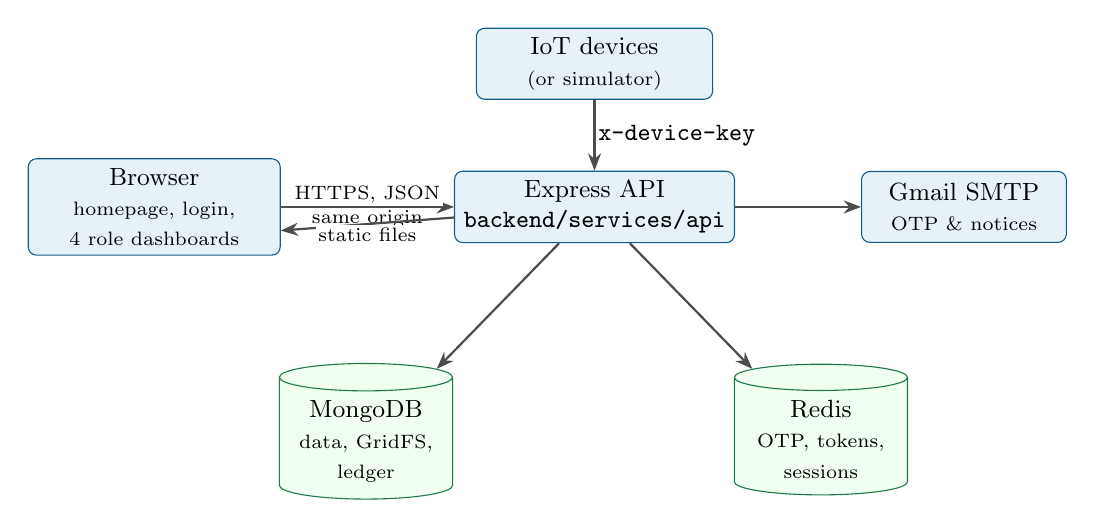
\begin{tikzpicture}[node distance=1.2cm and 1.5cm]
  \node[box,minimum width=3.2cm] (browser) {Browser\\\scriptsize homepage, login,\\\scriptsize 4 role dashboards};
  \node[box,minimum width=3.2cm,right=2.2cm of browser] (api) {Express API\\\scriptsize \code{backend\codesl{}services\codesl{}api}};
  \node[box,minimum width=3.0cm,above=0.9cm of api] (iot) {IoT devices\\\scriptsize (or simulator)};
  \node[store,below left=1.6cm and 0.2cm of api] (mongo) {MongoDB\\\scriptsize data, GridFS,\\\scriptsize ledger};
  \node[store,below right=1.6cm and 0.2cm of api] (redis) {Redis\\\scriptsize OTP, tokens,\\\scriptsize sessions};
  \node[box,minimum width=2.6cm,right=1.6cm of api] (smtp) {Gmail SMTP\\\scriptsize OTP \& notices};
  \draw[arr] (browser) -- node[lbl,above]{HTTPS, JSON} node[lbl,below]{same origin} (api);
  \draw[arr] (api) -- node[lbl,below]{static files} ([yshift=-3mm]browser.east);
  \draw[arr] (iot) -- node[lbl,right]{\code{x-device-key}} (api);
  \draw[arr] (api) -- (mongo);
  \draw[arr] (api) -- (redis);
  \draw[arr] (api) -- (smtp);
\end{tikzpicture}
\caption{System context}\label{fig:context}
\end{figure}

\begin{itemize}
  \item \textbf{Browser.} Plain HTML, CSS and JavaScript, served by the API
    itself. Being on the same origin lets the refresh-token cookie be
    \code{SameSite=Strict} and removes the need for CORS in the browser.
  \item \textbf{API.} One Node.js/Express service. It is split internally into
    modules (auth, appointments, records, \ldots) that share middleware and
    services.
  \item \textbf{MongoDB} stores all business data, uploaded files (GridFS) and
    the ledger (\code{ledgerentries} collection).
  \item \textbf{Redis} stores short-lived security state: hashed OTPs, refresh
    token ids, the access-token blacklist, cached session state and attempt
    counters. Everything in Redis expires on its own.
  \item \textbf{SMTP} (Gmail) delivers OTP codes, welcome and verification emails.
  \item \textbf{IoT devices} post readings with their own API key; they never
    hold a user session.
\end{itemize}

\section{Inside the API}

\begin{figure}[H]
\centering
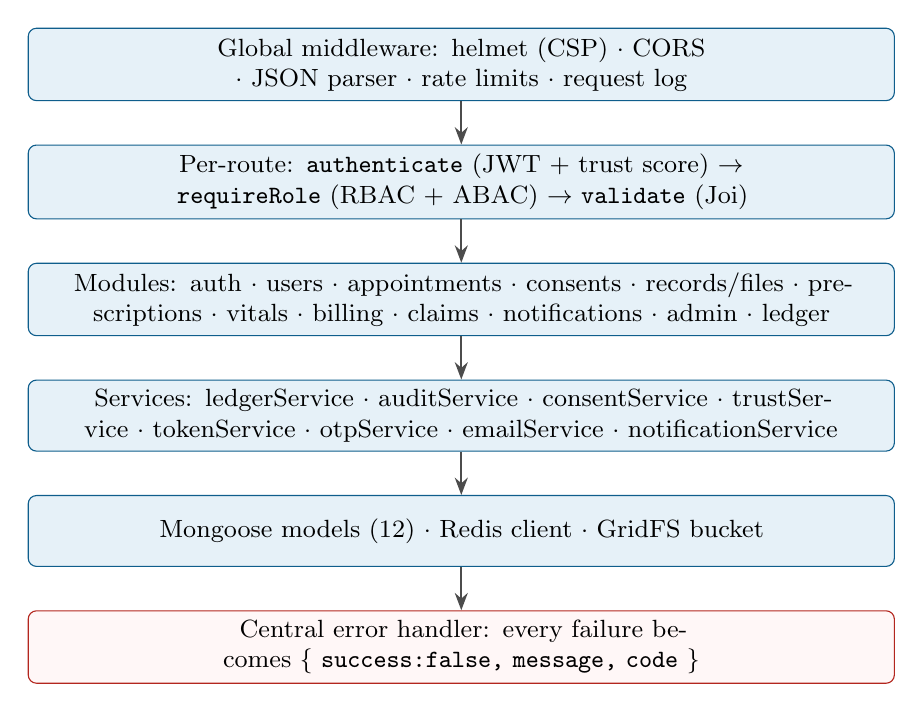
\begin{tikzpicture}[node distance=0.55cm]
  \node[box,minimum width=11cm,text width=10.6cm] (mw) {Global middleware: helmet (CSP) $\cdot$ CORS $\cdot$ JSON parser $\cdot$ rate limits $\cdot$ request log};
  \node[box,minimum width=11cm,text width=10.6cm,below=of mw] (auth) {Per-route: \code{authenticate} (JWT + trust score) $\to$ \code{requireRole} (RBAC + ABAC) $\to$ \code{validate} (Joi)};
  \node[box,minimum width=11cm,text width=10.6cm,below=of auth] (mod) {Modules: auth $\cdot$ users $\cdot$ appointments $\cdot$ consents $\cdot$ records/files $\cdot$ prescriptions $\cdot$ vitals $\cdot$ billing $\cdot$ claims $\cdot$ notifications $\cdot$ admin $\cdot$ ledger};
  \node[box,minimum width=11cm,text width=10.6cm,below=of mod] (svc) {Services: ledgerService $\cdot$ auditService $\cdot$ consentService $\cdot$ trustService $\cdot$ tokenService $\cdot$ otpService $\cdot$ emailService $\cdot$ notificationService};
  \node[box,minimum width=11cm,text width=10.6cm,below=of svc] (mdl) {Mongoose models (12) $\cdot$ Redis client $\cdot$ GridFS bucket};
  \node[box,minimum width=11cm,text width=10.6cm,below=of mdl,draw=badred,fill=red!3] (err) {Central error handler: every failure becomes \code{\{ success:false, message, code \}}};
  \foreach \a/\b in {mw/auth,auth/mod,mod/svc,svc/mdl,mdl/err} \draw[arr] (\a) -- (\b);
\end{tikzpicture}
\caption{Layers inside the API}\label{fig:layers}
\end{figure}

The rule that keeps this maintainable: \emph{route handlers do HTTP; services
do policy}. For example, every module that touches a patient's data calls the
same \code{consentService.assertCanAccessPatient}, and every module that changes
protected data calls the same \code{ledgerService.recordEvent}. There is exactly
one implementation of ``may this doctor see this patient?'' and one of ``write a
ledger entry''.

\section{Technology stack and why}

\begin{table}[H]
\centering\small
\caption{Technology choices}\label{tab:stack}
\begin{tabularx}{\textwidth}{@{}P{3cm}P{3.4cm}Y@{}}
\toprule
\textbf{Concern} & \textbf{Choice} & \textbf{Why} \\
\midrule
Runtime / framework & Node.js 18+, Express 4 & Already used by the original auth service; small and well understood. \\
Database & MongoDB + Mongoose 8 & Already in the repo. Flexible documents suit per-role profiles; unique and partial indexes give real integrity guarantees. \\
Files & GridFS & Lives in the same MongoDB, no extra service; streams large files. \\
Security state & Redis 4 client & TTL on every key: OTPs and blacklist entries clean themselves up. \\
Auth & bcryptjs, jsonwebtoken & Standard password hashing and signed tokens. \\
Validation & Joi 17 & Declarative schemas, all errors reported at once. \\
HTTP hardening & helmet, express-rate-limit, cors & CSP and security headers, brute-force limits. \\
Uploads & multer 2 & Multipart parsing with type and size limits. \\
Email & Nodemailer 6 & SMTP (Gmail) in production; console and in-memory transports for development and tests. \\
Logging & winston 3 & Console plus rotating files in \file{backend\codesl{}logs} (git-ignored). \\
Frontend & Vanilla JS, Chart.js 4.4.1, Lucide 0.460.0 & No build step; the existing pages were kept (D4). \\
Tests & Jest 29, Supertest 7, jsdom, Testing Library & Real HTTP requests against real Mongo and Redis. \\
\bottomrule
\end{tabularx}
\end{table}

\section{Architecture decisions}\label{sec:decisions}

\code{PLAN.md} \S3 locked six decisions before any feature code was written.
Their outcomes:

\begin{description}[style=nextline,leftmargin=1cm]
  \item[D1 -- One database.] MongoDB for everything; no PostgreSQL. A second
    database would add risk with no user-facing benefit at this scale.
  \item[D2 -- Hash chain instead of Hyperledger Fabric.] Fabric needs a network
    of certificate authorities, peers and an orderer, plus chaincode lifecycle
    management: a project in itself. The paper's actual requirement is
    \emph{immutable, tamper-evident and auditable}. A hash chain meets that inside
    the existing database (Chapter~\ref{ch:ledger} shows how).
  \item[D3 -- GridFS instead of IPFS.] The pattern from the paper is kept:
    the file lives in storage, its SHA-256 lives in the ledger. Only the storage
    backend differs.
  \item[D4 -- Keep the vanilla frontend.] The existing HTML/CSS was substantial,
    so it was wired to the API instead of rewritten in React. Shared state that
    Redux would have held lives in two small modules (\file{js\codesl{}api\codedot{}js},
    \file{js\codesl{}portal\codedot{}js}).
  \item[D5 -- Redis has a defined job.] OTPs, refresh tokens, revocation,
    session cache and attempt counters. Nothing else.
  \item[D6 -- Trust score is a real feature.] The \code{MIN\_TRUST\_SCORE} and
    \code{HIGH\_SENSITIVITY\_TRUST\_SCORE} settings were found to belong to a
    documented zero-trust design. They are now enforced on every request
    (Chapter~\ref{ch:zerotrust}).
\end{description}

\section{Why a hash chain is enough}

A blockchain such as Fabric solves two problems: \emph{tamper evidence} (you can
tell if history was changed) and \emph{decentralised trust} (no single party can
change history, because many independent parties hold copies). MediChain is run
by one hospital, so the second problem does not arise in the same form: there is
no group of mutually distrusting organisations. The first problem is exactly what
a hash chain solves. Section~\ref{sec:ledger-limits} discusses the remaining gap
(an attacker who can rewrite the \emph{whole} chain) and how to close it by
publishing the chain's head hash externally.

\section{Repository layout}

\begin{lstlisting}[style=shell,caption={Repository layout}]
backend/services/api/
  src/
    app.js, server.js        Express app and process start-up
    config/config.js          environment -> config object, validation
    db/                       mongo.js (connection, GridFS), redis.js
    middleware/               auth.js, validate.js, errorHandler.js
    models/                   12 Mongoose models
    services/                 ledger, audit, consent, trust, token, otp, email, notification
    modules/<area>/           route files (and helpers) per feature area
    utils/                    errors.js, hash.js, logger.js
  scripts/                    seed, IoT simulator, tamper demo, ledger verifier
  tests/                      unit/ and integration/ (Jest + Supertest)
frontend/
  homepage.html, login.html   public pages
  patient.html, doctor.html, admin.html, insurance.html
  css/portal.css              shared dashboard styles
  js/api.js, ui.js, portal.js shared client code
  js/patient.js, doctor.js, admin.js, insurance.js
  tests/                      Jest + jsdom tests
docs/                         this document, DEMO.md, zero-trust notes
Dockerfile, docker-compose.yml, .github/workflows/ci.yml
\end{lstlisting}

%% =====================================================================
\chapter{Setup and Running}\label{ch:setup}

\section{Prerequisites}

\begin{itemize}
  \item Node.js 18 or newer (developed on 24, Docker image uses 20).
  \item MongoDB 6+ and Redis 6+, either installed locally (macOS:
    \code{brew install mongodb-community redis}) or through Docker.
  \item For real OTP emails: a Gmail account with 2-step verification and an
    \emph{app password} (Google Account $\to$ Security $\to$ App passwords).
\end{itemize}

\section{Environment variables}\label{sec:env}

All configuration comes from \file{backend\codesl{}services\codesl{}api\codesl{}\codedot{}env}
(copied from \file{\codedot{}env\codedot{}example} at the repository root; the real
\file{\codedot{}env} is git-ignored).

\begin{longtable}{@{}P{4.6cm}P{2.6cm}P{6.8cm}@{}}
\caption{Environment variables}\label{tab:env}\\
\toprule
\textbf{Variable} & \textbf{Default} & \textbf{Meaning} \\
\midrule
\endfirsthead
\toprule
\textbf{Variable} & \textbf{Default} & \textbf{Meaning} \\
\midrule
\endhead
\code{PORT} & 8001 & HTTP port (API and frontend) \\
\code{NODE\_ENV} & development & \code{production} enables secure cookies, hides error details, requires SMTP \\
\code{MONGODB\_URI} & \emph{required} & e.g. \code{mongodb:\codesl{}\codesl{}127.0.0.1:27017\codesl{}medichain} \\
\code{JWT\_SECRET} & \emph{required} & Signs access tokens; \code{openssl rand -hex 64} \\
\code{JWT\_REFRESH\_SECRET} & \emph{required} & Signs refresh tokens; must differ from \code{JWT\_SECRET} \\
\code{JWT\_EXPIRY} & 15m & Access-token lifetime \\
\code{JWT\_REFRESH\_EXPIRY\_DAYS} & 7 & Refresh-token lifetime \\
\code{EMAIL\_TRANSPORT} & smtp & \code{smtp} sends mail; \code{console} prints it to the log (development only); \code{json} keeps it in memory (tests) \\
\code{EMAIL\_SERVICE} & -- & Nodemailer service name, e.g. \code{gmail} \\
\code{EMAIL\_USER}, \code{EMAIL\_PASSWORD} & \emph{required for smtp} & Gmail address and app password \\
\code{EMAIL\_FROM} & \code{EMAIL\_USER} & Sender shown in emails \\
\code{OTP\_EXPIRY\_MINUTES} & 10 & OTP lifetime \\
\code{OTP\_LENGTH} & 6 & Digits per OTP \\
\code{OTP\_MAX\_ATTEMPTS} & 10 & OTP requests + wrong codes per email per 15 minutes \\
\code{REDIS\_HOST}, \code{REDIS\_PORT}, \code{REDIS\_DB} & localhost, 6379, 0 & Redis connection \\
\code{MIN\_TRUST\_SCORE} & 50 & Trust score needed for any authenticated request \\
\code{HIGH\_SENSITIVITY\_TRUST\_SCORE} & 70 & Trust score needed for medical records and files \\
\code{MAX\_FAILED\_LOGINS} & 5 & Failures before the account locks \\
\code{ACCOUNT\_LOCK\_MINUTES} & 30 & Lock duration \\
\code{RATE\_LIMIT\_WINDOW\_MINUTES} & 15 & Rate-limit window \\
\code{RATE\_LIMIT\_MAX} & 1000 & Requests per IP per window, all of \code{\codesl{}api} \\
\code{AUTH\_RATE\_LIMIT\_MAX} & 30 & Requests per IP per window to login and register \\
\code{MAX\_UPLOAD\_MB} & 10 & Largest accepted file \\
\code{ALLOWED\_ORIGINS} & \code{http:\codesl{}\codesl{}localhost:8001} & Cross-origin callers (the bundled frontend needs none) \\
\code{SEED\_EMAIL\_BASE} & -- & Seed only: demo accounts become plus-addresses of this email \\
\code{SEED\_DEMO\_PASSWORD} & -- & Seed only: password shared by all demo accounts \\
\bottomrule
\end{longtable}

\begin{note}[Plus-addressing for the demo]
Gmail delivers \code{you+patient@gmail.com} to \code{you@gmail.com}. The seed
script creates every demo account as such an address of \code{SEED\_EMAIL\_BASE},
so one inbox receives the OTP codes of all eight demo users, yet each account
still has its own unique email.
\end{note}

\section{Running locally}

\begin{lstlisting}[style=shell,caption={First run on macOS}]
brew services start mongodb-community
brew services start redis
cp .env.example backend/services/api/.env     # then edit it (Section 4.2)
cd backend/services/api
npm install
npm run seed -- --reset                        # demo hospital
npm run dev                                    # http://localhost:8001
\end{lstlisting}

\section{Running with Docker}

\begin{lstlisting}[style=shell,caption={Docker Compose}]
docker compose up --build -d                   # mongo + redis + api
docker compose exec api node scripts/seed.js --reset
\end{lstlisting}

The compose file runs the API with \code{NODE\_ENV=production}, which requires
\code{EMAIL\_TRANSPORT=smtp}. To try it with console OTPs instead, start it with
\code{NODE\_ENV=development docker compose up --build -d}.

\section{Scripts}

\begin{table}[H]
\centering\small
\caption{npm scripts in \file{backend\codesl{}services\codesl{}api}}\label{tab:scripts}
\begin{tabularx}{\textwidth}{@{}P{5.2cm}Y@{}}
\toprule
\textbf{Command} & \textbf{Purpose} \\
\midrule
\code{npm run dev} / \code{npm start} & Start with auto-reload (nodemon) / plain node \\
\code{npm test} & All backend tests (own databases, never touches dev data) \\
\code{npm run test:coverage} & Tests with a coverage report \\
\code{npm run seed -- --reset} & Drop the database and load the demo hospital \\
\code{npm run demo:iot} & Stream device readings (\code{--interval N}, \code{--spike}) \\
\code{npm run demo:tamper} & Edit a record directly in MongoDB (\code{--ledger}, \code{--restore}) \\
\code{npm run ledger:verify} & Full integrity check from the command line \\
\bottomrule
\end{tabularx}
\end{table}

\section{The demo data}\label{sec:seed}

\file{scripts\codesl{}seed\codedot{}js} creates a small but realistic hospital
so that every screen has something to show:

\begin{itemize}
  \item hospital settings (departments, four insurers, booking window);
  \item one admin; Dr Ananya Iyer (Cardiology) and Dr Rahul Menon
    (Endocrinology), both verified; Dr Kavya Reddy (Dermatology), pending;
    agent Priya Sharma (Star Health);
  \item patients Arjun Mehta (hypertension, consent to Dr Iyer, BP monitor),
    Meera Nair (type 2 diabetes, pulse oximeter) and Rohan Gupta (no consent to
    anyone: the break-glass patient);
  \item past, today's and upcoming appointments; records with real attached
    files; prescriptions including a pending refill; bills and claims in
    several states; seven days of device readings; notifications.
\end{itemize}

The seed is a script, not application code: it writes directly to MongoDB.
But it writes every protected document through \code{ledgerService} exactly as
the API would, so ``Verify ledger'' reports a valid chain straight after
seeding.

\begin{lstlisting}[language=JavaScript,caption={How the seed derives demo emails (\file{scripts/seed.js})}]
const base = requireEnv('SEED_EMAIL_BASE');
// ...
const [local, domain] = base.split('@');
const email = (tag) => `${local}+${tag}@${domain}`;   // you+patient@gmail.com
\end{lstlisting}

%% =====================================================================
\chapter{Backend Foundation}\label{ch:foundation}

Before any feature, every request passes through the same foundation: the
configuration, the Express application with its security middleware, input
validation and the central error handler. This chapter explains each piece.

\section{Life of a request}

Take \code{GET \codesl{}api\codesl{}records?patientId=...} sent by a doctor. In order:

\begin{enumerate}
  \item \textbf{helmet} adds security headers (CSP, \code{nosniff}, \ldots).
  \item \textbf{CORS}, \textbf{cookie-parser} and the \textbf{JSON parser}
    (100\,kB limit) run.
  \item The \textbf{rate limiter} counts the request against the caller's IP.
  \item The router for \code{\codesl{}api\codesl{}records} runs \textbf{authenticate}: verify
    the JWT, check it is not revoked, load the account state, compute the
    trust score (Chapter~\ref{ch:zerotrust}).
  \item \textbf{requireRole}\code{('patient','doctor', \{minTrustScore:70, allowBreakGlass:true\})}
    checks the role, approval status and trust score.
  \item \textbf{validate} checks the query string against a Joi schema.
  \item The handler calls \textbf{consentService} (does this doctor have
    consent?) and then MongoDB.
  \item If anything throws, the \textbf{error handler} turns it into JSON.
  \item Allow and deny decisions are written to the \textbf{access chain} of
    the ledger.
\end{enumerate}

\section{Configuration: \file{src\codesl{}config\codesl{}config\codedot{}js}}

\textbf{Purpose.} Turn environment variables into one typed object, and refuse
to start if the configuration is missing or unsafe.

\textbf{Why.} The original service started with missing secrets and failed
later on the first login, with an obscure error. Failing at start-up is cheaper
to debug and can never half-work in production.

\begin{lstlisting}[language=JavaScript,caption={Start-up validation (\file{src/config/config.js})}]
function validateConfig(cfg = config, rawEnv = env) {
  const required = ['MONGODB_URI', 'JWT_SECRET', 'JWT_REFRESH_SECRET'];
  if (cfg.email.transport === 'smtp') {
    required.push('EMAIL_USER', 'EMAIL_PASSWORD');
  }

  const missing = required.filter((key) => !rawEnv[key] || String(rawEnv[key]).trim() === '');
  if (missing.length > 0) {
    throw new Error(`Missing required environment variables: ${missing.join(', ')}`);
  }

  if (!['smtp', 'console', 'json'].includes(cfg.email.transport)) {
    throw new Error(`EMAIL_TRANSPORT must be smtp, console or json (got "${cfg.email.transport}")`);
  }

  // Printing OTPs to a log is only acceptable on a developer machine.
  if (cfg.isProduction && cfg.email.transport !== 'smtp') {
    throw new Error('EMAIL_TRANSPORT must be "smtp" in production');
  }

  if (rawEnv.JWT_SECRET === rawEnv.JWT_REFRESH_SECRET) {
    throw new Error('JWT_SECRET and JWT_REFRESH_SECRET must be different');
  }

  return true;
}
\end{lstlisting}

\begin{howto}
\begin{itemize}
  \item Email credentials are required only when mail is really sent
    (\code{smtp}).
  \item The \code{console} transport prints OTP codes to the log, which is
    convenient on a laptop and a security hole on a server, so production
    rejects it.
  \item If both JWT secrets were equal, a refresh token could be presented as an
    access token. Requiring different secrets closes that.
  \item The function takes \code{cfg} and \code{rawEnv} as parameters so unit
    tests can call it with fake environments.
\end{itemize}
\end{howto}

\section{Process start-up: \file{src\codesl{}server\codedot{}js}}

\begin{lstlisting}[language=JavaScript,caption={Start-up order (\file{src/server.js})}]
async function start() {
  try {
    config.validateConfig();
    await connectMongo();
    await connectRedis();
    await HospitalSettings.getSingleton();
    await emailService.verifyConnection();

    const app = require('./app');
    const server = app.listen(config.port, () => {
      logger.info(`MediChain API listening on http://localhost:${config.port} (${config.nodeEnv})`);
    });

    const shutdown = (signal) => {
      logger.info(`${signal} received, shutting down`);
      server.close(async () => {
        await Promise.allSettled([disconnectMongo(), disconnectRedis()]);
        process.exit(0);
      });
      setTimeout(() => process.exit(1), 10000).unref();
    };
    process.on('SIGTERM', () => shutdown('SIGTERM'));
    process.on('SIGINT', () => shutdown('SIGINT'));
  } catch (error) {
    logger.error(`Failed to start: ${error.message}`);
    process.exit(1);
  }
}
\end{lstlisting}

\begin{howto}
The server listens only after every dependency answered. \code{connectRedis}
sends a \code{PING} and throws if Redis is not there (the old service swallowed
this error and then failed every login). \code{HospitalSettings.getSingleton()}
creates the settings document on first run. \code{verifyConnection} logs into
SMTP so a wrong Gmail app password shows up in the log at start-up, not at the
first login. On \code{SIGTERM} (Docker stop) the server stops accepting
connections, finishes in-flight requests and closes the databases; if that takes
longer than 10\,s it exits anyway.
\end{howto}

\section{The Express application: \file{src\codesl{}app\codedot{}js}}

\subsection{Security headers and the Content-Security-Policy}

\begin{lstlisting}[language=JavaScript,caption={helmet and CSP (\file{src/app.js})}]
// The frontend is served by this same server, so a strict Content-Security-Policy
// can allow scripts only from this origin plus two pinned CDNs. Inline <script>
// and onclick="" handlers are blocked, which shuts the main door to XSS.
app.use(helmet({
  contentSecurityPolicy: {
    useDefaults: true,
    directives: {
      'script-src': ["'self'", 'https://cdn.jsdelivr.net', 'https://unpkg.com'],
      'style-src': ["'self'", "'unsafe-inline'", 'https://fonts.googleapis.com', 'https://cdn.jsdelivr.net'],
      'font-src': ["'self'", 'https://fonts.gstatic.com', 'data:'],
      'img-src': ["'self'", 'data:', 'blob:', 'https://images.pexels.com'],
      'connect-src': ["'self'"],
      'frame-src': ["'self'", 'blob:'],
      'object-src': ["'self'", 'blob:'],
      'upgrade-insecure-requests': config.isProduction ? [] : null,
    },
  },
  crossOriginEmbedderPolicy: false,
}));
\end{lstlisting}

\begin{howto}
A Content-Security-Policy tells the browser which sources it may load code from.
With \code{script-src 'self'} and no \code{'unsafe-inline'}, even if an attacker
manages to get \code{<script>alert(1)<\codesl{}script>} into a patient's name, the browser
refuses to run it. This is why the frontend has no inline scripts and no
\code{onclick=} attributes: all handlers are attached from \code{.js} files.
\code{connect-src 'self'} means page scripts can only call this API. \code{blob:}
in \code{frame-src}/\code{object-src} lets the dashboards preview downloaded PDFs.
\end{howto}

\subsection{Rate limits}

\begin{lstlisting}[language=JavaScript,caption={Two rate limiters (\file{src/app.js})}]
app.use('/api/', rateLimit({
  windowMs, max: config.rateLimit.max, standardHeaders: true, legacyHeaders: false,
  message: limiterResponse('Too many requests from this IP, please try again later.'),
  skip: () => config.isTest,
}));

// Stricter budget for the endpoints an attacker would hammer to guess passwords or codes.
const authLimiter = rateLimit({
  windowMs, max: config.rateLimit.authMax, standardHeaders: true, legacyHeaders: false,
  message: limiterResponse('Too many login attempts from this IP. Try again in 15 minutes.'),
  skip: () => config.isTest,
});
app.use(['/api/auth/login', '/api/auth/register'], authLimiter);
\end{lstlisting}

The general limit protects the whole API; the second, much smaller budget
(30 per 15 minutes by default) applies to login and registration, the endpoints
used for password and OTP guessing. Per-account limits (lockout, OTP attempts)
are added on top in Chapter~\ref{ch:auth}, so an attacker spreading requests
over many IPs still hits a wall.

\subsection{Routes and the bundled frontend}

\begin{lstlisting}[language=JavaScript,caption={Module mounting and static frontend (\file{src/app.js})}]
app.use('/api/auth', require('./modules/auth/auth.routes'));
app.use('/api', require('./modules/users/users.routes'));
app.use('/api/appointments', require('./modules/appointments/appointments.routes'));
app.use('/api/consents', require('./modules/consents/consents.routes'));
app.use('/api/records', require('./modules/records/records.routes'));
app.use('/api/files', require('./modules/records/files.routes'));
app.use('/api/prescriptions', require('./modules/prescriptions/prescriptions.routes'));
app.use('/api', require('./modules/vitals/vitals.routes'));
app.use('/api/bills', require('./modules/billing/billing.routes'));
app.use('/api/claims', require('./modules/claims/claims.routes'));
app.use('/api/notifications', require('./modules/notifications/notifications.routes'));
app.use('/api/admin', require('./modules/admin/admin.routes'));
app.use('/api/ledger', require('./modules/ledger/ledger.routes'));
app.use('/api', notFoundHandler);

// Same origin as the API: the SameSite=Strict refresh cookie just works and no
// CORS is needed in the browser. Development files are never served.
app.use((req, res, next) => (/^\/(node_modules|tests|package(-lock)?\.json|jest\.config)/.test(req.path) ? notFoundHandler(req, res) : next()));
app.use(express.static(config.frontendDir, { index: 'homepage.html', extensions: ['html'] }));
\end{lstlisting}

The \code{\codesl{}api} 404 handler is mounted \emph{before} the static files, so a
mistyped API path returns a JSON 404 instead of an HTML page. The regular
expression blocks the frontend's development files (its \code{node\_modules},
tests and \code{package.json}) from being served.

\section{Errors: \file{src\codesl{}utils\codesl{}errors\codedot{}js} and the error handler}

\begin{lstlisting}[language=JavaScript,caption={AppError and asyncHandler (\file{src/utils/errors.js})}]
class AppError extends Error {
  constructor(status, message, code, details) {
    super(message);
    this.name = 'AppError';
    this.status = status;
    this.code = code || undefined;
    this.details = details || undefined;
  }
}

const badRequest = (message, details) => new AppError(400, message, 'BAD_REQUEST', details);
const unauthorized = (message, code = 'UNAUTHORIZED') => new AppError(401, message, code);
const forbidden = (message, code = 'FORBIDDEN') => new AppError(403, message, code);
const notFound = (message = 'Resource not found') => new AppError(404, message, 'NOT_FOUND');
const conflict = (message, code = 'CONFLICT') => new AppError(409, message, code);
// ...
const asyncHandler = (fn) => (req, res, next) => Promise.resolve(fn(req, res, next)).catch(next);
\end{lstlisting}

\begin{howto}
Handlers simply \code{throw conflict('This slot has just been booked...', 'SLOT\_TAKEN')}.
Express 4 does not catch errors thrown from \code{async} functions, so every
handler is wrapped in \code{asyncHandler}, which forwards a rejected promise to
\code{next(error)}. The central handler then produces the response. The
machine-readable \code{code} lets the frontend react to specific errors (for
example \code{SESSION\_ENDED} sends the user back to the login page).
\end{howto}

\begin{lstlisting}[language=JavaScript,caption={Central error handler, mapping section (\file{src/middleware/errorHandler.js})}]
  if (err.message === 'REDIS_UNAVAILABLE') {
    status = 503;
    message = 'Security service temporarily unavailable. Please try again.';
    code = 'SERVICE_UNAVAILABLE';
  } else if (err instanceof multer.MulterError) {
    status = err.code === 'LIMIT_FILE_SIZE' ? 413 : 400;
    message = err.code === 'LIMIT_FILE_SIZE' ? 'File is too large' : err.message;
    code = err.code;
  } else if (err.name === 'ValidationError') {
    status = 400;
    message = Object.values(err.errors).map((e) => e.message).join(', ');
  } else if (err.name === 'CastError') {
    status = 400;
    message = `Invalid ${err.path}`;
  } else if (err.code === 11000) {
    status = 409;
    message = 'A record with these details already exists';
    code = 'DUPLICATE';
  } else if (err.type === 'entity.too.large') {
    status = 413;
    message = 'Request body is too large';
  } else if (err.type === 'entity.parse.failed') {
    status = 400;
    message = 'Malformed JSON body';
  }

  if (status >= 500) {
    logger.error(`${req.method} ${req.originalUrl} -> ${err.stack || err.message}`);
    if (config.isProduction) message = 'Internal server error';
  }
\end{lstlisting}

Each branch converts a low-level failure into a meaningful HTTP status. The most
important one is the first: when Redis is down, the security layer cannot check
OTPs, refresh tokens or revocations, so the request fails with \textbf{503}
(``fail closed'') rather than being let through. In production, details of
unexpected (500) errors are logged but not sent to the client.

\section{Input validation: \file{src\codesl{}middleware\codesl{}validate\codedot{}js}}

\begin{lstlisting}[language=JavaScript,caption={The validate middleware (\file{src/middleware/validate.js})}]
const validate = (schemas) => (req, res, next) => {
  const errors = [];
  for (const part of ['params', 'query', 'body']) {
    if (!schemas[part]) continue;
    const { error, value } = schemas[part].validate(req[part] || {}, {
      abortEarly: false, stripUnknown: false, convert: true,
    });
    if (error) {
      errors.push(...error.details.map((d) => d.message.replace(/"/g, '')));
    } else if (part === 'query') {
      Object.defineProperty(req, 'query', { value, writable: true, configurable: true });
    } else {
      req[part] = value;
    }
  }
  if (errors.length) {
    return res.status(400).json({ success: false, message: 'Validation failed', errors });
  }
  return next();
};

const objectId = () => Joi.string().pattern(/^[a-f\d]{24}$/i).message('must be a valid id');

const password = () => Joi.string()
  .min(8)
  .max(128)
  .pattern(/^(?=.*[a-z])(?=.*[A-Z])(?=.*\d)(?=.*[@$!%*?&#^()\-_=+]).+$/)
\end{lstlisting}

\begin{howto}
Each route declares what it accepts, for example
\code{validate(\{ body: Joi.object(\{ doctorId: objectId().required(), ... \}) \})}.
\begin{itemize}
  \item \code{abortEarly:false} reports \emph{every} problem at once, so a form
    can show all errors together.
  \item \code{stripUnknown:false} means unknown fields are an error, not silently
    dropped: a client cannot sneak in \code{role:'admin'}.
  \item \code{convert:true} turns \code{"7"} into \code{7} and ISO strings into
    dates; the cleaned value replaces the original, so handlers work with
    trusted, typed data. (\code{req.query} is a getter in newer Express, hence
    \code{defineProperty}.)
\end{itemize}
\end{howto}

\section{Databases: \file{src\codesl{}db\codesl{}}}

\begin{lstlisting}[language=JavaScript,caption={GridFS bucket (\file{src/db/mongo.js})}]
/**
 * GridFS stores files larger than a normal document by splitting them into
 * 255 kB chunks (collections `uploads.files` and `uploads.chunks`). It ships
 * with the MongoDB driver, so no extra infrastructure is needed (decision D3).
 */
function getBucket() {
  if (!bucket) {
    bucket = new mongoose.mongo.GridFSBucket(mongoose.connection.db, { bucketName: 'uploads' });
  }
  return bucket;
}
\end{lstlisting}

\begin{lstlisting}[language=JavaScript,caption={Redis connection that fails loudly (\file{src/db/redis.js})}]
async function connectRedis() {
  if (!redisClient.isOpen) {
    await redisClient.connect();
  }
  await redisClient.ping();
  return redisClient;
}
\end{lstlisting}

\section{Hashing helpers: \file{src\codesl{}utils\codesl{}hash\codedot{}js}}

These three functions underpin the ledger (Chapter~\ref{ch:ledger}).

\begin{lstlisting}[language=JavaScript,caption={Canonical JSON and hashing (\file{src/utils/hash.js})}]
const sha256 = (value) => crypto.createHash('sha256').update(typeof value === 'string' || Buffer.isBuffer(value) ? value : String(value ?? '')).digest('hex');

/**
 * Deterministic JSON: object keys are sorted at every level, so the same data
 * always produces the same string (and therefore the same hash) no matter in
 * which order the fields were assigned.
 */
function canonicalJSON(value) {
  if (value === null || value === undefined) return 'null';
  if (value instanceof Date) return JSON.stringify(value.toISOString());
  if (Array.isArray(value)) return `[${value.map(canonicalJSON).join(',')}]`;
  if (typeof value === 'object') {
    if (typeof value.toHexString === 'function') return JSON.stringify(value.toHexString()); // ObjectId
    const keys = Object.keys(value).filter((k) => value[k] !== undefined).sort();
    return `{${keys.map((k) => `${JSON.stringify(k)}:${canonicalJSON(value[k])}`).join(',')}}`;
  }
  return JSON.stringify(value);
}

const hashObject = (value) => sha256(canonicalJSON(value));
\end{lstlisting}

\begin{howto}[Why canonical JSON matters]
\code{JSON.stringify(\{a:1,b:2\})} and \code{JSON.stringify(\{b:2,a:1\})} produce
different strings, and therefore different hashes, for the same data. MongoDB
does not promise to return fields in the order they were written. Sorting the
keys at every level, and writing dates and ObjectIds in one fixed format, makes
the hash a function of the \emph{data} only. Without this, verification would
report false tampering.
\end{howto}

%% =====================================================================
\chapter{Authentication and Sessions}\label{ch:auth}

This chapter covers who a user is (the \code{User} model), how they prove it
(password plus emailed OTP), and how the proof is carried between requests
(access and refresh tokens).

\section{The User model: \file{src\codesl{}models\codesl{}User\codedot{}js}}

One collection holds all four roles. Fields that only make sense for one role
live in a sub-document (\code{patientProfile}, \code{doctorProfile},
\code{agentProfile}).

\begin{lstlisting}[language=JavaScript,caption={User schema, key fields (\file{src/models/User.js})}]
const ROLES = ['patient', 'doctor', 'admin', 'insurance_agent'];
// Doctors and insurance agents must be approved by an admin before they can
// touch clinical or financial data. Patients and admins are approved on creation.
const ROLES_NEEDING_APPROVAL = ['doctor', 'insurance_agent'];

const userSchema = new mongoose.Schema({
  email: { type: String, required: true, unique: true, lowercase: true, trim: true },
  fullName: { type: String, trim: true, required: true },
  passwordHash: { type: String, required: true },
  role: { type: String, enum: ROLES, required: true, default: 'patient' },
  // ... phone, dateOfBirth, gender, address, patientProfile, doctorProfile, agentProfile
  approvalStatus: { type: String, enum: ['pending', 'approved', 'rejected'], default: 'approved' },
  approvalNote: { type: String, default: '' },

  // Identity of this user inside the hash-chain ledger (was `walletAddress`).
  ledgerAddress: { type: String, index: true },

  isVerified: { type: Boolean, default: false }, // proven control of the email (first OTP login)
  isActive: { type: Boolean, default: true },
  lastLogin: { type: Date, default: null },
  failedLoginAttempts: { type: Number, default: 0 },
  accountLockedUntil: { type: Date, default: null },
  refreshTokens: {
    type: [String],
    default: [],
    validate: { validator: (tokens) => tokens.length <= 5, message: 'A user can have at most 5 refresh tokens' },
  },
}, { timestamps: true });
\end{lstlisting}

A doctor's \code{doctorProfile} also holds \code{availability}: working days
(0 = Sunday), start and end hour, and slot length. Appointments are generated
from it (Chapter~\ref{ch:appointments}).

\begin{lstlisting}[language=JavaScript,caption={Password hashing and ledger address (\file{src/models/User.js})}]
userSchema.pre('save', async function hashPasswordAndAssignLedgerAddress(next) {
  try {
    if (!this.ledgerAddress) {
      this.ledgerAddress = `mc_${sha256(this._id.toString()).slice(0, 40)}`;
    }
    if (this.isModified('passwordHash')) {
      const salt = await bcrypt.genSalt(10);
      this.passwordHash = await bcrypt.hash(this.passwordHash, salt);
    }
    next();
  } catch (error) {
    next(error);
  }
});
\end{lstlisting}

\begin{howto}
Code that creates or changes a user puts the \emph{plain} password into
\code{passwordHash}; this hook replaces it with a bcrypt hash before anything is
written. \code{isModified} ensures an already-hashed password is not hashed
again on an unrelated save. bcrypt is deliberately slow (cost 10, about 2\textsuperscript{10}
rounds), so a stolen database cannot be brute-forced quickly. The
\code{ledgerAddress} is a stable pseudonymous identifier derived from the user
id, the successor of the paper's blockchain wallet address.
\end{howto}

\begin{lstlisting}[language=JavaScript,caption={Never leaking secrets in JSON (\file{src/models/User.js})}]
userSchema.methods.toJSON = function toJSON() {
  const obj = this.toObject();
  delete obj.passwordHash;
  delete obj.failedLoginAttempts;
  delete obj.accountLockedUntil;
  delete obj.refreshTokens;
  delete obj.__v;
  // Hide the other roles' (empty) profile sections. When a partial populate did
  // not select `role`, keep whatever profile fields were explicitly selected.
  if (obj.role) {
    if (obj.role !== 'patient') delete obj.patientProfile;
    if (obj.role !== 'doctor') delete obj.doctorProfile;
    if (obj.role !== 'insurance_agent') delete obj.agentProfile;
  }
  return obj;
};
\end{lstlisting}

Express calls \code{toJSON} whenever a user is sent with \code{res.json}, so no
route can accidentally return a password hash. The \code{if (obj.role)} guard
fixes a real bug found during testing: when an appointment populated only
\code{doctorProfile.specialization} (without \code{role}), the doctor's profile
was stripped and the patient dashboard crashed.

\section{Registration}

\begin{lstlisting}[language=JavaScript,caption={register, core (\file{src/modules/auth/auth.controller.js})}]
async function register(req, res) {
  const { email, password, fullName, role, phone, dateOfBirth, gender, address } = req.body;

  if (await User.exists({ email })) {
    throw conflict('An account with this email already exists', 'EMAIL_TAKEN');
  }

  const needsApproval = User.ROLES_NEEDING_APPROVAL.includes(role);
  const user = new User({
    email,
    fullName,
    passwordHash: password, // hashed by the pre-save hook
    role,
    // ...
    approvalStatus: needsApproval ? 'pending' : 'approved',
  });
  // ... role-specific profile fields
  await user.save();
  await ledgerService.append({
    chain: 'records', entityType: 'user', entityId: user._id, action: 'REGISTER',
    actorId: user._id, actorRole: role, payload: { email: user.email, role, ledgerAddress: user.ledgerAddress },
  });

  if (needsApproval) {
    await notificationService.notifyRole('admin', {
      type: 'warning',
      title: 'New account awaiting verification',
      // ...
      page: 'verification',
    });
  }

  emailService.sendWelcome(email, fullName, role, needsApproval); // fire-and-forget by design
\end{lstlisting}

\begin{howto}
The Joi schema on the route only allows \code{role} to be \code{patient},
\code{doctor} or \code{insurance\_agent}; nobody can register as an admin. Doctors
must supply a specialization and licence number, agents a company. A doctor or
agent account starts \code{pending}: they can log in and edit their profile, but
every clinical or claims endpoint answers 403 \code{APPROVAL\_PENDING} until an
admin approves them (Section~\ref{sec:policy}). The welcome email is not awaited:
if the mail server is slow or down, registration still succeeds.
\end{howto}

\section{Two-step login}

\begin{figure}[H]
\centering
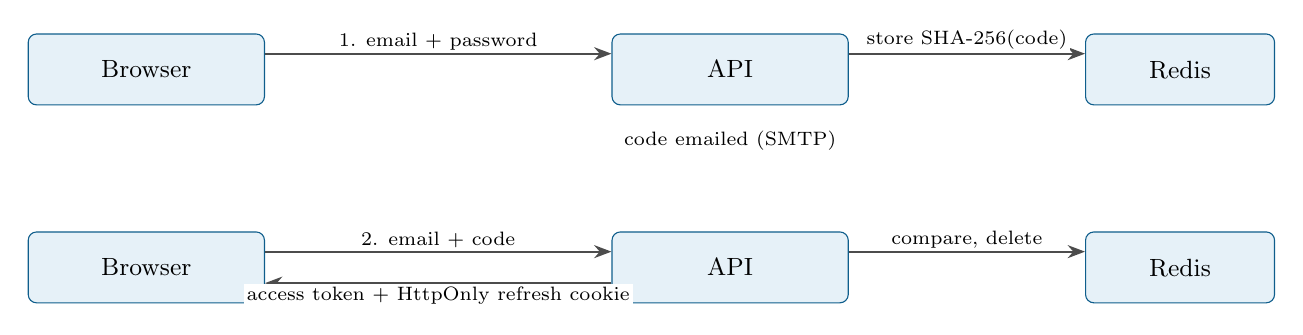
\begin{tikzpicture}[node distance=0.5cm]
  \node[box,minimum width=3cm] (b1) {Browser};
  \node[box,minimum width=3cm,right=4.4cm of b1] (a1) {API};
  \node[box,minimum width=2.4cm,right=3cm of a1] (r1) {Redis};
  \draw[arr] ([yshift=2mm]b1.east) -- node[lbl,above]{1. email + password} ([yshift=2mm]a1.west);
  \draw[arr] ([yshift=2mm]a1.east) -- node[lbl,above]{store SHA-256(code)} ([yshift=2mm]r1.west);
  \node[below=0.2cm of a1,font=\scriptsize] (mail) {code emailed (SMTP)};
  \node[box,minimum width=3cm,below=1.6cm of b1] (b2) {Browser};
  \node[box,minimum width=3cm,right=4.4cm of b2] (a2) {API};
  \node[box,minimum width=2.4cm,right=3cm of a2] (r2) {Redis};
  \draw[arr] ([yshift=2mm]b2.east) -- node[lbl,above]{2. email + code} ([yshift=2mm]a2.west);
  \draw[arr] ([yshift=2mm]a2.east) -- node[lbl,above]{compare, delete} ([yshift=2mm]r2.west);
  \draw[arr] ([yshift=-2mm]a2.west) -- node[lbl,below]{access token + HttpOnly refresh cookie} ([yshift=-2mm]b2.east);
\end{tikzpicture}
\caption{Password, then one-time code}\label{fig:login}
\end{figure}

\subsection{Step 1: \code{POST \codesl{}api\codesl{}auth\codesl{}login\codesl{}request-otp}}

\begin{lstlisting}[language=JavaScript,caption={requestOtp (\file{src/modules/auth/auth.controller.js})}]
async function requestOtp(req, res) {
  const { email, password } = req.body;
  const user = await User.findOne({ email });

  if (!user) throw unauthorized(INVALID_CREDENTIALS, 'INVALID_CREDENTIALS');
  if (user.isAccountLocked()) {
    throw forbidden('Account is locked after too many failed attempts. Try again later.', 'ACCOUNT_LOCKED');
  }
  if (!user.isActive) throw forbidden('Account is deactivated. Contact the hospital administrator.', 'ACCOUNT_DEACTIVATED');

  if (!(await user.comparePassword(password))) {
    const failed = await recordFailedAttempt(user);
    return res.status(401).json({
      success: false,
      message: INVALID_CREDENTIALS,
      code: 'INVALID_CREDENTIALS',
      attemptsRemaining: Math.max(0, config.security.maxFailedLogins - failed),
    });
  }

  if (await otpService.getAttempts(email) >= config.otp.maxAttempts) {
    throw tooMany('Too many OTP requests. Try again in 15 minutes.');
  }

  const otp = otpService.generateOTP();
  await otpService.storeOTP(email, otp);
  await emailService.sendOTP(email, otp, user.fullName);
  await otpService.incrementAttempts(email);

  res.json({
    success: true,
    message: 'A login code was sent to your email',
    data: { email, expiresInMinutes: config.otp.expiryMinutes },
  });
}
\end{lstlisting}

\begin{howto}
\begin{enumerate}
  \item An unknown email and a wrong password give the same message
    (\code{INVALID\_CREDENTIALS}), so the form cannot be used to find out who
    has an account.
  \item A wrong password increments \code{failedLoginAttempts}; at
    \code{MAX\_FAILED\_LOGINS} (5) the account is locked for 30 minutes.
  \item A per-email counter in Redis limits how many codes can be requested.
  \item \code{sendOTP} is awaited and \emph{throws} on failure: if the email
    could not be sent the user is told (500), instead of waiting for a code that
    will never arrive. (A test checks exactly this.)
\end{enumerate}
\end{howto}

\begin{lstlisting}[language=JavaScript,caption={Lockout bookkeeping (\file{src/modules/auth/auth.controller.js})}]
async function recordFailedAttempt(user) {
  const updated = await User.findByIdAndUpdate(user._id, { $inc: { failedLoginAttempts: 1 } }, { new: true });
  if (updated.failedLoginAttempts >= config.security.maxFailedLogins) {
    updated.accountLockedUntil = new Date(Date.now() + config.security.lockMinutes * 60 * 1000);
    await updated.save({ validateBeforeSave: false });
    logger.warn(`Account locked after ${updated.failedLoginAttempts} failed attempts: ${user.email}`);
  }
  await invalidateSession(user._id); // trust score reflects the failure immediately
  return updated.failedLoginAttempts;
}
\end{lstlisting}

\code{\$inc} is atomic in MongoDB, so two simultaneous wrong guesses are both
counted. Recent failures also lower the trust score of any session still open
for that user (Section~\ref{sec:trust}).

\subsection{The OTP service: \file{src\codesl{}services\codesl{}otpService\codedot{}js}}

\begin{lstlisting}[language=JavaScript,caption={Generating, storing and checking codes (\file{src/services/otpService.js})}]
  /** Only the hash is stored: a Redis dump cannot be used to log in. */
  hashOTP(otp) {
    return crypto.createHash('sha256').update(String(otp)).digest('hex');
  }

  /** Cryptographically secure, uniformly random code with no leading zero. */
  generateOTP(length = config.otp.length) {
    return crypto.randomInt(10 ** (length - 1), 10 ** length).toString();
  }

  /** Stores the hashed code with a TTL; a new request overwrites the old code. */
  storeOTP(email, otp) {
    return guard('store', () => redisClient.setEx(otpKey(email), config.otp.expiryMinutes * 60, this.hashOTP(otp)));
  }

  /** Single use: a matching code is deleted immediately. */
  verifyOTP(email, otp) {
    return guard('verify', async () => {
      const stored = await redisClient.get(otpKey(email));
      if (!stored) return { success: false, message: 'OTP expired or not found' };

      const expected = Buffer.from(stored, 'hex');
      const actual = Buffer.from(this.hashOTP(otp), 'hex');
      // Constant-time comparison: response time does not leak how many characters matched.
      if (expected.length !== actual.length || !crypto.timingSafeEqual(expected, actual)) {
        return { success: false, message: 'Invalid OTP' };
      }
      await redisClient.del(otpKey(email));
      return { success: true, message: 'OTP verified successfully' };
    });
  }
\end{lstlisting}

\begin{howto}
\begin{itemize}
  \item \code{crypto.randomInt} is a cryptographically secure generator;
    \code{Math.random} is predictable and must never be used for codes.
  \item \code{setEx} stores the code with a time-to-live: Redis deletes it after
    10 minutes without any clean-up job.
  \item Only the SHA-256 of the code is stored, like a password.
  \item \code{timingSafeEqual} always takes the same time, so an attacker cannot
    learn from response timing how close a guess was.
  \item \code{guard} converts any Redis error into \code{REDIS\_UNAVAILABLE},
    which becomes a 503: if the OTP store is down, nobody logs in.
\end{itemize}
\end{howto}

\subsection{Step 2: \code{POST \codesl{}api\codesl{}auth\codesl{}login\codesl{}verify-otp}}

\begin{lstlisting}[language=JavaScript,caption={verifyOtp, success path (\file{src/modules/auth/auth.controller.js})}]
  const result = await otpService.verifyOTP(email, otp);
  if (!result.success) {
    const otpAttempts = await otpService.incrementAttempts(email);
    const failed = await recordFailedAttempt(user);
    return res.status(401).json({ /* ... INVALID_OTP, attemptsRemaining */ });
  }

  await otpService.clearAttempts(email);
  user.failedLoginAttempts = 0;
  user.accountLockedUntil = null;
  user.lastLogin = new Date();
  user.isVerified = true;
  await user.save({ validateBeforeSave: false });
  await invalidateSession(user._id);

  const access = await issueSession(res, user);
\end{lstlisting}

A correct code resets the failure counters and marks the account
\code{isVerified} (the user has proven they control the email address, which
raises their trust score). \code{issueSession} creates the token pair.

\section{Tokens: \file{src\codesl{}services\codesl{}tokenService\codedot{}js}}

MediChain uses two tokens with different jobs:

\begin{table}[H]
\centering\small
\caption{The two tokens}\label{tab:tokens}
\begin{tabularx}{\textwidth}{@{}P{2.6cm}YY@{}}
\toprule
 & \textbf{Access token} & \textbf{Refresh token} \\
\midrule
Purpose & Sent with every API call & Gets a new access token \\
Lifetime & 15 minutes & 7 days \\
Where the browser keeps it & A JavaScript variable (memory only) & HttpOnly cookie, path \code{\codesl{}api\codesl{}auth} \\
Signed with & \code{JWT\_SECRET} & \code{JWT\_REFRESH\_SECRET} \\
Revocation & Blacklist of its \code{jti} in Redis & Valid only while its Redis key exists \\
\bottomrule
\end{tabularx}
\end{table}

\begin{lstlisting}[language=JavaScript,caption={Issuing tokens (\file{src/services/tokenService.js})}]
  /** Short-lived access token. The random jti lets us revoke this exact token. */
  generateAccessToken(user) {
    const jti = crypto.randomUUID();
    const token = jwt.sign(
      { userId: user._id.toString(), email: user.email, role: user.role, jti },
      this.config.jwt.secret,
      { expiresIn: this.config.jwt.expiry }
    );
    return { token, jti, expiresIn: this.config.jwt.expiry };
  }

  /**
   * Long-lived refresh token, signed with a different secret. It is valid only
   * while its Redis key exists, so the server can revoke it at any time.
   */
  async generateRefreshToken(user) {
    const userId = user._id.toString();
    const jti = crypto.randomUUID();
    const token = jwt.sign(
      { userId, jti, type: 'refresh' },
      this.config.jwt.refreshSecret,
      { expiresIn: `${this.config.jwt.refreshExpiryDays}d` }
    );
    try {
      await this.redis.setEx(this.refreshKey(userId, jti), this.refreshTTLSeconds, '1');
    } catch (error) {
      logger.error(`Error storing refresh token: ${error.message}`);
      throw new Error(REDIS_UNAVAILABLE);
    }
    return { token, jti, jtiHash: this.hashJTI(jti) };
  }
\end{lstlisting}

\begin{lstlisting}[language=JavaScript,caption={The refresh cookie (\file{src/modules/auth/auth.controller.js})}]
const cookieOptions = () => ({
  httpOnly: true, // JavaScript in the page cannot read it (XSS)
  secure: config.isProduction, // HTTPS-only in production; plain http://localhost works in dev
  sameSite: 'strict', // never sent on cross-site requests (CSRF)
  path: '/api/auth', // only sent to the auth endpoints that need it
  maxAge: config.jwt.refreshExpiryDays * 24 * 60 * 60 * 1000,
});
\end{lstlisting}

\begin{good}[Why the token is not in localStorage]
Anything in \code{localStorage} can be read by any script on the page; one XSS
bug would leak every user's long-lived session. Here the long-lived token is in
an \code{HttpOnly} cookie that scripts cannot read, and the short-lived access
token exists only in a variable that disappears when the tab closes. A page
reload restores the session by calling \code{\codesl{}api\codesl{}auth\codesl{}refresh-token}, which the
browser authenticates with the cookie automatically.
\end{good}

\section{Refresh-token rotation}

\begin{lstlisting}[language=JavaScript,caption={refreshToken (\file{src/modules/auth/auth.controller.js})}]
async function refreshToken(req, res) {
  const presented = req.cookies?.[REFRESH_COOKIE];
  if (!presented) throw unauthorized('No session. Please log in.', 'NO_REFRESH_TOKEN');

  let decoded;
  try {
    decoded = await tokenService.verifyRefreshToken(presented);
  } catch (error) {
    if (error.message === 'REDIS_UNAVAILABLE') throw error;
    res.clearCookie(REFRESH_COOKIE, { ...cookieOptions(), maxAge: undefined });
    throw unauthorized('Session expired. Please log in again.', 'INVALID_REFRESH_TOKEN');
  }

  const user = await User.findById(decoded.userId);
  if (!user || !user.isActive) {
    await tokenService.revokeRefreshToken(decoded.userId, decoded.jti);
    throw unauthorized('Account deactivated', 'ACCOUNT_DEACTIVATED');
  }

  await tokenService.revokeRefreshToken(decoded.userId, decoded.jti);
  await User.updateOne({ _id: user._id }, { $pull: { refreshTokens: tokenService.hashJTI(decoded.jti) } });
  const access = await issueSession(res, user);
  // ... respond with the new access token and user
}
\end{lstlisting}

\begin{howto}
Each refresh token works \emph{once}. Using it deletes its Redis key and issues
a new one in a new cookie. If an attacker steals a refresh token and uses it,
the real user's next refresh fails (its token is gone), so the theft becomes
visible. If the real user refreshes first, the stolen copy is already dead.
\code{verifyRefreshToken} also checks \code{type === 'refresh'}, so an access
token cannot be replayed here.
\end{howto}

\section{Logout, password change and deactivation}

\begin{lstlisting}[language=JavaScript,caption={Revocation on logout (\file{src/modules/auth/auth.controller.js}) and blacklisting (\file{tokenService.js})}]
async function logout(req, res) {
  await tokenService.blacklistAccessToken(req.user);
  // ... verify and revoke the refresh cookie, clear it
}

  /** Blacklists an access token until it would have expired anyway. */
  async blacklistAccessToken(decodedPayload) {
    if (!decodedPayload?.jti || !decodedPayload?.exp) throw new Error('INVALID_TOKEN');
    const ttl = decodedPayload.exp - Math.floor(Date.now() / 1000);
    if (ttl <= 0) return;
    try {
      await this.redis.setEx(`jwt:blacklist:${decodedPayload.jti}`, ttl, '1');
    } catch (error) {
      // ...
      throw new Error(REDIS_UNAVAILABLE);
    }
  }
\end{lstlisting}

A JWT is valid until it expires; the server cannot ``un-sign'' it. So logout
puts the token's id on a blacklist that \code{verifyAccessToken} checks on every
request. The blacklist entry lives exactly as long as the token would have, so
the list never grows without bound.

Changing the password calls \code{revokeAllRefreshTokens}, which scans Redis for
every \code{refresh:<userId>:*} key and deletes them: every other device is signed
out. Deactivating a user in the admin dashboard does the same, plus
\code{invalidateSession} so the next request with a still-valid access token is
refused (Chapter~\ref{ch:zerotrust}).

\begin{warn}[A bug that was fixed]
The original controller was a class whose methods were passed to Express as
\code{router.post('\codesl{}logout', authController.logout)}. Express calls them without
an object, so \code{this} was \code{undefined} and logout always crashed. The
controller is now a set of plain functions with no \code{this}.
\end{warn}

\section{Redis key space}\label{sec:redis-keys}

\begin{table}[H]
\centering\small
\caption{What lives in Redis}\label{tab:redis}
\begin{tabularx}{\textwidth}{@{}P{5.2cm}P{2cm}Y@{}}
\toprule
\textbf{Key} & \textbf{TTL} & \textbf{Meaning} \\
\midrule
\code{otp:<email>} & 10 min & SHA-256 of the current login code \\
\code{otp:attempts:<email>} & 15 min & OTP requests + wrong codes \\
\code{refresh:<userId>:<sha256(jti)>} & 7 days & This refresh token is still valid \\
\code{jwt:blacklist:<jti>} & token's remaining life & This access token was revoked \\
\code{session:active:<userId>} & 5 min & Cached \code{isActive}, \code{isVerified}, \code{approvalStatus}, failures \\
\bottomrule
\end{tabularx}
\end{table}

%% =====================================================================
\chapter{The Zero-Trust Layer}\label{ch:zerotrust}

``Zero trust'' means: never assume a request is legitimate because of an
earlier check. MediChain applies four checks to \emph{every} protected request,
in the middleware in \file{src\codesl{}middleware\codesl{}auth\codedot{}js} and the policy engine in
\file{src\codesl{}services\codesl{}trustService\codedot{}js}, and records every decision.

\begin{enumerate}
  \item \textbf{Authentication}: is the token genuine, unexpired and not revoked?
  \item \textbf{Continuous verification}: is the account still active, and what
    is its current state?
  \item \textbf{Trust score}: how much does this particular request look like
    its legitimate owner?
  \item \textbf{Authorisation}: does the role, approval status, trust score and
    (for patient data) consent allow this action?
\end{enumerate}

\section{\code{authenticate}}

\begin{lstlisting}[language=JavaScript,caption={authenticate (\file{src/middleware/auth.js})}]
async function authenticate(req, res, next) {
  const header = req.headers.authorization || '';
  if (!header.startsWith('Bearer ') || !header.slice(7).trim()) {
    return deny(req, res, 401, 'missing_token', 'Access denied. No token provided. Please log in.');
  }

  let decoded;
  try {
    decoded = await tokenService.verifyAccessToken(header.slice(7).trim());
  } catch (error) {
    if (error.name === 'TokenExpiredError') return deny(req, res, 401, 'token_expired', 'Token expired. Please log in again.');
    if (error.message === 'TOKEN_REVOKED') return deny(req, res, 401, 'token_revoked', 'Token has been revoked. Please log in again.');
    if (error.message === 'REDIS_UNAVAILABLE') return deny(req, res, 503, 'redis_unavailable', 'Security service temporarily unavailable. Please try again.');
    return deny(req, res, 401, 'invalid_token', 'Invalid token. Please log in again.');
  }

  let sessionState;
  try {
    sessionState = await loadSessionState(decoded.userId);
  } catch (error) {
    logger.error(`Session state unavailable: ${error.message}`);
    return deny(req, res, 503, 'session_cache_unavailable', 'Security service temporarily unavailable. Please try again.', { userId: decoded.userId });
  }

  if (!sessionState || !sessionState.isActive) {
    return deny(req, res, 401, 'account_deactivated', 'Account deactivated. Contact the hospital administrator.', { userId: decoded.userId });
  }

  req.user = decoded; // { userId, email, role, jti, iat, exp }
  req.sessionState = sessionState;
  req.trustScore = trustService.calculateTrustScore(req, decoded, sessionState);

  if (req.trustScore.score < req.trustScore.minScore) {
    return deny(req, res, 403, 'low_trust_score', 'Access denied. Additional verification required: please log in again.', {
      userId: decoded.userId, trustScore: req.trustScore.score, body: { trustScore: req.trustScore.score },
    });
  }

  await auditService.recordAccessDecision({ req, userId: decoded.userId, decision: 'allow', reason: 'authenticated', trustScore: req.trustScore.score });
  return next();
}
\end{lstlisting}

\begin{howto}
Every failure path calls \code{deny}, which writes the decision to the ledger's
access chain before answering, so failed attempts are as visible as successful
ones. The reason code (\code{token\_expired}, \code{token\_revoked}, \ldots) is
returned to the client in upper case; the frontend uses \code{401} to try a
silent refresh and \code{503} to show ``security service unavailable''.
\end{howto}

\subsection{Continuous verification with a session cache}

\begin{lstlisting}[language=JavaScript,caption={loadSessionState (\file{src/middleware/auth.js})}]
async function loadSessionState(userId) {
  const cached = await redisClient.get(sessionKey(userId));
  if (cached) return JSON.parse(cached);

  const user = await User.findById(userId).select('isActive isVerified failedLoginAttempts approvalStatus').lean();
  if (!user) return null;
  const state = {
    isActive: user.isActive,
    isVerified: user.isVerified,
    failedLoginAttempts: user.failedLoginAttempts || 0,
    approvalStatus: user.approvalStatus,
  };
  await redisClient.setEx(sessionKey(userId), SESSION_CACHE_SECONDS, JSON.stringify(state));
  return state;
}
\end{lstlisting}

A JWT says who the user \emph{was} when it was issued. If an admin deactivates
the account a minute later, the token is still cryptographically valid for 14
more minutes. Loading the account state on each request closes that gap. To
avoid a MongoDB query per request, the state is cached in Redis for 5 minutes,
and every code path that changes it (deactivation, approval, failed login,
password change) calls \code{invalidateSession}, so changes take effect on the
very next request.

\section{The trust score}\label{sec:trust}

\begin{lstlisting}[language=JavaScript,caption={calculateTrustScore (\file{src/services/trustService.js})}]
  calculateTrustScore(req, tokenPayload, sessionState = {}) {
    let score = 100;
    const reasons = [];
    const failedAttempts = Number(sessionState.failedLoginAttempts || 0);
    const sessionAgeSeconds = tokenPayload?.iat
      ? Math.max(0, Math.floor(Date.now() / 1000) - tokenPayload.iat)
      : null;
    const userAgent = req.get('user-agent') || '';

    if (!sessionState.isVerified) {
      score -= 15;
      reasons.push('user_not_verified');
    }
    if (failedAttempts > 0) {
      score -= Math.min(30, failedAttempts * 6);
      reasons.push('recent_failed_attempts');
    }
    if (!userAgent) {
      score -= 10;
      reasons.push('missing_user_agent');
    }
    if (sessionAgeSeconds !== null && sessionAgeSeconds > 60 * 60) {
      score -= 10;
      reasons.push('older_session');
    }
    if (sessionAgeSeconds !== null && sessionAgeSeconds > 6 * 60 * 60) {
      score -= 15;
      reasons.push('long_lived_session');
    }
    // ... returns { score, reasons, minScore, highSensitivityMinScore, ... }
\end{lstlisting}

\begin{table}[H]
\centering\small
\caption{Trust score signals}\label{tab:trust}
\begin{tabularx}{\textwidth}{@{}P{4.2cm}P{1.6cm}Y@{}}
\toprule
\textbf{Signal} & \textbf{Penalty} & \textbf{Why it matters} \\
\midrule
Email never verified by OTP & $-15$ & Weaker proof of identity \\
Recent failed logins & $-6$ each, max $-30$ & Someone may be guessing this account's password \\
No User-Agent header & $-10$ & Typical of scripts rather than browsers \\
Session older than 1 hour & $-10$ & Old credentials are more likely to have leaked \\
Session older than 6 hours & $-15$ more & As above \\
\bottomrule
\end{tabularx}
\end{table}

Every request needs at least \code{MIN\_TRUST\_SCORE} (50). Medical records and
files need \code{HIGH\_SENSITIVITY\_TRUST\_SCORE} (70). Example: a user with two
recent failed logins ($-12$) whose access token was issued 2 hours ago via
refresh ($-10$) scores 78: allowed everywhere. With five failures ($-30$) and a
7-hour-old token ($-25$) the score is 45: every request is refused with
``please log in again'', and a fresh login (which resets the failures) restores
access. The profile page shows each user their current score and the reasons.

\section{The policy engine}\label{sec:policy}

\begin{lstlisting}[language=JavaScript,caption={evaluatePolicy (\file{src/services/trustService.js})}]
  evaluatePolicy(req, allowedRoles, options = {}) {
    const role = req.user?.role;
    const trustScore = req.trustScore?.score ?? 0;
    const minTrustScore = options.minTrustScore ?? config.security.minTrustScore;
    const breakGlassReason = (req.get('x-break-glass-reason') || '').trim();
    const breakGlass = Boolean(options.allowBreakGlass && breakGlassReason.length >= 10 && BREAK_GLASS_ROLES.includes(role));

    if (breakGlass) {
      return { allowed: true, reason: 'break_glass_allowed', breakGlass: true, breakGlassReason };
    }
    if (!allowedRoles.includes(role)) {
      return { allowed: false, status: 403, reason: 'role_denied', message: `Access denied. This resource requires the ${allowedRoles.join(' or ')} role.` };
    }
    if (ROLES_NEEDING_APPROVAL.includes(role) && !options.allowUnapproved && req.sessionState?.approvalStatus !== 'approved') {
      return { allowed: false, status: 403, reason: 'approval_pending', message: 'Your account is awaiting administrator verification.' };
    }
    if (options.requireVerified && !req.sessionState?.isVerified) {
      return { allowed: false, status: 403, reason: 'verification_required', message: 'Access denied. Verified account required.' };
    }
    if (trustScore < minTrustScore) {
      return { allowed: false, status: 403, reason: 'low_trust_score', message: `Access denied. This resource needs a trust score of ${minTrustScore} (yours is ${trustScore}). Log in again to refresh your session.` };
    }
    if (options.timeWindow && !this.isWithinTimeWindow(new Date().getHours(), options.timeWindow)) {
      return { allowed: false, status: 403, reason: 'outside_time_window', message: 'Access denied outside the approved access window.' };
    }
    return { allowed: true, reason: 'policy_allowed', breakGlass: false };
  }
\end{lstlisting}

\begin{howto}
Routes declare their policy declaratively:
\begin{lstlisting}[language=JavaScript]
const readPolicy = requireRole('patient', 'doctor', {
  minTrustScore: config.security.highSensitivityTrustScore, allowBreakGlass: true,
});
\end{lstlisting}
\code{requireRole} (in \file{auth\codedot{}js}) calls \code{evaluatePolicy} and either
continues or calls \code{deny}. The checks run in a fixed order and the first
failure wins: role (RBAC), then approval, verification, trust score and time
window (attribute-based conditions, ABAC). The result is stored in
\code{req.policy} so the handler knows whether break-glass was used.
\end{howto}

\section{Break-glass emergency access}

An unconscious patient in the emergency room cannot approve a consent request.
Break-glass lets a doctor (or admin) open the record anyway, under three
conditions: the route must allow it (\code{allowBreakGlass}), the user must be a
doctor or admin, and the request must carry a reason of at least 10 characters
in the \code{x-break-glass-reason} header. Break-glass replaces the
\emph{consent} check only; the user must still be authenticated.

What happens next is in \code{consentService.assertCanAccessPatient}
(Chapter~\ref{ch:records}): the access is written to the records chain as
\code{BREAK\_GLASS\_ACCESS} with the reason, the patient gets a ``danger''
notification quoting the reason, and every admin is notified to review it.
Emergency access is therefore possible, but never silent.

\section{The audit trail: \file{src\codesl{}services\codesl{}auditService\codedot{}js}}

\begin{lstlisting}[language=JavaScript,caption={recordAccessDecision (\file{src/services/auditService.js})}]
async function recordAccessDecision({ req, userId, decision, reason, trustScore, breakGlassReason, resource }) {
  try {
    await ledgerService.append({
      chain: 'access',
      entityType: 'access_decision',
      entityId: resource || `${req.method} ${req.originalUrl || req.path}`,
      action: decision === 'allow' ? 'ALLOW' : 'DENY',
      actorId: userId || req.user?.userId || null,
      actorRole: req.user?.role || null,
      meta: {
        reason,
        method: req.method,
        path: (req.originalUrl || req.path || '').split('?')[0],
        ip: req.ip,
        userAgentHash: sha256(req.get('user-agent') || ''),
        trustScore: trustScore ?? req.trustScore?.score ?? null,
        breakGlassReason: breakGlassReason || undefined,
      },
    });
  } catch (error) {
    logger.error(`Audit write failed: ${error.message}`);
  }
}
\end{lstlisting}

Each decision becomes one block of the \code{access} chain, so the audit log is
itself tamper-evident. The query string is dropped from the path and the
User-Agent is stored only as a hash, to avoid putting personal data in a log
that can never be edited. Audit failures are logged but do not fail the request:
losing one audit line is better than locking every user out. The admin
dashboard's \emph{Access Control} page reads this chain through
\code{GET \codesl{}api\codesl{}admin\codesl{}audit}.

%% =====================================================================
\chapter{The Tamper-Evident Ledger}\label{ch:ledger}

The ledger is what makes MediChain's records trustworthy. This chapter explains
the idea from first principles, then the code that implements it, then how
tampering is detected and demonstrated.

\section{The idea in one picture}

A \emph{hash} (SHA-256) turns any data into a 64-character fingerprint. Change
one character of the data and the fingerprint changes completely; it is
infeasible to find different data with the same fingerprint.

A \emph{hash chain} is a list of entries where each entry stores the fingerprint
of the previous entry, and its own fingerprint covers everything including that
link:

\begin{figure}[H]
\centering
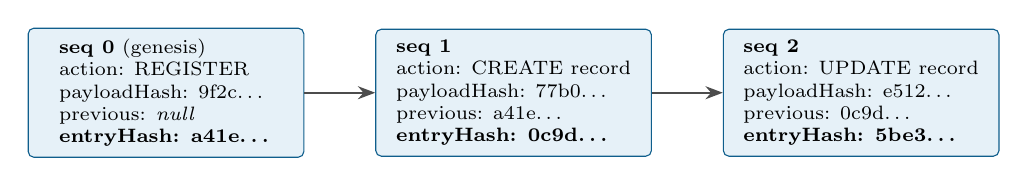
\begin{tikzpicture}[node distance=0.9cm,
  blk/.style={draw=brand,fill=brandlight,rounded corners=2pt,align=left,font=\scriptsize,minimum width=3.5cm,inner sep=4pt}]
  \node[blk] (e0) {\textbf{seq 0} (genesis)\\ action: REGISTER\\ payloadHash: 9f2c\ldots\\ previous: \textit{null}\\ \textbf{entryHash: a41e\ldots}};
  \node[blk,right=of e0] (e1) {\textbf{seq 1}\\ action: CREATE record\\ payloadHash: 77b0\ldots\\ previous: a41e\ldots\\ \textbf{entryHash: 0c9d\ldots}};
  \node[blk,right=of e1] (e2) {\textbf{seq 2}\\ action: UPDATE record\\ payloadHash: e512\ldots\\ previous: 0c9d\ldots\\ \textbf{entryHash: 5be3\ldots}};
  \draw[arr] (e0) -- (e1);
  \draw[arr] (e1) -- (e2);
\end{tikzpicture}
\caption{Three entries of the records chain}\label{fig:chain}
\end{figure}

Two kinds of tampering become detectable:

\begin{enumerate}
  \item \textbf{Editing a ledger entry.} If someone changes entry 1's action, its
    recomputed hash no longer equals its stored \code{entryHash}. If they also
    recompute and store the new hash, entry 2's \code{previousEntryHash} no
    longer matches. They would have to rewrite every later entry.
  \item \textbf{Editing the data itself.} Each entry stores the hash of the
    protected document's content (\code{payloadHash}) at that moment. If someone
    edits the medical record directly in MongoDB, the record's current hash no
    longer equals the hash the ledger last recorded for it, and they cannot fix
    the ledger without breaking the chain (point 1).
\end{enumerate}

\section{Two chains}

\begin{itemize}
  \item \textbf{records}: every create or change of clinical and financial data
    (users registered and verified, records, file attachments, consents,
    appointments, prescriptions, bills, claims, break-glass accesses).
  \item \textbf{access}: every allow or deny decision of the zero-trust layer.
\end{itemize}

They are independent sequences in the same collection, so the high-volume
access log does not slow down reads of a record's history.

\section{The entry: \file{src\codesl{}models\codesl{}LedgerEntry\codedot{}js}}

\begin{lstlisting}[language=JavaScript,caption={LedgerEntry schema (\file{src/models/LedgerEntry.js})}]
const ledgerEntrySchema = new mongoose.Schema({
  chain: { type: String, enum: ['records', 'access'], required: true },
  seq: { type: Number, required: true }, // position in the chain, starting at 0
  entityType: { type: String, required: true },
  entityId: { type: String, default: null },
  action: { type: String, required: true },
  actorId: { type: String, default: null },
  actorRole: { type: String, default: null },
  payloadHash: { type: String, default: null }, // SHA-256 of the entity's content at this moment
  meta: { type: mongoose.Schema.Types.Mixed, default: {} },
  timestamp: { type: Date, required: true },
  previousEntryHash: { type: String, default: null }, // null only for the genesis entry
  entryHash: { type: String, required: true },
}, { versionKey: false });

// The unique (chain, seq) index makes forking impossible: two writers that read
// the same "last entry" both try to insert seq N, and the second one fails.
ledgerEntrySchema.index({ chain: 1, seq: 1 }, { unique: true });
\end{lstlisting}

The application has no route that updates or deletes ledger entries. The only
code that writes them is \code{ledgerService.append}.

\section{Writing an entry: \file{src\codesl{}services\codesl{}ledgerService\codedot{}js}}

\begin{lstlisting}[language=JavaScript,caption={computeEntryHash and appendOnce (\file{src/services/ledgerService.js})}]
function computeEntryHash(entry) {
  return sha256(canonicalJSON({
    chain: entry.chain,
    seq: entry.seq,
    entityType: entry.entityType,
    entityId: entry.entityId ?? null,
    action: entry.action,
    actorId: entry.actorId ?? null,
    actorRole: entry.actorRole ?? null,
    payloadHash: entry.payloadHash ?? null,
    meta: entry.meta || {},
    timestamp: new Date(entry.timestamp).toISOString(),
    previousEntryHash: entry.previousEntryHash ?? null,
  }));
}

async function appendOnce({ chain, entityType, entityId, action, actorId, actorRole, payload, payloadHash, meta }) {
  const last = await LedgerEntry.findOne({ chain }).sort({ seq: -1 }).select('seq entryHash').lean();
  const entry = {
    chain,
    seq: last ? last.seq + 1 : 0,
    entityType,
    entityId: entityId ? String(entityId) : null,
    action,
    actorId: actorId ? String(actorId) : null,
    actorRole: actorRole || null,
    payloadHash: payloadHash || (payload !== undefined ? hashObject(payload) : null),
    // JSON round-trip drops undefined values, which MongoDB would otherwise
    // store as null and so change the hash on read-back.
    meta: meta ? JSON.parse(JSON.stringify(meta)) : {},
    timestamp: new Date(),
    previousEntryHash: last ? last.entryHash : null,
  };
  entry.entryHash = computeEntryHash(entry);
  return LedgerEntry.create(entry);
}
\end{lstlisting}

\begin{howto}
\begin{enumerate}
  \item Read the current head of the chain (highest \code{seq}).
  \item Build the new entry with \code{seq = head.seq + 1} and
    \code{previousEntryHash = head.entryHash}.
  \item Hash the entity's content (\code{payload}) with canonical JSON
    (Section~\ref{ch:foundation}), unless a hash was supplied (files supply the
    SHA-256 of their bytes).
  \item Hash every field of the entry, store it as \code{entryHash}, insert.
\end{enumerate}
The \code{meta} round-trip is a subtle fix: an \code{undefined} value would be
hashed as ``absent'' but stored by MongoDB as \code{null}, so the recomputed hash
on read-back would differ and the chain would appear broken.
\end{howto}

\subsection{Concurrency: two requests at once}

If two requests read the same head and both insert \code{seq = N}, the chain
would fork. Two mechanisms prevent this:

\begin{lstlisting}[language=JavaScript,caption={Serialised appends with retry (\file{src/services/ledgerService.js})}]
const queues = new Map();

function enqueue(chain, task) {
  const previous = queues.get(chain) || Promise.resolve();
  const next = previous.then(task, task);
  queues.set(chain, next.catch(() => {}));
  return next;
}

function append(params) {
  return enqueue(params.chain, async () => {
    for (let attempt = 0; attempt < 5; attempt += 1) {
      try {
        return await appendOnce(params);
      } catch (error) {
        if (error.code !== 11000) throw error; // not a sequence collision
      }
    }
    throw new Error('LEDGER_APPEND_CONFLICT');
  });
}
\end{lstlisting}

\begin{itemize}
  \item \textbf{Within one process}, appends to a chain form a promise queue:
    each waits for the previous one, so they read the head one after another.
  \item \textbf{Across processes} (several API instances), the unique
    \code{(chain, seq)} index makes the second insert fail with duplicate-key
    error 11000; the writer re-reads the head and retries.
\end{itemize}

\subsection{The shortcut used by every module}

\begin{lstlisting}[language=JavaScript,caption={recordEvent (\file{src/services/ledgerService.js})}]
function recordEvent({ entityType, entity, action, actor, meta, payloadHash }) {
  return append({
    chain: 'records',
    entityType,
    entityId: entity._id,
    action,
    actorId: actor ? actor.userId || actor._id : null,
    actorRole: actor ? actor.role : 'system',
    payload: typeof entity.ledgerPayload === 'function' ? entity.ledgerPayload() : undefined,
    payloadHash,
    meta,
  });
}
\end{lstlisting}

Each protected model defines \code{ledgerPayload()}: the fields whose integrity
matters. For a medical record:

\begin{lstlisting}[language=JavaScript,caption={What the ledger protects for a record (\file{src/models/MedicalRecord.js})}]
medicalRecordSchema.methods.ledgerPayload = function ledgerPayload() {
  return {
    patientId: this.patientId.toString(),
    doctorId: this.doctorId ? this.doctorId.toString() : null,
    recordType: this.recordType,
    title: this.title,
    description: this.description,
    diagnosis: this.diagnosis,
    findings: this.findings,
    attachments: this.attachments.map((a) => ({ fileId: a.fileId, sha256: a.sha256 })),
    version: this.version,
  };
};
\end{lstlisting}

Bookkeeping fields such as \code{updatedAt} or \code{ledgerEntryId} are left out
on purpose: they change for harmless reasons and would cause false alarms. The
same pattern exists on \code{Appointment}, \code{AccessGrant},
\code{Prescription}, \code{Bill} and \code{Claim}.

\section{Verifying}

\subsection{Walking a chain}

\begin{lstlisting}[language=JavaScript,caption={verifyChain (\file{src/services/ledgerService.js})}]
async function verifyChain(chain) {
  const cursor = LedgerEntry.find({ chain }).sort({ seq: 1 }).lean().cursor();
  let previous = null;
  let checked = 0;

  for await (const entry of cursor) {
    const expectedSeq = previous ? previous.seq + 1 : 0;
    if (entry.seq !== expectedSeq) {
      return { chain, valid: false, entriesChecked: checked, brokenAtSeq: expectedSeq, problem: 'missing_entry' };
    }
    if (entry.previousEntryHash !== (previous ? previous.entryHash : null)) {
      return { chain, valid: false, entriesChecked: checked, brokenAtSeq: entry.seq, problem: 'broken_link' };
    }
    if (computeEntryHash(entry) !== entry.entryHash) {
      return { chain, valid: false, entriesChecked: checked, brokenAtSeq: entry.seq, problem: 'entry_modified' };
    }
    previous = entry;
    checked += 1;
  }

  return { chain, valid: true, entriesChecked: checked, headHash: previous ? previous.entryHash : null };
}
\end{lstlisting}

A database cursor streams entries one by one, so even a large chain is verified
in constant memory. The three checks detect a deleted entry (a gap in
\code{seq}), a re-ordered or re-linked entry, and an edited entry.

\subsection{Checking a document against the ledger}

\begin{lstlisting}[language=JavaScript,caption={verifyEntity (\file{src/services/ledgerService.js})}]
async function verifyEntity(entityType, entity) {
  const latest = await LedgerEntry.findOne({
    chain: 'records', entityType, entityId: String(entity._id), payloadHash: { $ne: null },
    action: { $nin: ['FILE_ATTACHED', 'VIEW', 'BREAK_GLASS_ACCESS'] },
  }).sort({ seq: -1 }).lean();

  if (!latest) {
    return { entityId: String(entity._id), matches: false, reason: 'no_ledger_entry' };
  }
  const currentHash = hashObject(entity.ledgerPayload());
  return {
    entityId: String(entity._id),
    matches: currentHash === latest.payloadHash,
    currentHash,
    ledgerHash: latest.payloadHash,
    ledgerSeq: latest.seq,
  };
}
\end{lstlisting}

The most recent content-bearing entry for the document holds the hash of what
the document \emph{should} contain. Recompute the document's hash now; if they
differ, it was changed without going through the API. A document with no ledger
entry at all (inserted directly into the database) is also reported.

\subsection{The full audit: \code{GET \codesl{}api\codesl{}ledger\codesl{}verify}}

\begin{lstlisting}[language=JavaScript,caption={Full integrity audit (\file{src/modules/ledger/ledger.routes.js})}]
const PROTECTED = [
  { entityType: 'record', model: MedicalRecord, label: 'Medical records', describe: (d) => d.title },
  { entityType: 'prescription', model: Prescription, label: 'Prescriptions', describe: (d) => `${d.medication} ${d.dosage}` },
  { entityType: 'consent', model: AccessGrant, label: 'Consents', describe: (d) => `consent ${d.status}` },
  { entityType: 'appointment', model: Appointment, label: 'Appointments', describe: (d) => d.startTime.toISOString() },
  { entityType: 'claim', model: Claim, label: 'Insurance claims', describe: (d) => d.claimNumber },
  { entityType: 'bill', model: Bill, label: 'Bills', describe: (d) => d.billNumber },
];

router.get('/verify', asyncHandler(async (req, res) => {
  const started = Date.now();
  const chains = await Promise.all(['records', 'access'].map((c) => ledgerService.verifyChain(c)));

  const entities = [];
  for (const { entityType, model, label, describe } of PROTECTED) {
    const docs = await model.find();
    const results = await Promise.all(docs.map((doc) => ledgerService.verifyEntity(entityType, doc)));
    const tampered = results.map((r, i) => ({ ...r, name: describe(docs[i]) })).filter((r) => !r.matches);
    entities.push({
      entityType,
      label,
      checked: results.length,
      tampered: tampered.map((t) => ({ entityId: t.entityId, name: t.name, reason: t.reason || 'content_changed', ledgerSeq: t.ledgerSeq })),
    });
  }

  const valid = chains.every((c) => c.valid) && entities.every((e) => e.tampered.length === 0);
  res.json({ success: true, data: { valid, chains, entities, checkedAt: new Date(), durationMs: Date.now() - started } });
}));
\end{lstlisting}

This is what the admin's \textbf{Verify ledger} button calls, and what
\code{npm run ledger:verify} runs from the command line. For one record,
\code{GET \codesl{}api\codesl{}records\codesl{}:id\codesl{}verify} additionally re-reads every attached file from
GridFS and compares the SHA-256 of its bytes with the hash in the ledger
(Chapter~\ref{ch:records}).

\section{Demonstrating tamper detection}

\file{scripts\codesl{}tamper-demo\codedot{}js} plays a malicious insider with
direct database access:

\begin{lstlisting}[language=JavaScript,caption={The insider edit (\file{scripts/tamper-demo.js})}]
  const record = await MedicalRecord.findOne({ title: 'Stage 1 essential hypertension' });
  if (!record) throw new Error('Seeded record not found. Run "npm run seed -- --reset" first.');
  fs.writeFileSync(STATE, JSON.stringify({ recordId: record._id.toString(), original: record.diagnosis }));
  // updateOne on the raw collection: no API, no validation, no ledger entry. What an insider with DB access could do.
  await MedicalRecord.collection.updateOne({ _id: record._id }, { $set: { diagnosis: 'No hypertension. Patient healthy.' } });
\end{lstlisting}

\begin{lstlisting}[style=shell,caption={Running the demonstration}]
npm run demo:tamper            # change the diagnosis directly in MongoDB
npm run ledger:verify          # -> record ... TAMPERED: <id>  ...  TAMPERING DETECTED (exit 1)
npm run demo:tamper -- --restore
npm run ledger:verify          # -> LEDGER VALID
npm run demo:tamper -- --ledger    # rewrite a ledger entry -> chain "records": BROKEN (entry_modified)
\end{lstlisting}

The same result appears in the admin dashboard (Ledger $\to$ Verify ledger) and
on the patient's record (Verify integrity). The integration test in
\file{tests\codesl{}integration\codesl{}records\codedot{}test\codedot{}js} automates
exactly this scenario:

\begin{lstlisting}[language=JavaScript,caption={Tamper detection test (\file{tests/integration/records.test.js})}]
  test('editing a record directly in MongoDB (bypassing the API) is detected', async () => {
    const w = await world();
    await grantAccess(w);
    const created = await newRecord(w.doctor, w.patientUser._id);
    const id = created.body.data._id;

    await MedicalRecord.updateOne({ _id: id }, { $set: { diagnosis: 'Healthy, no hypertension' } });

    const verify = await as(w.doctor).get(`/api/records/${id}/verify`);
    expect(verify.body.data.intact).toBe(false);
    expect(verify.body.data.content.matches).toBe(false);

    const audit = await as(w.admin).get('/api/ledger/verify');
    expect(audit.body.data.valid).toBe(false);
    expect(audit.body.data.chains.every((c) => c.valid)).toBe(true); // the chain itself is intact
    const recordCheck = audit.body.data.entities.find((e) => e.entityType === 'record');
    expect(recordCheck.tampered.map((t) => t.entityId)).toEqual([id]);
  });
\end{lstlisting}

\section{Limits and how to close them}\label{sec:ledger-limits}

A hash chain proves that history is \emph{internally consistent}. An attacker
with full write access to MongoDB \emph{and} the patience to recompute every
hash after the edited point could produce a new, consistent chain. Two
inexpensive measures defeat that:

\begin{itemize}
  \item \textbf{Anchoring.} Periodically publish the head hash of each chain
    (\code{GET \codesl{}api\codesl{}ledger\codesl{}stats} returns it) somewhere the attacker cannot
    change: a signed email to auditors, a public timestamping service, or a
    public blockchain transaction. A rewritten chain will not reproduce a
    published head hash.
  \item \textbf{Separation of duties.} Run the API with a MongoDB user that may
    insert into \code{ledgerentries} but not update or delete.
\end{itemize}

Neither is implemented yet; both are listed in Chapter~\ref{ch:demo}. Moving to
Hyperledger Fabric later would replace \code{ledgerService} only: every caller
already goes through \code{append} and \code{recordEvent}.

%% =====================================================================
\chapter{Appointments}\label{ch:appointments}

\textbf{What it does.} Patients see a doctor's free slots and book one. Doctors
confirm, complete or mark no-show. Patients can reschedule; either side can
cancel. Completing a visit raises the bill.

\textbf{Files.} \file{src\codesl{}models\codesl{}Appointment\codedot{}js},
\file{src\codesl{}modules\codesl{}appointments\codesl{}slots\codedot{}js},
\file{src\codesl{}modules\codesl{}appointments\codesl{}appointments\codedot{}routes\codedot{}js},
\file{src\codesl{}modules\codesl{}users\codesl{}users\codedot{}routes\codedot{}js} (available slots).

\section{Generating slots from availability}

Doctors do not create slots one by one. Each doctor has an availability rule
(for example Monday--Friday, 9:00--17:00, 30-minute slots) and slots are
computed from it.

\begin{lstlisting}[language=JavaScript,caption={buildDaySlots and isValidSlot (\file{src/modules/appointments/slots.js})}]
function buildDaySlots(availability, dateString, maxAdvanceDays, now = new Date()) {
  const [year, month, day] = dateString.split('-').map(Number);
  const date = new Date(year, month - 1, day);
  if (Number.isNaN(date.getTime())) return [];

  const latest = new Date(now);
  latest.setDate(latest.getDate() + maxAdvanceDays);
  if (date > latest) return [];
  if (!availability.days.includes(date.getDay())) return [];

  const slots = [];
  const stepMs = availability.slotMinutes * 60 * 1000;
  const dayEnd = new Date(year, month - 1, day, availability.endHour, 0, 0, 0);
  for (let t = new Date(year, month - 1, day, availability.startHour, 0, 0, 0); t.getTime() + stepMs <= dayEnd.getTime(); t = new Date(t.getTime() + stepMs)) {
    if (t > now) slots.push({ start: t, end: new Date(t.getTime() + stepMs) });
  }
  return slots;
}

/** True when `start` is exactly one of the doctor's slot boundaries. */
function isValidSlot(availability, start, maxAdvanceDays, now = new Date()) {
  const dateString = `${start.getFullYear()}-${String(start.getMonth() + 1).padStart(2, '0')}-${String(start.getDate()).padStart(2, '0')}`;
  return buildDaySlots(availability, dateString, maxAdvanceDays, now).some((s) => s.start.getTime() === start.getTime());
}
\end{lstlisting}

\begin{howto}
\begin{itemize}
  \item Days outside the doctor's working days, or beyond the hospital's
    booking window (\code{maxAdvanceBookingDays}, an admin setting), have no
    slots.
  \item A slot is included only if it ends by \code{endHour}, and only if it is
    still in the future.
  \item \code{now} is a parameter so the unit tests can fix the clock.
  \item \code{isValidSlot} is what the booking endpoint uses: a client cannot
    book 9:07 or 3 a.m. by crafting a request, only a real slot.
\end{itemize}
\end{howto}

\code{GET \codesl{}api\codesl{}doctors\codesl{}:doctorId\codesl{}available-slots?date=YYYY-MM-DD} builds the
day's slots, then looks up appointments that already hold one of them, and marks
each slot \code{available: true\codesl{}false}. The patient's booking dialog shows taken
slots greyed out.

\section{Double-booking prevention}

Hiding taken slots in the interface is not enough: two patients can open the
dialog at the same moment and click the same slot. The guarantee is enforced by
the database:

\begin{lstlisting}[language=JavaScript,caption={Partial unique index (\file{src/models/Appointment.js})}]
  // True while the appointment occupies its slot. Cancelling sets it to false,
  // which frees the slot for someone else.
  holdsSlot: { type: Boolean, default: true },
}, { timestamps: true });

// Double-booking prevention at the database level: among appointments that
// hold their slot, a doctor can have only one per start time. Even two
// requests racing each other cannot both succeed.
appointmentSchema.index(
  { doctorId: 1, startTime: 1 },
  { unique: true, partialFilterExpression: { holdsSlot: true } }
);

appointmentSchema.pre('validate', function syncHoldsSlot(next) {
  this.holdsSlot = ACTIVE_STATUSES.includes(this.status);
  next();
});
\end{lstlisting}

\begin{howto}
A \emph{unique index} makes MongoDB reject a second document with the same
\code{(doctorId, startTime)}. A \emph{partial} index applies only to documents
matching a filter: here, those with \code{holdsSlot: true}. Pending, confirmed
and completed appointments hold their slot; cancelled and no-show ones do not.
So cancelling an appointment frees the slot automatically, while a race between
two bookings always ends with exactly one success. The \code{pre('validate')}
hook keeps \code{holdsSlot} in step with \code{status} on every save.
\end{howto}

\section{Booking: \code{POST \codesl{}api\codesl{}appointments}}

\begin{lstlisting}[language=JavaScript,caption={Booking a slot (\file{src/modules/appointments/appointments.routes.js})}]
router.post('/', requireRole('patient'),
  validate({ body: Joi.object({
    doctorId: objectId().required(),
    startTime: Joi.date().iso().greater('now').required(),
    type: Joi.string().valid('consultation', 'follow_up', 'checkup').default('consultation'),
    reason: Joi.string().trim().min(3).max(500).required(),
  }) }),
  asyncHandler(async (req, res) => {
    const { doctorId, startTime, type, reason } = req.body;
    const doctor = await User.findOne({ _id: doctorId, role: 'doctor', approvalStatus: 'approved', isActive: true });
    if (!doctor) throw notFound('Doctor not found');

    const settings = await HospitalSettings.getSingleton();
    const start = new Date(startTime);
    if (!isValidSlot(doctor.doctorProfile.availability, start, settings.maxAdvanceBookingDays)) {
      throw badRequest('That time is not one of the doctor\'s available slots');
    }

    let appointment;
    try {
      appointment = await Appointment.create({
        patientId: req.user.userId,
        doctorId,
        startTime: start,
        endTime: new Date(start.getTime() + doctor.doctorProfile.availability.slotMinutes * 60000),
        type,
        reason,
      });
    } catch (error) {
      if (error.code === 11000) throw conflict('This slot has just been booked. Please choose another time.', 'SLOT_TAKEN');
      throw error;
    }

    await recordAppointmentEvent(appointment, 'CREATE', req);
    await notificationService.notify(doctorId, {
      type: 'info', title: 'New appointment request',
      message: `A patient requested a ${type.replace('_', '-')} on ${fmt(start)}: "${reason}"`, page: 'appointments',
    });
    // ... 201 with the populated appointment
\end{lstlisting}

\begin{howto}
Only verified, active doctors can be booked. The duplicate-key error (11000)
from the unique index is translated into a friendly 409 \code{SLOT\_TAKEN}; the
frontend shows the message and reloads the slot grid. Every booking is a ledger
entry and a notification for the doctor.
\end{howto}

\section{Status changes, rescheduling and cancelling}

\begin{figure}[H]
\centering
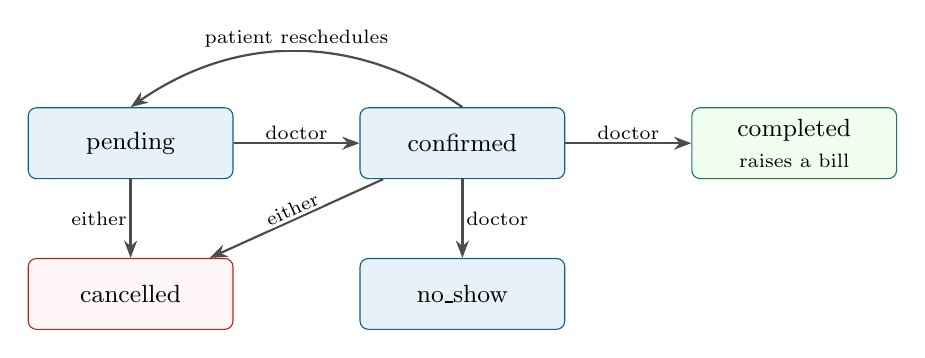
\begin{tikzpicture}[node distance=1.0cm and 1.6cm]
  \node[box] (p) {pending};
  \node[box,right=of p] (c) {confirmed};
  \node[box,right=of c,draw=okgreen,fill=green!6] (d) {completed\\\scriptsize raises a bill};
  \node[box,below=of c] (n) {no\_show};
  \node[box,below=of p,draw=badred,fill=red!3] (x) {cancelled};
  \draw[arr] (p) -- node[lbl,above]{doctor} (c);
  \draw[arr] (c) -- node[lbl,above]{doctor} (d);
  \draw[arr] (c) -- node[lbl,right]{doctor} (n);
  \draw[arr] (p) -- node[lbl,left]{either} (x);
  \draw[arr] (c) -- node[lbl,above,sloped]{either} (x);
  \draw[arr] (c.north) to[bend right=35] node[lbl,above]{patient reschedules} (p.north);
\end{tikzpicture}
\caption{Appointment states}\label{fig:appt-states}
\end{figure}

\begin{lstlisting}[language=JavaScript,caption={Allowed doctor transitions (\file{appointments.routes.js})}]
const DOCTOR_TRANSITIONS = { pending: ['confirmed'], confirmed: ['completed', 'no_show'] };
// ...
      const allowed = DOCTOR_TRANSITIONS[appointment.status] || [];
      if (!allowed.includes(req.body.status)) {
        throw conflict(`Cannot change an appointment from "${appointment.status}" to "${req.body.status}"`, 'INVALID_TRANSITION');
      }
      if (req.body.status === 'completed' && appointment.startTime > new Date()) {
        throw conflict('An appointment cannot be completed before it starts', 'INVALID_TRANSITION');
      }
      appointment.status = req.body.status;
      if (req.body.notes !== undefined) appointment.notes = req.body.notes;
      await appointment.save();
      await recordAppointmentEvent(appointment, req.body.status.toUpperCase(), req);
      // ... notify the patient
      if (req.body.status === 'completed') {
        const doctor = await User.findById(appointment.doctorId);
        await createBillForAppointment(appointment, doctor, req.user);
      }
\end{lstlisting}

\begin{itemize}
  \item \textbf{Who may do what} is checked on the server: only the doctor
    changes status (and only once approved), only the patient reschedules.
  \item \textbf{Rescheduling} (\code{PATCH} with \code{startTime}) re-runs
    \code{isValidSlot}, moves the appointment, sets it back to \emph{pending}
    (the doctor must confirm the new time) and catches the same 11000 error if
    the new slot was just taken.
  \item \textbf{Cancelling} (\code{DELETE}) is allowed for pending and confirmed
    appointments; the record stays (with who cancelled and why) and the slot is
    freed through \code{holdsSlot}.
  \item An appointment that is not yours returns \textbf{404}, not 403, so
    appointment ids cannot be probed.
\end{itemize}

%% =====================================================================
\chapter{Medical Records, Consent and Files}\label{ch:records}

This is the heart of the system: who may see a patient's medical data, how
records are written and amended, and how attached files are stored and proven
unchanged.

\section{Consent model}

A patient's consent is an \code{AccessGrant} document linking one patient and
one doctor, with a status and an expiry date.

\begin{lstlisting}[language=JavaScript,caption={AccessGrant (\file{src/models/AccessGrant.js})}]
const accessGrantSchema = new mongoose.Schema({
  patientId: { type: mongoose.Schema.Types.ObjectId, ref: 'User', required: true, index: true },
  doctorId: { type: mongoose.Schema.Types.ObjectId, ref: 'User', required: true, index: true },
  status: { type: String, enum: ['requested', 'active', 'denied', 'revoked'], default: 'requested' },
  purpose: { type: String, trim: true, default: '' },
  requestedBy: { type: String, enum: ['doctor', 'patient'], required: true },
  grantedAt: { type: Date, default: null },
  expiresAt: { type: Date, default: null },
  revokedAt: { type: Date, default: null },
  ledgerEntryId: { type: String, default: null },
}, { timestamps: true });

/** The status the user sees: an active grant past its expiry shows as "expired". */
accessGrantSchema.methods.effectiveStatus = function effectiveStatus(now = new Date()) {
  if (this.status === 'active' && (!this.expiresAt || this.expiresAt <= now)) return 'expired';
  return this.status;
};
\end{lstlisting}

\begin{figure}[H]
\centering
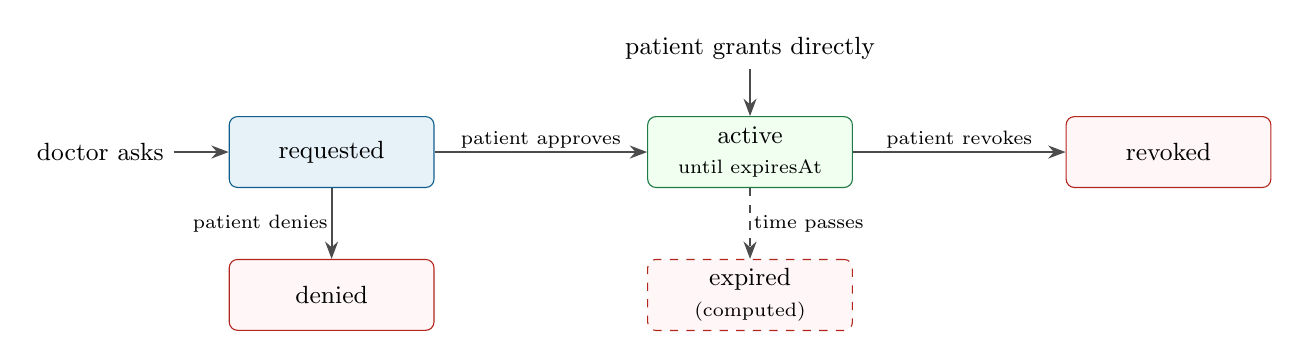
\begin{tikzpicture}[node distance=0.9cm and 2.7cm]
  \node[box] (r) {requested};
  \node[box,right=of r,draw=okgreen,fill=green!6] (a) {active\\\scriptsize until expiresAt};
  \node[box,below=of r,draw=badred,fill=red!3] (d) {denied};
  \node[box,right=of a,draw=badred,fill=red!3] (v) {revoked};
  \node[box,below=of a,dashedbox] (e) {expired\\\scriptsize (computed)};
  \node[left=0.7cm of r,font=\small] (start) {doctor asks};
  \draw[arr] (start) -- (r);
  \draw[arr] (r) -- node[lbl,above]{patient approves} (a);
  \draw[arr] (r) -- node[lbl,left]{patient denies} (d);
  \draw[arr] (a) -- node[lbl,above]{patient revokes} (v);
  \draw[arr,dashed] (a) -- node[lbl,right]{time passes} (e);
  \node[above=0.6cm of a,font=\small] (g) {patient grants directly};
  \draw[arr] (g) -- (a);
\end{tikzpicture}
\caption{Consent lifecycle}\label{fig:consent}
\end{figure}

\begin{howto}
``Expired'' is never written to the database: it is computed from
\code{expiresAt} every time. That way a grant expires at exactly the right
moment, with no background job. Every transition (\code{REQUEST\_ACCESS},
\code{GRANT\_ACCESS}, \code{APPROVE}, \code{DENY}, \code{REVOKE}) is a ledger
entry, and the other party is notified.
\end{howto}

\begin{lstlisting}[language=JavaScript,caption={A patient grants access directly (\file{src/modules/consents/consents.routes.js})}]
    const settings = await HospitalSettings.getSingleton();
    const days = req.body.durationDays || settings.defaultConsentDays;

    // Replace any pending request or existing active grant with this one.
    await AccessGrant.updateMany(
      { patientId: req.user.userId, doctorId: doctor._id, status: { $in: ['requested', 'active'] } },
      { $set: { status: 'revoked', revokedAt: new Date() } }
    );
    const now = new Date();
    const grant = await AccessGrant.create({
      patientId: req.user.userId, doctorId: doctor._id, status: 'active', purpose: req.body.purpose,
      requestedBy: 'patient', grantedAt: now, expiresAt: new Date(now.getTime() + days * 86400000),
    });
    await ledger(grant, 'GRANT_ACCESS', req);
\end{lstlisting}

\section{The consent gate: \file{src\codesl{}services\codesl{}consentService\codedot{}js}}

Every module that returns patient data (records, files, vitals,
prescriptions) calls one function:

\begin{lstlisting}[language=JavaScript,caption={assertCanAccessPatient (\file{src/services/consentService.js})}]
async function hasActiveGrant(doctorId, patientId, now = new Date()) {
  const grant = await AccessGrant.exists({
    doctorId, patientId, status: 'active', expiresAt: { $gt: now },
  });
  return Boolean(grant);
}

async function assertCanAccessPatient(req, patientId, { purpose = 'view medical data' } = {}) {
  const { userId, role } = req.user;
  const pid = String(patientId);

  if (role === 'patient') {
    if (userId === pid) return { via: 'owner' };
    throw forbidden('Patients can only access their own data.', 'NOT_OWNER');
  }

  if (role === 'doctor' && await hasActiveGrant(userId, pid)) {
    return { via: 'consent' };
  }

  if (req.policy?.breakGlass) {
    await ledgerService.append({
      chain: 'records',
      entityType: 'patient',
      entityId: pid,
      action: 'BREAK_GLASS_ACCESS',
      actorId: userId,
      actorRole: role,
      meta: { reason: req.policy.breakGlassReason, purpose, path: req.originalUrl },
    });
    await notificationService.notify(pid, {
      type: 'danger',
      title: 'Emergency access to your records',
      message: `A ${role} accessed your records under emergency (break-glass) access. Reason given: "${req.policy.breakGlassReason}". This access is logged in the ledger.`,
      page: 'permissions',
    });
    await notificationService.notifyRole('admin', { /* ... 'Break-glass access used' */ });
    return { via: 'break_glass' };
  }

  throw forbidden('No active consent from this patient. Request access, or use emergency access if this is an emergency.', 'CONSENT_REQUIRED');
}
\end{lstlisting}

\begin{howto}
\begin{itemize}
  \item A patient sees only their own data.
  \item A doctor needs a grant that is \code{active} \emph{and} not past
    \code{expiresAt}, checked in the same query.
  \item Admins run the system but do not treat patients: they have no consent
    path, only audited break-glass.
  \item The return value says \emph{how} access was obtained. The records list
    passes it to the frontend (\code{meta.accessVia}), which shows a red
    emergency banner when it is \code{break\_glass}.
\end{itemize}
\end{howto}

\section{Records: \file{src\codesl{}modules\codesl{}records\codesl{}records\codedot{}routes\codedot{}js}}

\begin{lstlisting}[language=JavaScript,caption={Record policies and creation (\file{records.routes.js})}]
// Medical data is high-sensitivity: it needs the higher trust bar, and doctors
// or admins may override consent in an emergency (break-glass, audited).
const readPolicy = requireRole('patient', 'doctor', {
  minTrustScore: config.security.highSensitivityTrustScore, allowBreakGlass: true,
});
const writePolicy = requireRole('patient', 'doctor', { minTrustScore: config.security.highSensitivityTrustScore });
// ...
    if (role === 'patient') {
      patientId = userId;
      if (req.body.recordType !== 'patient_upload') throw forbidden('Patients can only add their own uploaded documents');
    } else {
      if (!patientId) throw badRequest('patientId is required');
      if (req.body.recordType === 'patient_upload') throw badRequest('Choose a clinical record type');
      await consentService.assertCanAccessPatient(req, patientId, { purpose: 'create record' });
    }

    const record = await MedicalRecord.create({
      ...req.body,
      patientId,
      doctorId: role === 'doctor' ? userId : null,
    });
    const entry = await ledgerService.recordEvent({ entityType: 'record', entity: record, action: 'CREATE', actor: req.user });
    record.ledgerEntryId = entry._id.toString();
    await record.save();
\end{lstlisting}

Note that the \emph{write} policy does not allow break-glass: emergency access
is for reading a history, not for writing records without consent.

\subsection{Amending a record}

\begin{lstlisting}[language=JavaScript,caption={Versioned amendment (\file{records.routes.js})}]
    const record = await loadRecordWithAccess(req);
    if (!record.doctorId || record.doctorId.toString() !== req.user.userId) {
      throw forbidden('Only the doctor who wrote this record can amend it');
    }
    Object.assign(record, req.body);
    record.version += 1;
    const entry = await ledgerService.recordEvent({
      entityType: 'record', entity: record, action: 'UPDATE', actor: req.user, meta: { version: record.version },
    });
    record.ledgerEntryId = entry._id.toString();
    await record.save();
\end{lstlisting}

Records are never edited silently: the version number goes up and a new
\code{UPDATE} entry, containing the hash of the new content, is chained. The
ledger history (\code{GET \codesl{}api\codesl{}records\codesl{}:id\codesl{}ledger-history}) therefore shows
every version, who made it and when, with the actor's name resolved for display.

\section{Files: GridFS with hashes in the ledger}

\begin{lstlisting}[language=JavaScript,caption={Upload limits (\file{records.routes.js})}]
const ALLOWED_TYPES = ['application/pdf', 'image/png', 'image/jpeg', 'text/plain'];
const upload = multer({
  storage: multer.memoryStorage(),
  limits: { fileSize: config.files.maxBytes, files: 1 },
  fileFilter: (req, file, cb) => (ALLOWED_TYPES.includes(file.mimetype)
    ? cb(null, true)
    : cb(badRequest('Only PDF, PNG, JPEG and plain-text files are accepted'))),
});
\end{lstlisting}

\begin{lstlisting}[language=JavaScript,caption={Storing a file and anchoring its hash (\file{records.routes.js})}]
    const sha256 = crypto.createHash('sha256').update(req.file.buffer).digest('hex');
    const fileId = await new Promise((resolve, reject) => {
      const stream = getBucket().openUploadStream(req.file.originalname, {
        metadata: { recordId: record._id.toString(), patientId: record.patientId.toString(), sha256, contentType: req.file.mimetype, uploadedBy: req.user.userId },
      });
      Readable.from(req.file.buffer).pipe(stream).on('error', reject).on('finish', () => resolve(stream.id.toString()));
    });

    record.attachments.push({
      fileId, filename: req.file.originalname, contentType: req.file.mimetype, size: req.file.size, sha256, uploadedBy: req.user.userId,
    });
    await ledgerService.append({
      chain: 'records', entityType: 'file', entityId: fileId, action: 'FILE_ATTACHED',
      actorId: req.user.userId, actorRole: req.user.role, payloadHash: sha256,
      meta: { recordId: record._id.toString(), filename: req.file.originalname, size: req.file.size },
    });
    // The record's own content (its attachment list) changed too, so chain a new version.
    record.version += 1;
    const entry = await ledgerService.recordEvent({ entityType: 'record', entity: record, action: 'UPDATE', actor: req.user, meta: { attached: fileId } });
\end{lstlisting}

\begin{howto}
\begin{enumerate}
  \item multer accepts one file, checks its type and size, and keeps it in
    memory (at most 10\,MB).
  \item The SHA-256 of the bytes is computed \emph{before} storage.
  \item The bytes stream into GridFS, which splits them into 255\,kB chunks.
  \item Two ledger entries: \code{FILE\_ATTACHED} with the file's hash (the
    place where the paper put the IPFS content hash), and a record
    \code{UPDATE}, because the record's attachment list is part of its protected
    content.
\end{enumerate}
\end{howto}

\subsection{Downloading}

\begin{lstlisting}[language=JavaScript,caption={Consent-gated download (\file{src/modules/records/files.routes.js})}]
    const record = await MedicalRecord.findOne({ 'attachments.fileId': req.params.fileId });
    if (!record) throw notFound('File not found');
    await consentService.assertCanAccessPatient(req, record.patientId, { purpose: 'download file' });

    const attachment = record.attachments.find((a) => a.fileId === req.params.fileId);
    res.set({
      'Content-Type': attachment.contentType,
      'Content-Length': attachment.size,
      'Content-Disposition': `inline; filename="${attachment.filename.replace(/"/g, '')}"`,
      'X-Content-SHA256': attachment.sha256,
      'Cache-Control': 'private, no-store',
    });
    getBucket().openDownloadStream(new mongoose.Types.ObjectId(req.params.fileId))
      .on('error', () => { if (!res.headersSent) res.status(404).end(); else res.end(); })
      .pipe(res);
\end{lstlisting}

A file is reachable only through its record, so it inherits exactly the
record's access rules. \code{no-store} keeps medical files out of shared
caches. The expected hash travels in \code{X-Content-SHA256} so a client can
check the download itself.

\subsection{Verifying a record and its files}

\begin{lstlisting}[language=JavaScript,caption={Per-record integrity check (\file{records.routes.js})}]
  const record = await loadRecordWithAccess(req);
  const content = await ledgerService.verifyEntity('record', record);

  const files = [];
  for (const attachment of record.attachments) {
    const hash = crypto.createHash('sha256');
    try {
      await new Promise((resolve, reject) => {
        getBucket().openDownloadStream(new mongoose.Types.ObjectId(attachment.fileId))
          .on('data', (chunk) => hash.update(chunk)).on('error', reject).on('end', resolve);
      });
      const actual = hash.digest('hex');
      files.push({ fileId: attachment.fileId, filename: attachment.filename, matches: actual === attachment.sha256, expected: attachment.sha256, actual });
    } catch (error) {
      files.push({ fileId: attachment.fileId, filename: attachment.filename, matches: false, error: 'file_missing' });
    }
  }
  const intact = content.matches && files.every((f) => f.matches);
\end{lstlisting}

The \emph{Verify integrity} button on a record (patient and doctor dashboards)
calls this. It re-hashes the record's content and every stored file, streaming
the bytes so large files do not fill memory, and reports which part, if any, no
longer matches the ledger.

%% =====================================================================
\chapter{Prescriptions, Vital Signs and IoT Devices}\label{ch:rxvitals}

\section{Prescriptions}

\textbf{Files.} \file{src\codesl{}models\codesl{}Prescription\codedot{}js},
\file{src\codesl{}modules\codesl{}prescriptions\codesl{}prescriptions\codedot{}routes\codedot{}js}.

A doctor with the patient's consent prescribes a medication with dosage,
frequency, instructions, dates and a number of allowed refills. The patient sees
active and past medications and can request a refill; the doctor approves or
denies it.

\begin{lstlisting}[language=JavaScript,caption={Refill request rules (\file{prescriptions.routes.js})}]
router.post('/:id/refill-request', requireRole('patient'), validate(idParam), asyncHandler(async (req, res) => {
  const rx = await Prescription.findOne({ _id: req.params.id, patientId: req.user.userId });
  if (!rx) throw notFound('Prescription not found');
  if (rx.status !== 'active') throw conflict('Only active prescriptions can be refilled', 'INVALID_TRANSITION');
  if (rx.refillRequest.status === 'pending') throw conflict('A refill request is already pending', 'ALREADY_PENDING');
  if (rx.refillsUsed >= rx.refillsAllowed) throw conflict('No refills remain on this prescription. Book an appointment for a new one.', 'NO_REFILLS');

  rx.refillRequest = { status: 'pending', requestedAt: new Date(), decidedAt: null };
  await chain(rx, 'REFILL_REQUESTED', req);
  await notificationService.notify(rx.doctorId, {
    type: 'warning', title: 'Refill request', message: `A patient requested a refill of ${rx.medication} ${rx.dosage}.`, page: 'prescriptions',
  });
  res.json({ success: true, message: 'Refill requested', data: rx });
}));
\end{lstlisting}

\begin{lstlisting}[language=JavaScript,caption={The doctor decides (\file{prescriptions.routes.js})}]
    if (action === 'approve_refill' || action === 'deny_refill') {
      if (rx.refillRequest.status !== 'pending') throw conflict('There is no pending refill request', 'INVALID_TRANSITION');
      const approved = action === 'approve_refill';
      rx.refillRequest.status = approved ? 'approved' : 'denied';
      rx.refillRequest.decidedAt = new Date();
      if (approved) rx.refillsUsed += 1;
      await chain(rx, approved ? 'REFILL_APPROVED' : 'REFILL_DENIED', req);
      // ... notify the patient
    } else {
      if (rx.status !== 'active') throw conflict(`The prescription is already ${rx.status}`, 'INVALID_TRANSITION');
      rx.status = action === 'complete' ? 'completed' : 'cancelled';
      await chain(rx, action === 'complete' ? 'COMPLETE' : 'CANCEL', req);
    }
\end{lstlisting}

The doctor can only act on prescriptions they wrote (the query includes
\code{doctorId}). All rule violations return 409 with a precise message, which
the dashboard shows as-is. Every change is chained in the ledger, so the
dispensing history of a controlled drug can be audited.

\section{Vital signs}

\textbf{Files.} \file{src\codesl{}models\codesl{}VitalReading\codedot{}js}, \file{src\codesl{}models\codesl{}Device\codedot{}js},
\file{src\codesl{}modules\codesl{}vitals\codesl{}vitals\codedot{}routes\codedot{}js}.

\begin{lstlisting}[language=JavaScript,caption={Normal ranges and the abnormal check (\file{src/models/VitalReading.js})}]
const VITAL_RANGES = {
  heartRate: { min: 50, max: 110, unit: 'bpm', label: 'Heart rate' },
  systolic: { min: 90, max: 140, unit: 'mmHg', label: 'Systolic BP' },
  diastolic: { min: 60, max: 90, unit: 'mmHg', label: 'Diastolic BP' },
  spo2: { min: 94, max: 100, unit: '%', label: 'Blood oxygen' },
  temperature: { min: 36.1, max: 37.8, unit: 'C', label: 'Temperature' },
  glucose: { min: 70, max: 180, unit: 'mg/dL', label: 'Blood glucose' },
};

/** Returns the names of the fields in `reading` that fall outside VITAL_RANGES. */
function findAbnormal(reading) {
  return Object.entries(VITAL_RANGES)
    .filter(([field, range]) => reading[field] !== null && reading[field] !== undefined
      && (reading[field] < range.min || reading[field] > range.max))
    .map(([field]) => field);
}
\end{lstlisting}

(The temperature unit in the source is the degree sign, \textdegree C.) The
ranges are sent to the frontend with every vitals response, so the charts and
tiles colour values with the same thresholds the server uses for alerts.

\begin{lstlisting}[language=JavaScript,caption={Saving a reading and raising alerts (\file{vitals.routes.js})}]
async function saveReading(patientId, values, source, deviceId = null) {
  const reading = await VitalReading.create({
    patientId, deviceId, source, ...values, abnormal: findAbnormal(values), recordedAt: values.recordedAt || new Date(),
  });

  if (reading.abnormal.length) {
    const details = reading.abnormal.map((f) => `${VITAL_RANGES[f].label} ${reading[f]} ${VITAL_RANGES[f].unit}`).join(', ');
    const patient = await User.findById(patientId).select('fullName');
    const doctors = await AccessGrant.find({ patientId, status: 'active', expiresAt: { $gt: new Date() } }).distinct('doctorId');
    await notificationService.notify(patientId, {
      type: 'danger', title: 'Abnormal vital sign', message: `Out of normal range: ${details}.`, page: 'metrics',
    });
    await notificationService.notify(doctors, {
      type: 'danger', title: `Vitals alert: ${patient.fullName}`, message: `Out of normal range: ${details}.`, page: 'iot',
    });
  }
  return reading;
}
\end{lstlisting}

Alerts go to the patient and to every doctor who \emph{currently} has consent:
the consent model decides who is told, not just who can look.

\section{IoT devices}

\subsection{Registration and keys}

An admin registers a device (serial number, type, patient). The server generates
a random API key, stores only its SHA-256, and shows the key once:

\begin{lstlisting}[language=JavaScript,caption={Device model (\file{src/models/Device.js})}]
const deviceSchema = new mongoose.Schema({
  serialNumber: { type: String, required: true, unique: true, trim: true },
  name: { type: String, required: true, trim: true },
  type: { type: String, enum: ['heart_monitor', 'bp_monitor', 'pulse_oximeter', 'thermometer', 'multi_parameter'], required: true },
  patientId: { type: mongoose.Schema.Types.ObjectId, ref: 'User', required: true, index: true },
  apiKeyHash: { type: String, required: true, unique: true },
  status: { type: String, enum: ['active', 'inactive'], default: 'active' },
  lastSeenAt: { type: Date, default: null },
  registeredBy: { type: mongoose.Schema.Types.ObjectId, ref: 'User', required: true },
}, { timestamps: true });
\end{lstlisting}

\subsection{Ingestion}

\begin{lstlisting}[language=JavaScript,caption={POST /api/devices/readings (\file{vitals.routes.js})}]
router.post('/devices/readings', validate({ body: readingSchema }), asyncHandler(async (req, res) => {
  const key = req.get('x-device-key');
  if (!key) throw unauthorized('Device key required', 'NO_DEVICE_KEY');
  const device = await Device.findOne({ apiKeyHash: crypto.createHash('sha256').update(key).digest('hex') });
  if (!device || device.status !== 'active') throw unauthorized('Unknown or inactive device', 'INVALID_DEVICE');

  const reading = await saveReading(device.patientId, req.body, 'device', device._id);
  device.lastSeenAt = new Date();
  await device.save();
  res.status(201).json({ success: true, data: { readingId: reading._id, abnormal: reading.abnormal } });
}));
\end{lstlisting}

\begin{howto}
A device is not a user: it has no password, no OTP and no JWT. It proves its
identity with its key, and the key's hash identifies the device and therefore
the patient. A device cannot choose which patient a reading belongs to, so a
stolen key can only add readings for one patient, and the admin can deactivate
the device at once. The Joi schema rejects physiologically impossible values
(for example a heart rate of 400).
\end{howto}

\subsection{The doctor's live monitor}

\code{GET \codesl{}api\codesl{}vitals\codesl{}monitor} returns, for every patient who currently allows
this doctor in, the latest reading and the patient's devices with their
\code{lastSeenAt}. The doctor's \emph{IoT Monitoring} page polls it, so readings
from devices (or from the simulator) appear within seconds.

\subsection{The simulator}

\file{scripts\codesl{}iot-simulator\codedot{}js} stands in for real hardware. It
reads the seeded device keys from \file{scripts\codesl{}\codedot{}demo-devices\codedot{}json} (git-ignored)
and posts readings to the real ingestion endpoint:

\begin{lstlisting}[language=JavaScript,caption={Simulated readings (\file{scripts/iot-simulator.js})}]
function readingFor(device) {
  if (spike) {
    return device.type === 'pulse_oximeter'
      ? { heartRate: Math.round(vary(128, 4)), spo2: Math.round(vary(89, 1)) }
      : { heartRate: Math.round(vary(124, 4)), systolic: Math.round(vary(168, 4)), diastolic: Math.round(vary(104, 3)), spo2: 96, temperature: vary(37.2, 0.2) };
  }
  if (device.type === 'pulse_oximeter') return { heartRate: Math.round(vary(80, 6)), spo2: Math.round(vary(97, 1)) };
  return {
    heartRate: Math.round(vary(74, 6)), systolic: Math.round(vary(126, 5)), diastolic: Math.round(vary(81, 3)),
    spo2: Math.round(vary(97.5, 1)), temperature: vary(36.8, 0.2),
  };
}
\end{lstlisting}

With \code{--spike}, the first reading from each device is clearly abnormal
(blood pressure around 168/104, SpO\textsubscript{2} around 89\%) and later ones
are normal again: a single burst that demonstrates the alert path end to end.

%% =====================================================================
\chapter{Billing and Insurance Claims}\label{ch:billing}

\textbf{Files.} \file{src\codesl{}models\codesl{}Bill\codedot{}js}, \file{src\codesl{}models\codesl{}Claim\codedot{}js},
\file{src\codesl{}modules\codesl{}billing\codesl{}}, \file{src\codesl{}modules\codesl{}claims\codesl{}claims\codedot{}routes\codedot{}js}.

\section{Bills}

A bill is never typed in by hand. It is raised automatically when a doctor
marks an appointment \emph{completed}, at the doctor's consultation fee:

\begin{lstlisting}[language=JavaScript,caption={createBillForAppointment (\file{src/modules/billing/billing.service.js})}]
/** Human-readable unique number, e.g. "B-20261027-3FA9C1". */
function makeNumber(prefix) {
  const d = new Date();
  const date = `${d.getFullYear()}${String(d.getMonth() + 1).padStart(2, '0')}${String(d.getDate()).padStart(2, '0')}`;
  return `${prefix}-${date}-${crypto.randomBytes(3).toString('hex').toUpperCase()}`;
}

/** Raises the consultation bill when a doctor completes an appointment. */
async function createBillForAppointment(appointment, doctor, actor) {
  const bill = await Bill.create({
    billNumber: makeNumber('B'),
    patientId: appointment.patientId,
    doctorId: appointment.doctorId,
    appointmentId: appointment._id,
    description: `Consultation with Dr. ${doctor.fullName} (${doctor.doctorProfile.specialization || 'General'})`,
    amount: doctor.doctorProfile.consultationFee,
  });
  await ledgerService.recordEvent({ entityType: 'bill', entity: bill, action: 'CREATE', actor });
  // ... notify the patient: "A bill of Rs. ... was raised"
  return bill;
}
\end{lstlisting}

\begin{figure}[H]
\centering
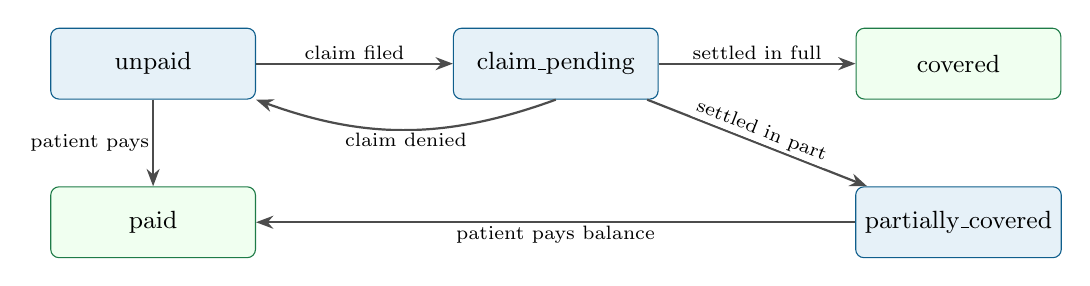
\begin{tikzpicture}[node distance=1.1cm and 2.5cm]
  \node[box] (u) {unpaid};
  \node[box,right=of u] (cp) {claim\_pending};
  \node[box,right=of cp,draw=okgreen,fill=green!6] (cov) {covered};
  \node[box,below=of cov] (pc) {partially\_covered};
  \node[box,below=of u,draw=okgreen,fill=green!6] (paid) {paid};
  \draw[arr] (u) -- node[lbl,above]{claim filed} (cp);
  \draw[arr] (cp) -- node[lbl,above]{settled in full} (cov);
  \draw[arr] (cp) -- node[lbl,above,sloped]{settled in part} (pc);
  \draw[arr] (cp.south) to[bend left=20] node[lbl,below]{claim denied} (u.south east);
  \draw[arr] (u) -- node[lbl,left]{patient pays} (paid);
  \draw[arr] (pc) -- node[lbl,below]{patient pays balance} (paid);
\end{tikzpicture}
\caption{Bill states}\label{fig:bill}
\end{figure}

\code{POST \codesl{}api\codesl{}bills\codesl{}:id\codesl{}pay} records that the patient paid the outstanding
balance (amount minus what insurance covered). There is no payment gateway:
the endpoint records the payment and chains it in the ledger
(\code{PAYMENT\_RECORDED}). Connecting a real gateway is listed as future work.

\section{Claims}

\subsection{Filing a claim}

\begin{lstlisting}[language=JavaScript,caption={POST /api/claims (\file{claims.routes.js})}]
    const patient = await User.findById(req.user.userId);
    const { insuranceProvider, policyNumber } = patient.patientProfile;
    if (!insuranceProvider || !policyNumber) {
      throw badRequest('Add your insurance provider and policy number in Settings before filing a claim');
    }
    const bill = await Bill.findOne({ _id: req.body.billId, patientId: patient._id });
    if (!bill) throw notFound('Bill not found');
    if (bill.status !== 'unpaid') throw conflict(`This bill is ${bill.status.replace('_', ' ')} and cannot be claimed`, 'INVALID_TRANSITION');

    const claim = new Claim({
      claimNumber: makeNumber('CLM'),
      patientId: patient._id,
      billId: bill._id,
      insuranceProvider,
      policyNumber,
      amount: bill.amount,
      description: req.body.description || bill.description,
      history: [{ status: 'submitted', by: req.user.userId, byRole: 'patient', note: 'Claim submitted' }],
    });
    await chain(claim, 'SUBMIT', req);
    bill.status = 'claim_pending';
    await bill.save();
    // ... ledger entry for the bill, notify the insurer's agents
\end{lstlisting}

\begin{howto}
A claim always refers to a real bill of the same patient, for the bill's exact
amount; the patient cannot invent an amount. The provider and policy number come
from the patient's profile. Only unpaid bills can be claimed, and filing moves
the bill to \code{claim\_pending} so it cannot be claimed twice or paid while
under review. Only agents of that insurer are notified.
\end{howto}

\subsection{The claim state machine}

\begin{lstlisting}[language=JavaScript,caption={Allowed transitions (\file{src/models/Claim.js})}]
const CLAIM_TRANSITIONS = {
  submitted: ['under_review'],
  under_review: ['approved', 'denied'],
  approved: ['settled'],
  denied: [],
  settled: [],
};
\end{lstlisting}

\begin{figure}[H]
\centering
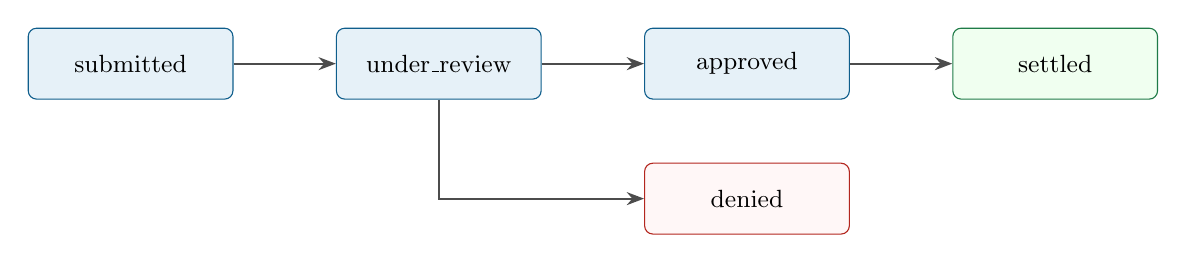
\begin{tikzpicture}[node distance=0.8cm and 1.3cm]
  \node[box] (s) {submitted};
  \node[box,right=of s] (r) {under\_review};
  \node[box,right=of r] (a) {approved};
  \node[box,right=of a,draw=okgreen,fill=green!6] (st) {settled};
  \node[box,below=of a,draw=badred,fill=red!3] (d) {denied};
  \draw[arr] (s) -- (r);
  \draw[arr] (r) -- (a);
  \draw[arr] (a) -- (st);
  \draw[arr] (r) |- (d);
\end{tikzpicture}
\caption{Claim states}\label{fig:claim}
\end{figure}

\begin{lstlisting}[language=JavaScript,caption={Processing a claim (\file{claims.routes.js})}]
    const { status, approvedAmount, note } = req.body;
    if (!CLAIM_TRANSITIONS[claim.status].includes(status)) {
      throw conflict(`A claim cannot move from "${claim.status}" to "${status}"`, 'INVALID_TRANSITION');
    }
    if (status === 'approved') {
      if (approvedAmount === undefined) throw badRequest('approvedAmount is required to approve a claim');
      if (approvedAmount > claim.amount) throw badRequest('approvedAmount cannot exceed the claimed amount');
      claim.approvedAmount = approvedAmount;
    }
    if (status === 'denied' && !note) throw badRequest('Give a reason when denying a claim');

    claim.status = status;
    claim.agentId = req.user.userId;
    if (note) claim.decisionNote = note;
    claim.history.push({ status, by: req.user.userId, byRole: 'insurance_agent', note });

    const bill = await Bill.findById(claim.billId);
    if (status === 'settled') {
      claim.settledAt = new Date();
      claim.settlementReference = `STL-${crypto.randomBytes(4).toString('hex').toUpperCase()}`;
      bill.coveredAmount = claim.approvedAmount;
      bill.status = claim.approvedAmount >= bill.amount ? 'covered' : 'partially_covered';
    } else if (status === 'denied') {
      bill.status = 'unpaid'; // the patient pays it themselves
    }
    await chain(claim, status.toUpperCase(), req, note ? { note } : undefined);
\end{lstlisting}

\begin{howto}
\begin{itemize}
  \item The transition table is the single source of truth: anything not listed
    (for example \code{submitted $\to$ settled}) is a 409.
  \item Approval needs an amount no larger than the claim; denial needs a
    reason, which the patient sees.
  \item Settling generates a settlement reference and updates the bill, so the
    patient's Billing page shows what insurance paid and what is left.
  \item Agents only see and act on claims of their own insurer
    (\code{agentScope}); a claim of another insurer returns 404 or 403.
  \item Every step is appended to the claim's \code{history} \emph{and} chained
    in the ledger; the claim detail view shows both.
\end{itemize}
\end{howto}

\subsection{Settlements and reports}

\code{GET \codesl{}api\codesl{}claims\codesl{}settlements} lists settled claims. \code{GET \codesl{}api\codesl{}claims\codesl{}reports}
aggregates, with MongoDB's aggregation pipeline, claims by status, claimed versus
settled amounts per month, the approval rate and the average time from
submission to settlement; the agent's \emph{Reports} page charts these numbers.
All figures are computed from live data at request time.

%% =====================================================================
\chapter{Administration, Notifications and Settings}\label{ch:admin}

\textbf{Files.} \file{src\codesl{}modules\codesl{}admin\codesl{}admin\codedot{}routes\codedot{}js},
\file{src\codesl{}services\codesl{}notificationService\codedot{}js},
\file{src\codesl{}modules\codesl{}notifications\codesl{}notifications\codedot{}routes\codedot{}js},
\file{src\codesl{}models\codesl{}HospitalSettings\codedot{}js}. Every admin route is behind
\code{router.use(authenticate, requireRole('admin'))}.

\section{Credential verification}

Doctors and insurance agents who register themselves start \emph{pending}.
\code{GET \codesl{}api\codesl{}admin\codesl{}doctors\codesl{}pending-verification} lists them (with licence
number or company), and the admin decides:

\begin{lstlisting}[language=JavaScript,caption={Approving or rejecting (\file{admin.routes.js})}]
  const user = await User.findOne({ _id: req.params.id, role: { $in: User.ROLES_NEEDING_APPROVAL } });
  if (!user) throw notFound('Account not found');
  if (user.approvalStatus !== 'pending') throw conflict(`This account is already ${user.approvalStatus}`, 'ALREADY_DECIDED');

  const approved = req.body.decision === 'approve';
  user.approvalStatus = approved ? 'approved' : 'rejected';
  user.approvalNote = req.body.note;
  await user.save();
  await invalidateSession(user._id); // the new status applies on their next request
  await ledgerService.append({
    chain: 'records', entityType: 'user', entityId: user._id, action: approved ? 'CREDENTIALS_VERIFIED' : 'CREDENTIALS_REJECTED',
    actorId: req.user.userId, actorRole: 'admin', payload: { approvalStatus: user.approvalStatus, licenseNumber: user.doctorProfile?.licenseNumber },
  });
  // ... in-app notification + email to the user
\end{lstlisting}

The decision takes effect on the doctor's very next request, because the
session cache is invalidated (Chapter~\ref{ch:zerotrust}); there is no need for
them to log out. The verification, including which licence number was verified
and by whom, is permanently recorded in the ledger.

\section{User management}

\begin{itemize}
  \item \code{GET \codesl{}api\codesl{}admin\codesl{}users?role=\&status=\&q=} searches by name or email
    and filters by role and active/pending state.
  \item \code{POST \codesl{}api\codesl{}admin\codesl{}users} creates staff accounts (admin, doctor,
    agent) that are approved immediately. This is the only way, besides the
    seed, to create an admin.
  \item \code{PATCH \codesl{}api\codesl{}admin\codesl{}users\codesl{}:id \{ isActive \}} activates or
    deactivates. Deactivation revokes every refresh token and invalidates the
    session cache, so the user is out on their next click. An admin cannot
    deactivate themselves (so the hospital cannot lock itself out by mistake).
\end{itemize}

\section{Live statistics}

\code{GET \codesl{}api\codesl{}admin\codesl{}stats} computes every number on the admin overview at
request time, in one round of parallel queries:

\begin{lstlisting}[language=JavaScript,caption={Parallel aggregation (\file{admin.routes.js}, abridged)}]
  const [usersByRole, pendingVerification, appointmentsToday, appointmentsByStatus, weekly, records, claimsByStatus, revenue,
    devices, readings24h, activeConsents, ledger, mongoPing, redisPing] = await Promise.all([
    User.aggregate([{ $group: { _id: '$role', total: { $sum: 1 }, active: { $sum: { $cond: ['$isActive', 1, 0] } } } }]),
    User.countDocuments({ approvalStatus: 'pending' }),
    // ... appointments today, by status, per day for 7 days
    MedicalRecord.countDocuments(),
    Claim.aggregate([{ $group: { _id: '$status', count: { $sum: 1 }, amount: { $sum: '$amount' } } }]),
    Bill.aggregate([{ $group: { _id: null, billed: { $sum: '$amount' }, paid: { $sum: '$paidAmount' }, covered: { $sum: '$coveredAmount' } } }]),
    // ... devices, readings in 24 h, active consents
    ledgerService.stats(),
    ping(() => mongoose.connection.db.admin().ping()),
    ping(() => redisClient.ping()),
  ]);
\end{lstlisting}

Because nothing is cached or hardcoded, registering a new user changes the user
count on the next refresh; an integration test checks exactly that. The
\code{system} section reports uptime, memory, load and the latency of a MongoDB
and Redis ping, which is useful during a demo to show the infrastructure is live.

\section{Hospital settings}

One settings document (\code{HospitalSettings.getSingleton()}) holds the
hospital name and contacts, the booking window, the default consent duration,
the list of insurers and the departments. The public part is served without
login by \code{GET \codesl{}api\codesl{}settings\codesl{}public}, so the registration form's insurer and
department dropdowns come from the database too. Saving settings is a ledger
entry.

\section{Access audit}

\code{GET \codesl{}api\codesl{}admin\codesl{}audit} reads the \code{access} chain newest first, filtered
by decision (allow/deny) or reason, with the actor's name resolved. It also
returns two counters for the page header: denials in the last 24 hours and the
total number of break-glass accesses. This is the page an auditor uses to answer
``who tried to open what, and were they allowed?''.

\section{IoT device registry}

\code{GET\codesl{}POST\codesl{}PATCH \codesl{}api\codesl{}admin\codesl{}devices} lists devices with their patient and
last-seen time, registers new ones (returning the API key once, Chapter~\ref{ch:rxvitals})
and activates or deactivates them.

\section{Notifications}

\begin{lstlisting}[language=JavaScript,caption={notify and notifyRole (\file{src/services/notificationService.js})}]
/**
 * Creates in-app notifications. Failures are logged and swallowed: a missed
 * notification must never roll back the clinical or financial action that
 * caused it.
 */
async function notify(userIds, { type = 'info', title, message, page = '' }) {
  const ids = [].concat(userIds).filter(Boolean).map(String);
  if (!ids.length) return [];
  try {
    return await Notification.insertMany(ids.map((userId) => ({ userId, type, title, message, page })));
  } catch (error) {
    logger.error(`Notification failed: ${error.message}`);
    return [];
  }
}

async function notifyRole(role, payload) {
  const users = await User.find({ role, isActive: true }).select('_id').lean();
  return notify(users.map((u) => u._id), payload);
}
\end{lstlisting}

\begin{howto}
\code{page} names the dashboard page the notification is about; clicking a
notification in the browser navigates there. \code{notify} accepts one id or a
list, so ``tell every doctor with consent'' is one call. Notifications are
deliberately best-effort, unlike ledger writes: if the ledger write fails, the
request fails; if a notification fails, it is only logged. The dashboards poll
\code{GET \codesl{}api\codesl{}notifications} every 20 seconds to update the bell and sidebar
badges; \code{PATCH \codesl{}:id\codesl{}read} and \code{POST \codesl{}read-all} mark them read.
\end{howto}

\begin{table}[H]
\centering\small
\caption{Who is notified of what}\label{tab:notify}
\begin{tabularx}{\textwidth}{@{}YP{6cm}@{}}
\toprule
\textbf{Event} & \textbf{Recipients} \\
\midrule
Doctor/agent registers & All admins \\
Appointment booked / rescheduled & Doctor \\
Appointment confirmed, completed, cancelled & Patient (or the other party) \\
Access requested & Patient \\
Access granted, approved, denied, revoked & Doctor \\
Break-glass access & Patient and all admins \\
New record, prescription or bill & Patient \\
Refill requested / decided & Doctor / patient \\
Abnormal vital sign & Patient and every doctor with active consent \\
Claim filed & Agents of that insurer \\
Claim status changes & Patient \\
Account verified / rejected & The user (in-app and email) \\
\bottomrule
\end{tabularx}
\end{table}

%% =====================================================================
\chapter{Frontend}\label{ch:frontend}

\section{Structure}

The frontend is plain HTML, CSS and JavaScript with no build step. The API
server serves it from \file{frontend\codesl{}}.

\begin{table}[H]
\centering\small
\caption{Frontend files}\label{tab:frontend}
\begin{tabularx}{\textwidth}{@{}P{4cm}Y@{}}
\toprule
\textbf{File} & \textbf{Role} \\
\midrule
\file{homepage\codedot{}html}, \file{homepagescript\codedot{}js} & Public landing page; live counts from \code{GET \codesl{}api\codesl{}public\codesl{}stats} \\
\file{login\codedot{}html}, \file{loginscript\codedot{}js} & Sign in (password, then OTP), registration for three roles \\
\file{patient\codedot{}html}, \file{doctor\codedot{}html}, \file{admin\codedot{}html}, \file{insurance\codedot{}html} & Empty shells: they load the shared scripts and one role script \\
\file{js\codesl{}api\codedot{}js} & The only code that talks to the server (tokens, refresh, errors) \\
\file{js\codesl{}ui\codedot{}js} & Escaping, formatting, loading/empty/error states, tables, modals, toasts \\
\file{js\codesl{}portal\codedot{}js} & Dashboard shell: session restore, sidebar, routing, notifications, profile \\
\file{js\codesl{}patient\codedot{}js}, \file{doctor\codedot{}js}, \file{admin\codedot{}js}, \file{insurance\codedot{}js} & One function per page of that role's dashboard \\
\file{css\codesl{}portal\codedot{}css} & Shared design system (light and dark), responsive layout \\
\bottomrule
\end{tabularx}
\end{table}

A dashboard shell is only a few lines: it loads two pinned CDN libraries
(icons and charts) and the four scripts, all with \code{defer}.

\begin{lstlisting}[style=shell,caption={Script tags of \file{frontend/patient.html}}]
<script src="https://unpkg.com/lucide@0.460.0/dist/umd/lucide.min.js" defer></script>
<script src="https://cdn.jsdelivr.net/npm/chart.js@4.4.1/dist/chart.umd.min.js" defer></script>
<script src="js/api.js" defer></script>
<script src="js/ui.js" defer></script>
<script src="js/portal.js" defer></script>
<script src="js/patient.js" defer></script>
\end{lstlisting}

\section{The API client: \file{js\codesl{}api\codedot{}js}}

\begin{lstlisting}[language=JavaScript,caption={request with transparent refresh (\file{frontend/js/api.js})}]
  async function request(method, path, { body, query, form, retry = true } = {}) {
    // ... build the URL from path + query
    const headers = {};
    if (accessToken) headers.Authorization = `Bearer ${accessToken}`;
    if (breakGlassReason) headers['x-break-glass-reason'] = breakGlassReason;
    // ... JSON body or FormData

    let response;
    try {
      response = await fetch(url, { method, headers, body: payload, credentials: 'same-origin' });
    } catch (networkError) {
      throw new ApiError(0, 'Cannot reach the MediChain server. Check that it is running.', null);
    }

    const expired = response.status === 401 && retry && !path.startsWith('/api/auth/');
    if (expired) {
      try {
        await refreshSession();
      } catch (refreshError) {
        accessToken = null;
        throw new ApiError(401, 'Your session has ended. Please log in again.', { code: 'SESSION_ENDED' });
      }
      return request(method, path, { body, query, form, retry: false });
    }
    return parse(response);
  }
\end{lstlisting}

\begin{lstlisting}[language=JavaScript,caption={One shared refresh (\file{frontend/js/api.js})}]
  function refreshSession() {
    if (!refreshing) {
      refreshing = fetch('/api/auth/refresh-token', { method: 'POST', credentials: 'same-origin' })
        .then(parse)
        .then((body) => {
          accessToken = body.data.token;
          return body.data.user;
        })
        .finally(() => { refreshing = null; });
    }
    return refreshing;
  }
\end{lstlisting}

\begin{howto}
\begin{itemize}
  \item \code{accessToken} is a variable inside the module's closure: never in
    \code{localStorage}, never reachable from other scripts.
  \item When any call gets a 401 (access token expired after 15 minutes), the
    client silently refreshes once and retries the call. The user never sees it.
  \item A dashboard page often makes five calls at once; if all five get 401,
    \code{refreshing} makes them share \emph{one} refresh request. This matters
    because refresh tokens rotate: five parallel refreshes would invalidate
    each other.
  \item A network failure becomes \code{ApiError} with status 0, which the
    screens show as ``Server unreachable''.
  \item While emergency access is switched on, every request carries the
    \code{x-break-glass-reason} header.
\end{itemize}
\end{howto}

\section{The dashboard shell: \file{js\codesl{}portal\codedot{}js}}

\subsection{Start-up}

\begin{lstlisting}[language=JavaScript,caption={Portal.start (\file{frontend/js/portal.js})}]
  async function start(config) {
    state.config = config;
    applyTheme(savedTheme());
    let user;
    try {
      user = await api.refreshSession();
    } catch (error) {
      if (error.status === 0) {
        document.getElementById('app').innerHTML = '<div class="boot-screen"><div class="state state-error"><h4>Server unreachable</h4><div>Start the MediChain API and reload this page.</div></div></div>';
        return;
      }
      sendToLogin();
      return;
    }
    if (user.role !== config.role) {
      location.replace(DASHBOARDS[user.role]);
      return;
    }
    state.user = user;
    document.getElementById('app').addEventListener('click', onClick); // one delegated listener for the whole app
    renderLayout();
    renderBanners();
    window.addEventListener('hashchange', () => showPage());
    await showPage();
    refreshBadges();
    state.pollTimer = setInterval(refreshBadges, 20000);
  }
\end{lstlisting}

Opening \file{doctor\codedot{}html} while logged in as a patient sends you to
\file{patient\codedot{}html}. This is a convenience only: the real protection is the
server's role check on every endpoint.

\subsection{Rendering a page: real loading, empty and error states}

\begin{lstlisting}[language=JavaScript,caption={showPage (\file{frontend/js/portal.js})}]
  async function showPage(pageId = currentPageId()) {
    const token = ++state.renderToken;
    state.page = pageId;
    state.handlers = {};
    state.charts.forEach((c) => c.destroy());
    state.charts = [];
    // ... highlight the nav item, set the title
    const container = document.getElementById('page-container');
    UI.loading(container);
    const render = state.config.pages[pageId] || SHARED_PAGES[pageId];
    try {
      await render(ctx(container, token));
    } catch (error) {
      if (token !== state.renderToken) return;
      if (error.code === 'SESSION_ENDED') return sendToLogin();
      UI.errorState(container, error, () => showPage(pageId));
    }
    if (token === state.renderToken) refreshIcons();
  }
\end{lstlisting}

\begin{howto}
The URL hash (\code{\#appointments}) selects the page. The shell shows a
loading state, then calls the role script's page function with a context
object \code{c}. If the function throws (any \code{ApiError}), the shell
replaces the page with an error state and a \emph{Try again} button. Nothing is
ever shown from a previous load or a fixture. The \code{renderToken} solves a
race: if the user clicks another page while the first is still loading, the
first page's late result is discarded (\code{c.stale()} becomes true).
\end{howto}

\begin{lstlisting}[language=JavaScript,caption={The error state (\file{frontend/js/ui.js})}]
  function errorState(container, error, onRetry) {
    const offline = error && error.status === 0;
    container.innerHTML = `<div class="state state-error" role="alert">
      ${icon(offline ? 'wifi-off' : 'alert-triangle')}
      <h4>${offline ? 'Server unreachable' : 'Could not load this page'}</h4>
      <div>${esc(error && error.message)}</div>
      ${onRetry ? '<button class="btn btn-secondary mt-3" data-retry>Try again</button>' : ''}
    </div>`;
    if (onRetry) container.querySelector('[data-retry]').addEventListener('click', onRetry);
    refreshIcons();
  }
\end{lstlisting}

\subsection{Escaping: the second line of XSS defence}

\begin{lstlisting}[language=JavaScript,caption={esc (\file{frontend/js/ui.js})}]
  function esc(value) {
    return String(value ?? '')
      .replace(/&/g, '&amp;').replace(/</g, '&lt;').replace(/>/g, '&gt;')
      .replace(/"/g, '&quot;').replace(/'/g, '&#39;');
  }
\end{lstlisting}

Pages build HTML with template strings, so \emph{every} value that came from the
server goes through \code{esc} before insertion. A patient named
\code{<img src=x onerror=alert(1)>} is displayed as text. A frontend test checks
this function, and the CSP (Section~\ref{ch:foundation}) blocks inline scripts
even if an escape were forgotten.

\section{A complete page: the patient's Permissions screen}

Every role page follows the same pattern: fetch in parallel, bail out if stale,
render, register click handlers.

\begin{lstlisting}[language=JavaScript,caption={Data loading and handlers (\file{frontend/js/patient.js}, abridged)}]
  async function permissions(c) {
    const [consents, doctors] = await Promise.all([c.api.get('/api/consents'), c.api.get('/api/doctors')]);
    if (c.stale()) return;
    const requested = consents.data.filter((g) => g.status === 'requested');
    const active = consents.data.filter((g) => g.status === 'active');
    // ... c.container.innerHTML = cards and tables built from these arrays,
    //     with buttons like <button data-action="revoke" data-id="...">

    c.on({
      approve: (el) => UI.modal({ /* choose a duration, then POST /api/consents/:id/approve */ }),
      deny: (el) => c.act(() => c.api.post(`/api/consents/${el.dataset.id}/deny`)),
      revoke: async (el) => {
        if (await UI.confirmDialog('Revoke access', 'The doctor will lose access to your records immediately.', { confirmLabel: 'Revoke', danger: true })) {
          await c.act(() => c.api.post(`/api/consents/${el.dataset.id}/revoke`));
        }
      },
      // ... grant
    });
  }
\end{lstlisting}

\begin{howto}
Buttons carry \code{data-action} and \code{data-id} attributes instead of
\code{onclick} code (which the CSP would block). The shell's single click
listener finds the nearest \code{[data-action]} element and calls the handler the
page registered with \code{c.on}. \code{c.act} runs an API call, shows a success
or error toast with the server's message, reloads the page and refreshes the
badge counters. Empty lists render through \code{UI.table(..., 'No doctor
currently has access')}, which shows a real empty state instead of an empty
table.
\end{howto}

\section{Login: \file{loginscript\codedot{}js}}

\begin{lstlisting}[language=JavaScript,caption={Two-step sign-in (\file{frontend/loginscript.js}, abridged)}]
  async function requestCode(button) {
    setLoading(button, true);
    try {
      const res = await api.post('/api/auth/login/request-otp', { email: pending.email, password: pending.password });
      $('verificationContact').textContent = res.data.email;
      $('otpMinutes').textContent = res.data.expiresInMinutes;
      return true;
    } catch (error) {
      const remaining = error.body && error.body.attemptsRemaining;
      setMessage('loginMessage', remaining !== undefined ? `${error.message}. ${remaining} attempt(s) left before the account locks.` : error.message);
      return false;
    } finally {
      setLoading(button, false);
    }
  }

  async function onVerify() {
    const otp = codeInputs().map((i) => i.value).join('');
    if (!/^\d{6}$/.test(otp)) { setMessage('otpMessage', 'Enter all 6 digits of the code.'); return; }
    // ...
      const res = await api.post('/api/auth/login/verify-otp', { email: pending.email, otp });
      pending.password = '';
      // ... redirect to the dashboard for res.data.user.role
  }

  function redirectAfterLogin(role) {
    const next = new URLSearchParams(location.search).get('next');
    // Only follow "next" when it points at this user's own dashboard (prevents open redirects).
    const target = next && next.startsWith(DASHBOARDS[role]) ? next : DASHBOARDS[role];
    location.replace(target);
  }
\end{lstlisting}

The password is kept in memory only between the two steps (so ``resend code''
works) and cleared as soon as the code is accepted. The six code boxes accept
typing, pasting a whole code, and backspace across boxes. The registration form
loads its insurer and department lists from \code{GET \codesl{}api\codesl{}settings\codesl{}public}.

\section{What each dashboard shows}

\begin{longtable}{@{}P{3.4cm}P{10.6cm}@{}}
\caption{Dashboard pages and their endpoints}\label{tab:pages}\\
\toprule
\textbf{Page} & \textbf{Content (endpoints)} \\
\midrule
\endfirsthead
\toprule
\textbf{Page} & \textbf{Content (endpoints)} \\
\midrule
\endhead
\multicolumn{2}{@{}l}{\textit{Patient}}\\
Dashboard & Next appointment, access requests, active medications, latest vitals, unpaid bills (appointments, prescriptions, consents, bills, vitals) \\
Appointments & Upcoming and history; book with a live slot grid; reschedule; cancel \\
Medical Records & Records with attachments, upload a document, download, ledger history, Verify integrity \\
Medications & Active and past prescriptions; request refill \\
Health Metrics & Charts of the last 7 days of vitals, abnormal-reading warning, registered devices, add a reading \\
Permissions & Pending requests, active grants, history; approve, deny, grant, revoke \\
Billing \& Claims & Bills, record payment, file claim, claim timeline \\
\multicolumn{2}{@{}l}{\textit{Doctor}}\\
Dashboard & Today's schedule, pending confirmations, refill queue, consent counts \\
Appointments & Today / Upcoming / Past; confirm, complete (with notes), no-show, cancel \\
My Patients & Patients with consent status; find by email; request access; patient chart with records, vitals, prescriptions, new record, upload, prescribe \\
Prescriptions & All prescriptions; approve or deny refills; complete or cancel \\
IoT Monitoring & Live tiles of each consenting patient's latest vitals, refreshed every 5 s \\
Emergency access & Header button that switches break-glass on with a reason \\
\multicolumn{2}{@{}l}{\textit{Admin}}\\
Dashboard / Reports & Live statistics and charts (\code{\codesl{}api\codesl{}admin\codesl{}stats}) \\
Verification & Pending doctors and agents; approve or reject \\
Users & Search, filter, activate/deactivate, create staff \\
IoT Devices & Registry; register (key shown once); activate/deactivate \\
Hospital Settings & Name, contacts, booking window, consent duration, insurers, departments \\
Ledger & Chain statistics, browse blocks, Verify ledger \\
Access Control & The access chain: allow/deny decisions, break-glass uses \\
\multicolumn{2}{@{}l}{\textit{Insurance agent}}\\
Dashboard & Queue size, amounts, approval rate \\
Claims Queue & Filter by status; process a claim through the state machine \\
Settlements, Reports & Settled claims; monthly and status aggregates with charts \\
\multicolumn{2}{@{}l}{\textit{All roles}}\\
Notifications & List, mark read, jump to the related page \\
Profile \& Security & Edit profile (and availability for doctors), change password, current trust score with its reasons \\
\bottomrule
\end{longtable}

%% =====================================================================
\chapter{Reference: Data Model and API}\label{ch:reference}

\section{MongoDB collections}

\begin{longtable}{@{}P{3cm}P{6.6cm}P{4.4cm}@{}}
\caption{Collections}\label{tab:collections}\\
\toprule
\textbf{Collection} & \textbf{Holds} & \textbf{Key indexes / rules} \\
\midrule
\endfirsthead
\toprule
\textbf{Collection} & \textbf{Holds} & \textbf{Key indexes / rules} \\
\midrule
\endhead
\code{users} & All accounts and role profiles, approval, lockout & unique \code{email}; \code{(role, approvalStatus)} \\
\code{appointments} & Bookings with status, notes, cancellation & unique \code{(doctorId, startTime)} where \code{holdsSlot} \\
\code{accessgrants} & Patient consents to doctors & \code{(patientId, doctorId, status)} \\
\code{medicalrecords} & Clinical records, versions, attachment metadata & \code{patientId} \\
\code{uploads.files}, \code{uploads.chunks} & GridFS file storage & managed by GridFS \\
\code{prescriptions} & Medications, refills & \code{patientId}, \code{doctorId} \\
\code{vitalreadings} & Device and manual readings, abnormal flags & \code{(patientId, recordedAt)} \\
\code{devices} & IoT devices, hashed API keys & unique \code{serialNumber}, \code{apiKeyHash} \\
\code{bills} & Consultation bills and payment/coverage & unique \code{billNumber} \\
\code{claims} & Insurance claims with history & unique \code{claimNumber}; \code{insuranceProvider} \\
\code{notifications} & In-app notifications & by user \\
\code{hospitalsettings} & The single settings document & unique \code{key} \\
\code{ledgerentries} & Both hash chains & unique \code{(chain, seq)} \\
\bottomrule
\end{longtable}

Redis keys are listed in Table~\ref{tab:redis} (Section~\ref{sec:redis-keys}).

\section{Response format and error codes}

Success: \code{\{ "success": true, "data": ..., "message"?: ..., "meta"?: ... \}}.
Failure: \code{\{ "success": false, "message": ..., "code"?: ..., "errors"?: [...] \}}.

\begin{table}[H]
\centering\small
\caption{HTTP status codes}\label{tab:status}
\begin{tabularx}{\textwidth}{@{}P{1.2cm}Y@{}}
\toprule
\textbf{Code} & \textbf{Meaning in MediChain} \\
\midrule
400 & Validation failed (\code{errors} lists every problem), malformed JSON, invalid id \\
401 & Not logged in, token expired or revoked, wrong password or code \\
403 & Wrong role, approval pending, trust score too low, no consent, account locked \\
404 & Not found, or not yours (ids of other users' items are not confirmed) \\
409 & Conflict: slot taken, invalid state transition, duplicate request \\
413 & Body or file too large \\
429 & Rate limit or OTP attempt limit reached \\
503 & Redis (security state) unavailable: the request fails closed \\
\bottomrule
\end{tabularx}
\end{table}

\section{Endpoints}

All paths start with \code{\codesl{}api}. ``Auth'' means any logged-in user; roles are
enforced by \code{requireRole}. ``HS'' marks routes that require the
high-sensitivity trust score (70); ``BG'' marks routes that accept break-glass.

\begin{longtable}{@{}P{1.2cm}P{5.4cm}P{2.6cm}P{4.8cm}@{}}
\caption{API endpoints}\label{tab:api}\\
\toprule
\textbf{Method} & \textbf{Path} & \textbf{Who} & \textbf{Purpose} \\
\midrule
\endfirsthead
\toprule
\textbf{Method} & \textbf{Path} & \textbf{Who} & \textbf{Purpose} \\
\midrule
\endhead
\multicolumn{4}{@{}l}{\textit{Auth}}\\
POST & \code{\codesl{}auth\codesl{}register} & public & Create patient, doctor or agent account \\
POST & \code{\codesl{}auth\codesl{}login\codesl{}request-otp} & public & Check password, email a code \\
POST & \code{\codesl{}auth\codesl{}login\codesl{}verify-otp} & public & Exchange the code for tokens \\
POST & \code{\codesl{}auth\codesl{}refresh-token} & cookie & Rotate refresh token, new access token \\
POST & \code{\codesl{}auth\codesl{}logout} & Auth & Revoke both tokens \\
POST & \code{\codesl{}auth\codesl{}change-password} & Auth & Change password, sign out everywhere \\
\multicolumn{4}{@{}l}{\textit{Public, profile and directory}}\\
GET & \code{\codesl{}settings\codesl{}public} & public & Hospital name, insurers, departments \\
GET & \code{\codesl{}public\codesl{}stats} & public & Anonymous counts for the homepage \\
GET & \code{\codesl{}users\codesl{}me} & Auth & Own account and current trust score \\
PATCH & \code{\codesl{}users\codesl{}me} & Auth & Edit own profile (own role's section only) \\
GET & \code{\codesl{}doctors} & Auth & Verified doctors \\
GET & \code{\codesl{}doctors\codesl{}:id\codesl{}available-slots} & Auth & Slots of a day with availability \\
GET & \code{\codesl{}patients} & doctor & Doctor's patients with consent status \\
GET & \code{\codesl{}patients\codesl{}search?email=} & doctor & Find a patient to request access \\
\multicolumn{4}{@{}l}{\textit{Appointments}}\\
POST & \code{\codesl{}appointments} & patient & Book a slot \\
GET & \code{\codesl{}appointments} & Auth & Own appointments (all for admin) \\
GET & \code{\codesl{}appointments\codesl{}:id} & party/admin & One appointment \\
PATCH & \code{\codesl{}appointments\codesl{}:id} & doctor/patient & Status + notes (doctor), reschedule (patient) \\
DELETE & \code{\codesl{}appointments\codesl{}:id} & party/admin & Cancel, freeing the slot \\
\multicolumn{4}{@{}l}{\textit{Consent}}\\
GET & \code{\codesl{}consents} & patient, doctor & Own grants and requests \\
POST & \code{\codesl{}consents\codesl{}request} & doctor & Ask a patient for access \\
POST & \code{\codesl{}consents\codesl{}grant} & patient & Grant a doctor access directly \\
POST & \code{\codesl{}consents\codesl{}:id\codesl{}approve} & patient & Approve a request with a duration \\
POST & \code{\codesl{}consents\codesl{}:id\codesl{}deny} & patient & Deny a request \\
POST & \code{\codesl{}consents\codesl{}:id\codesl{}revoke} & patient & End access immediately \\
\multicolumn{4}{@{}l}{\textit{Records and files}}\\
POST & \code{\codesl{}records} & patient, doctor (HS) & Create record / own upload entry \\
GET & \code{\codesl{}records?patientId=} & patient, doctor (HS, BG) & List a patient's records \\
GET & \code{\codesl{}records\codesl{}:id} & patient, doctor (HS, BG) & One record \\
PATCH & \code{\codesl{}records\codesl{}:id} & author doctor (HS) & Amend, new version \\
GET & \code{\codesl{}records\codesl{}:id\codesl{}ledger-history} & patient, doctor (HS, BG) & Ledger trail of the record \\
GET & \code{\codesl{}records\codesl{}:id\codesl{}verify} & patient, doctor (HS, BG) & Integrity check of content and files \\
POST & \code{\codesl{}records\codesl{}:id\codesl{}files} & patient, doctor (HS) & Upload an attachment \\
GET & \code{\codesl{}files\codesl{}:fileId} & patient, doctor (HS, BG) & Download, with \code{X-Content-SHA256} \\
\multicolumn{4}{@{}l}{\textit{Prescriptions}}\\
POST & \code{\codesl{}prescriptions} & doctor (HS) & Prescribe (needs consent) \\
GET & \code{\codesl{}prescriptions} & patient, doctor & Own / a patient's prescriptions \\
POST & \code{\codesl{}prescriptions\codesl{}:id\codesl{}refill-request} & patient & Ask for a refill \\
PATCH & \code{\codesl{}prescriptions\codesl{}:id} & author doctor & Approve/deny refill, complete, cancel \\
\multicolumn{4}{@{}l}{\textit{Vitals and IoT}}\\
POST & \code{\codesl{}devices\codesl{}readings} & device key & Ingest a device reading \\
POST & \code{\codesl{}vitals} & patient & Add a manual reading \\
GET & \code{\codesl{}vitals} & patient, doctor (BG) & History with normal ranges \\
GET & \code{\codesl{}vitals\codesl{}monitor} & doctor & Latest reading of every consenting patient \\
GET & \code{\codesl{}devices\codesl{}mine} & patient & Own devices \\
\multicolumn{4}{@{}l}{\textit{Billing and claims}}\\
GET & \code{\codesl{}bills} & patient, admin & Bills \\
POST & \code{\codesl{}bills\codesl{}:id\codesl{}pay} & patient & Record payment of the balance \\
POST & \code{\codesl{}claims} & patient & File a claim on an unpaid bill \\
GET & \code{\codesl{}claims} & patient, agent, admin & Own claims / insurer's queue / all \\
GET & \code{\codesl{}claims\codesl{}settlements} & agent, admin & Settled claims \\
GET & \code{\codesl{}claims\codesl{}reports} & agent, admin & Aggregated figures \\
GET & \code{\codesl{}claims\codesl{}:id} & patient, agent, admin & One claim with ledger history \\
PATCH & \code{\codesl{}claims\codesl{}:id} & agent & Move through the state machine \\
\multicolumn{4}{@{}l}{\textit{Notifications}}\\
GET & \code{\codesl{}notifications} & Auth & Own notifications and unread count \\
PATCH & \code{\codesl{}notifications\codesl{}:id\codesl{}read} & Auth & Mark one read \\
POST & \code{\codesl{}notifications\codesl{}read-all} & Auth & Mark all read \\
\multicolumn{4}{@{}l}{\textit{Admin (all: admin role)}}\\
GET & \code{\codesl{}admin\codesl{}users} & admin & Search and filter users \\
POST & \code{\codesl{}admin\codesl{}users} & admin & Create a staff account \\
PATCH & \code{\codesl{}admin\codesl{}users\codesl{}:id} & admin & Activate / deactivate \\
GET & \code{\codesl{}admin\codesl{}doctors\codesl{}pending-verification} & admin & Doctors and agents awaiting approval \\
PATCH & \code{\codesl{}admin\codesl{}doctors\codesl{}:id\codesl{}verify} & admin & Approve or reject \\
GET & \code{\codesl{}admin\codesl{}stats} & admin & Live statistics \\
GET, PATCH & \code{\codesl{}admin\codesl{}settings} & admin & Read / change hospital settings \\
GET & \code{\codesl{}admin\codesl{}audit} & admin & Access chain (zero-trust decisions) \\
GET, POST & \code{\codesl{}admin\codesl{}devices} & admin & List / register IoT devices \\
PATCH & \code{\codesl{}admin\codesl{}devices\codesl{}:id} & admin & Activate / deactivate a device \\
\multicolumn{4}{@{}l}{\textit{Ledger (all: admin role)}}\\
GET & \code{\codesl{}ledger\codesl{}stats} & admin & Entries and head hash per chain \\
GET & \code{\codesl{}ledger\codesl{}entries} & admin & Browse blocks, newest first \\
GET & \code{\codesl{}ledger\codesl{}verify} & admin & Full integrity audit \\
\bottomrule
\end{longtable}

\section{Glossary}

\begin{description}[style=nextline,leftmargin=1cm]
  \item[Break-glass] Audited emergency access that bypasses consent.
  \item[Canonical JSON] JSON with sorted keys and fixed formats, so equal data
    always gives an equal hash.
  \item[Chain head] The newest entry of a hash chain; its hash fingerprints the
    whole history.
  \item[Consent / grant] A patient's permission for one doctor, with an expiry.
  \item[GridFS] MongoDB's way of storing large files in chunks.
  \item[JWT] JSON Web Token: a signed, self-contained token carrying the user id,
    role and expiry.
  \item[jti] The unique id inside a JWT, used to revoke that exact token.
  \item[OTP] One-time password: the 6-digit emailed login code.
  \item[RBAC / ABAC] Role-based and attribute-based access control.
  \item[Trust score] 0--100 estimate of how likely a request comes from the
    account's real owner.
\end{description}

%% =====================================================================
\chapter{Testing and Deployment}\label{ch:testing}

\section{Backend tests}

\textbf{Tools.} Jest runs the tests; Supertest sends real HTTP requests to the
Express app in-process. Tests run against \emph{real} MongoDB and Redis, not
mocks, because most of the guarantees under test (unique indexes, TTLs,
concurrent appends) live in those systems.

\subsection{Isolation}

\begin{lstlisting}[language=JavaScript,caption={Test environment (\file{tests/env.js})}]
// Runs before any module is loaded, so config.js sees the test settings.
// Tests use their own MongoDB database and Redis DB index, never the dev data.
process.env.NODE_ENV = 'test';
// Each parallel Jest worker gets its own database and Redis DB index.
const worker = Number(process.env.JEST_WORKER_ID || 1);
process.env.MONGODB_URI = `${process.env.TEST_MONGODB_BASE || 'mongodb://127.0.0.1:27017/medichain_test'}_${worker}`;
process.env.REDIS_DB = String(15 - ((worker - 1) % 8));
process.env.JWT_SECRET = 'test-access-secret-0123456789abcdef';
process.env.JWT_REFRESH_SECRET = 'test-refresh-secret-fedcba9876543210';
process.env.EMAIL_TRANSPORT = 'json';
\end{lstlisting}

Running the tests never touches the development database or sends an email:
they use \code{medichain\_test\_<n>} databases, Redis DB 8--15, and the
\code{json} mail transport, which renders messages in memory.

\subsection{Helpers that use the real login flow}

\begin{lstlisting}[language=JavaScript,caption={Logging in inside a test (\file{tests/helpers.js})}]
async function login(user, password = PASSWORD) {
  let otp;
  const spy = jest.spyOn(emailService, 'sendOTP').mockImplementation(async (email, code) => { otp = code; });
  const step1 = await request(app).post('/api/auth/login/request-otp').set('User-Agent', 'jest').send({ email: user.email, password });
  spy.mockRestore();
  if (step1.status !== 200) throw new Error(`request-otp failed: ${step1.status} ${JSON.stringify(step1.body)}`);

  const step2 = await request(app).post('/api/auth/login/verify-otp').set('User-Agent', 'jest').send({ email: user.email, otp });
  if (step2.status !== 200) throw new Error(`verify-otp failed: ${step2.status} ${JSON.stringify(step2.body)}`);
  const cookie = step2.headers['set-cookie'].find((c) => c.startsWith('refreshToken='));
  return { token: step2.body.data.token, cookie, user: step2.body.data.user };
}
\end{lstlisting}

There is no test-only login shortcut in the application. The helper goes
through both real steps and only intercepts the email to read the code, so
every test that logs in also exercises password checking, OTP hashing in Redis
and token issuance. \code{resetDatabase} empties every collection and Redis
before each test and re-creates indexes, so the uniqueness guarantees are
present in every test.

\subsection{What is tested}

\begin{table}[H]
\centering\small
\caption{Backend test suites}\label{tab:tests}
\begin{tabularx}{\textwidth}{@{}P{5cm}Y@{}}
\toprule
\textbf{File} & \textbf{Covers} \\
\midrule
\file{unit\codesl{}trustService\codedot{}test\codedot{}js} & Score penalties, policy order, break-glass rules, time windows \\
\file{unit\codesl{}ledgerService\codedot{}test\codedot{}js} & Chaining, concurrent appends, each kind of tampering \\
\file{unit\codesl{}slots-hash-config\codedot{}test\codedot{}js} & Slot generation, canonical JSON, config validation \\
\file{integration\codesl{}auth\codedot{}test\codedot{}js} & Register, both login steps, wrong codes, lockout, rotation, logout, password change, Redis outage (503) \\
\file{integration\codesl{}appointments\codedot{}test\codedot{}js} & Slots, booking, racing double-booking, transitions, cancellation \\
\file{integration\codesl{}records\codedot{}test\codedot{}js} & Consent gate, break-glass, versions, files and hashes, tamper detection \\
\file{integration\codesl{}clinical-financial\codedot{}test\codedot{}js} & Prescriptions, vitals and alerts, devices, billing, claims state machine, admin \\
\file{integration\codesl{}edge-cases\codedot{}test\codedot{}js} & Error shapes, CSP and static files, rescheduling, directory, ledger browsing, email rendering \\
\bottomrule
\end{tabularx}
\end{table}

\begin{lstlisting}[language=JavaScript,caption={The double-booking race (\file{tests/integration/appointments.test.js})}]
  test('the backend rejects double-booking, even when two requests race', async () => {
    const { patient, other, doctorUser } = await world();
    const slot = futureSlot();
    const results = await Promise.all([book(patient, doctorUser._id, slot), book(other, doctorUser._id, slot)]);
    expect(results.map((r) => r.status).sort()).toEqual([201, 409]);
    expect(results.find((r) => r.status === 409).body.code).toBe('SLOT_TAKEN');
    expect(await Appointment.countDocuments({ holdsSlot: true })).toBe(1);
  });
\end{lstlisting}

\textbf{Result (October 2026):} 105 tests in 8 suites pass; coverage is about
93\% of lines and 90\% of functions. Run with
\code{npm test} or \code{npm run test:coverage} in \file{backend\codesl{}services\codesl{}api}.

\section{Frontend tests}

\file{frontend\codesl{}tests} uses Jest with the jsdom environment and
\code{@testing-library\codesl{}dom}. \file{api\codedot{}test\codedot{}js} replaces \code{fetch} with a mock
server and checks the Bearer header, the transparent refresh, that concurrent
401s share one refresh, the \code{SESSION\_ENDED} path, error mapping, network
failures and the break-glass header. \file{ui\codedot{}test\codedot{}js} checks escaping,
formatters, the loading, empty and error states, the retry button, modal forms
and toasts. 20 tests pass (\code{cd frontend \&\& npm test}).

\section{Docker}

\begin{lstlisting}[style=shell,caption={\file{Dockerfile}}]
FROM node:20-alpine

WORKDIR /app/backend/services/api
COPY backend/services/api/package.json backend/services/api/package-lock.json ./
RUN npm ci --omit=dev && npm cache clean --force

COPY backend/services/api/src ./src
COPY backend/services/api/scripts ./scripts
COPY frontend /app/frontend

# Writable by the unprivileged user: winston logs and the seed's demo-device key file.
RUN mkdir -p /app/backend/logs && chown -R node:node /app/backend/logs ./scripts

ENV NODE_ENV=production PORT=8001
EXPOSE 8001
USER node
HEALTHCHECK --interval=15s --timeout=3s --start-period=20s CMD wget -qO- http://127.0.0.1:8001/health || exit 1
CMD ["node", "src/server.js"]
\end{lstlisting}

The image keeps the repository's layout (\file{backend\codesl{}services\codesl{}api} next to
\file{frontend}) so the API finds the frontend at the same relative path as in
development. It installs production dependencies only, runs as the
unprivileged \code{node} user, and never contains a \file{\codedot{}env}
(\file{\codedot{}dockerignore} excludes it); secrets are passed at run time.
\file{docker-compose\codedot{}yml} adds MongoDB 7 and Redis 7 with health checks, and
starts the API only when both are healthy. Verified locally: the stack starts,
the seed runs inside the container and \code{ledger:verify} reports a valid
ledger.

\section{Continuous integration}

\file{\codedot{}github\codesl{}workflows\codesl{}ci\codedot{}yml} runs on every push to \code{main} and every pull
request:

\begin{enumerate}
  \item \textbf{backend}: starts MongoDB and Redis as service containers,
    installs dependencies with \code{npm ci} and runs the tests with coverage;
  \item \textbf{frontend}: runs the jsdom tests;
  \item \textbf{docker}: after both pass, builds the image.
\end{enumerate}

The workflow has been written and its steps run locally; it has not yet run on
GitHub at the time of writing.

\section{Production checklist}

\begin{itemize}
  \item \code{NODE\_ENV=production}; \code{EMAIL\_TRANSPORT=smtp} with a working
    app password; fresh random JWT secrets.
  \item Serve over HTTPS (the refresh cookie is \code{Secure} in production)
    behind a reverse proxy.
  \item \code{ALLOWED\_ORIGINS} restricted to real origins.
  \item MongoDB and Redis on a private network with authentication; ideally a
    MongoDB user that can insert but not modify \code{ledgerentries}.
  \item Back up MongoDB, and publish ledger head hashes regularly
    (Section~\ref{sec:ledger-limits}).
\end{itemize}

%% =====================================================================
\chapter{Demo, Security Summary and Future Work}\label{ch:demo}

\section{Demo script}

The full step-by-step script is in \file{docs\codesl{}DEMO\codedot{}md}. In outline (about 25
minutes, after \code{npm run seed -- --reset} and \code{npm run dev}):

\begin{enumerate}
  \item \textbf{Landing page and login (2 min).} Live homepage counts. Sign in as
    \code{you+patient@gmail.com}: password, then the emailed 6-digit code.
    Reload the page: still signed in, through the HttpOnly refresh cookie.
  \item \textbf{Patient, Arjun Mehta (5 min).} Book an appointment from the live
    slot grid. Open the hypertension record, download an attachment,
    \emph{Verify integrity}, read the ledger history. Approve Dr Menon's access
    request. Request a refill. Show vitals charts. File a claim on an unpaid bill.
  \item \textbf{Doctor, Dr Ananya Iyer (5 min).} Confirm the new booking (Arjun is
    notified). Complete a visit: a bill appears. Open Arjun's chart, write a
    record, upload a lab report, prescribe. Find Rohan Gupta by email: his chart
    is refused (403, no consent). Switch on \emph{Emergency access} with a
    reason: the chart opens under a red banner, and Rohan and the admins are
    notified.
  \item \textbf{Admin (4 min).} Live statistics. Approve Dr Kavya Reddy. Deactivate
    and reactivate a user. Register an IoT device (key shown once). Read the
    Access Control audit, including the break-glass entry. Ledger:
    \emph{Verify ledger} reports a valid ledger.
  \item \textbf{Tamper detection (2 min).} \code{npm run demo:tamper} edits Arjun's
    diagnosis directly in MongoDB. \emph{Verify ledger} now reports
    tampering and names the record; Arjun's \emph{Verify integrity} turns red.
    \code{npm run demo:tamper -- --restore}, verify again: valid.
  \item \textbf{Live IoT (2 min).} \code{npm run demo:iot -- --interval 2} streams
    readings to the doctor's IoT Monitoring page; \code{--spike} sends abnormal
    values that raise alerts for the patient and doctor.
  \item \textbf{Insurance agent, Priya Sharma (3 min).} Process the submitted
    claim: under review, approve with an amount, settle. Each step is a ledger
    entry and a notification to Arjun; his bill shows the covered amount.
  \item \textbf{Failure states (1 min).} Stop the server: every screen shows
    ``Server unreachable'' with \emph{Try again}. A new account shows real empty
    states.
\end{enumerate}

\section{Security summary}

\begin{longtable}{@{}P{4.4cm}P{9.6cm}@{}}
\caption{Threats and controls}\label{tab:threats}\\
\toprule
\textbf{Threat} & \textbf{Control} \\
\midrule
\endfirsthead
\toprule
\textbf{Threat} & \textbf{Control} \\
\midrule
\endhead
Stolen password & Second factor (emailed OTP); lockout after 5 failures; rate limits \\
OTP guessing & 6 random digits, 10-minute TTL, single use, per-email attempt limit, constant-time compare \\
Account enumeration & Same message for unknown email and wrong password \\
Stolen access token & 15-minute life; revocable by \code{jti}; trust score drops with age \\
Stolen refresh token & HttpOnly + SameSite=Strict cookie; rotation makes reuse detectable; revocable \\
XSS & Strict CSP without inline scripts; every value escaped; tokens not in storage \\
CSRF & SameSite=Strict cookie limited to \code{\codesl{}api\codesl{}auth}; API uses Bearer headers \\
Privilege escalation & Role, approval and trust checked server-side on every route; unknown body fields rejected; admin not self-registrable \\
Doctor snooping & Patient consent with expiry required; break-glass audited and notified \\
Deactivated user keeps working & Session state re-checked per request (5-minute cache, invalidated on change) \\
Insider edits the database & Hash chain plus per-document payload hashes; \code{ledger:verify} and UI verification \\
Tampered file & SHA-256 at upload in the ledger; re-hashed on verify; hash header on download \\
Malicious upload & Type whitelist, 10\,MB limit, served with \code{nosniff} and a fixed content type \\
Redis outage & Fail closed (503), never fail open \\
Leaked secrets & Only in environment; config validation; \file{\codedot{}env} git-ignored and excluded from Docker images \\
Stolen device key & Only a hash stored; key bound to one patient; device can be deactivated \\
\bottomrule
\end{longtable}

\begin{warn}[Action needed outside the code]
The repository's history (commit \code{91a158e}) contains an old
\file{backend\codesl{}services\codesl{}auth\codesl{}\codedot{}env} with a real Gmail address, Gmail app password
and JWT secret. The current code does not use that file, but the app password
should be revoked in the Google account it belongs to, because anyone with
access to the history can read it.
\end{warn}

\section{Known limitations and future work}

\begin{itemize}
  \item \textbf{Ledger anchoring.} Publish chain head hashes externally and
    restrict the API's MongoDB user to insert-only on \code{ledgerentries}
    (Section~\ref{sec:ledger-limits}). A move to Hyperledger Fabric would
    replace \code{ledgerService} only.
  \item \textbf{Payments.} \code{POST \codesl{}bills\codesl{}:id\codesl{}pay} records a payment; a real
    payment gateway is not integrated.
  \item \textbf{Performance and security testing.} A load test against the
    200\,ms / 2\,s targets and an OWASP ZAP scan have not been run.
  \item \textbf{Staging deployment.} CI builds and tests; there is no staging
    environment to deploy to yet.
  \item \textbf{Real-time updates.} Dashboards poll (notifications every 20\,s,
    IoT monitor every 5\,s). WebSockets or server-sent events would push changes
    instantly.
  \item \textbf{Encryption at rest.} MongoDB's storage encryption or
    field-level encryption for diagnoses would protect against stolen disks or
    backups.
  \item \textbf{Time zones.} Slots are computed in the server's local time; a
    multi-site hospital would need per-hospital time zones.
  \item \textbf{Accessibility audit.} Forms are labelled and keyboard usable, but
    no formal WCAG audit has been done.
\end{itemize}

\section{Verification record}

What was actually verified for this version:

\begin{itemize}
  \item Backend: 105 tests pass (Jest + Supertest, real MongoDB and Redis),
    about 93\% line coverage; three consecutive runs were stable.
  \item Frontend: 20 tests pass (Jest + jsdom).
  \item In the browser: all four dashboards load every page without errors;
    the full OTP login (code read from the development log); booking,
    claim processing, break-glass and ledger verification through the UI; the
    ``server unreachable'' state with the server stopped; real empty states for a
    new account.
  \item Scripts: seed, IoT simulator, tamper demo with restore, ledger verifier.
  \item Docker: \code{docker compose up --build} produced a healthy stack that
    seeded and verified inside the container.
  \item Not verified: delivery through real Gmail SMTP (needs the owner's app
    password), the GitHub Actions run, load and ZAP testing.
\end{itemize}


\end{document}
